\documentclass[edeposit,fullpage]{uiucthesis2018}

\usepackage[acronym,toc]{glossaries}
\newacronym{ANL}{ANL}{Argonne National Laboratory}
\newacronym{B4C}{B4C}{boron carbide}
\newacronym{BC}{BC}{boundary condition}
\newacronym{BOC}{BOC}{beginning of equilibrium cycle}
\newacronym{BSD}{BSD}{Berkeley Software Distribution}
\newacronym{BWR}{BWR}{Boiling Water Reactor}
\newacronym{CAISO}{CAISO}{California ISO}
\newacronym{CEA}{CEA}{Commissariat a l'Energie Atomique}
\newacronym{CFD}{CFD}{computational fluid dynamics}
\newacronym{CO2}{CO$_2$}{carbon dioxide}
\newacronym{CR}{CR}{control rod}
\newacronym{CRP}{CRP}{Coordinated Research Project}
\newacronym{CZP}{CZP}{Cold Zero Power}
\newacronym{DCC}{DCC}{depressurized conduction cool-down}
\newacronym{DOE}{DOE}{Department of Energy}
\newacronym[\glslongpluralkey={degrees of freedom}]{DoF}{DoF}{degree of freedom}
\newacronym{EOC}{EOEC}{end of equilibrium cycle}
\newacronym{FCEV}{FCEV}{Fuel Cell Electric Vehicle}
\newacronym{FDM}{FDM}{Finite Difference Method}
\newacronym{FEM}{FEM}{Finite Element Method}
\newacronym{FVM}{FVM}{Finite Volume Method}
\newacronym{FSV}{FSV}{Fort St. Vrain}
\newacronym[\glslongpluralkey={greenhouse gases}]{GHG}{GHG}{greenhouse gas}
\newacronym{GRS}{GRS}{Gesellschaft für Anlagen und Reaktorsicherheit}
\newacronym{H2}{H$_2$}{hydrogen}
\newacronym{He}{He}{helium}
\newacronym{HFP}{HFP}{Hot Full Power}
\newacronym{HPCC}{HPCC}{high pressure conduction cool-down}
\newacronym{HTE}{HTE}{High-Temperature Electrolysis}
\newacronym{HTGR}{HTGR}{High-Temperature Gas-Cooled Reactor}
\newacronym{HTR}{HTR}{High Temperature Reactor}
\newacronym{HTTR}{HTTR}{High Temperature Test Reactor}
\newacronym{HZDR}{HZDR}{Helmholtz-Zentrum Dresden-Rossendorf}
\newacronym{IAEA}{IAEA}{International Atomic Energy Agency}
\newacronym{icap}{iCAP}{Illinois Climate Action Plan}
\newacronym{INL}{INL}{Idaho National Laboratory}
\newacronym{IPyC}{IPyC}{inner pyrolytic carbon}
\newacronym{JFNK}{JFNK}{Jacobian-Free Newton-Krylov}
\newacronym{KAERI}{KAERI}{Korea Atomic Energy Research Institute}
\newacronym{Keff}{K$_{eff}$}{multiplication factor}
\newacronym{LBP}{LBP}{Lumped Burnable Poison}
\newacronym{LGPL}{LGPL}{Lesser GNU Public License}
\newacronym{LOCA}{LOCA}{loss of coolant accident}
\newacronym{LPCC}{LPCC}{low pressure conduction cool-down}
\newacronym{LTE}{LTE}{Low-Temperature Electrolysis}
\newacronym{LWR}{LWR}{Light Water Reactor}
\newacronym{MC}{MC}{Monte Carlo}
\newacronym{MHTGR}{MHTGR}{Modular High-Temperature Gas-Cooled Reactor}
\newacronym{MOC}{MOC}{middle of equilibrium cycle}
\newacronym{MOOSE}{MOOSE}{Multi-physics Object-Oriented Simulation Environment}
\newacronym{MPI}{MPI}{Message Passing Interface}
\newacronym{MSR}{MSR}{Molten Salt Reactor}
\newacronym{MTD}{MTD}{Champaign-Urbana Mass Transit District}
\newacronym{NEA}{NEA}{Nuclear Energy Agency}
\newacronym{NEM}{NEM}{Nodal Expansion Method}
\newacronym{NGNP}{NGNP}{Next Generation Nuclear Power}
\newacronym{NRC}{NRC}{Nuclear Regulatory Commission}
\newacronym{NSC}{NSC}{Nuclear Science Committee}
\newacronym{OECD}{OECD}{Organisation for Economic Co-operation and Development}
\newacronym{OPyC}{OPyC}{outer pyrolytic carbon}
\newacronym{ORNL}{ORNL}{Oak Ridge National Laboratory}
\newacronym{OS}{OS}{Operator-Splitting}
\newacronym{PBMR}{PBMR}{Pebble Bed Modular Reactor}
\newacronym{PDE}{PDE}{Partial Differential Equation}
\newacronym{PMR}{PMR}{Prismatic Modular Reactor}
\newacronym{PV}{PV}{photovoltaics}
\newacronym{RSC}{RSC}{Reserve Shutdown Control}
\newacronym{RSD}{RSD}{Relative Standard Deviation}
\newacronym{SD}{SD}{Standard Deviation}
\newacronym{SI}{SI}{Sulfur-Iodine}
\newacronym{SiC}{SiC}{silicon carbide}
\newacronym{SMR}{SMR}{Small Modular Reactor}
\newacronym{SNU}{SNU}{Seoul National University}
\newacronym{SOEC}{SOEC}{Solid Oxide Electrolysis Cells}
\newacronym{TIP}{TIP}{transverse integration procedure}
\newacronym{TRISO}{TRISO}{Tristructural Isotropic}
\newacronym{UIUC}{UIUC}{University of Illinois at Urbana-Champaign}
\newacronym{UNIST}{UNIST}{Ulsan National Institute of Science and Technology}
\newacronym{UK}{UK}{United Kingdom}
\newacronym{UMICH}{UMICH}{University of Michigan}
\newacronym{US}{US}{United States}
\newacronym{VHTR}{VHTR}{Very High Temperature Gas Cooled Reactor}
%\newacronym{<++>}{<++>}{<++>}
%\newacronym{<++>}{<++>}{<++>}


\usepackage{xspace}
\usepackage{graphics}

\usepackage{placeins}
\usepackage{booktabs} % nice rules (thick lines) for tables
\usepackage{microtype} % improves typography for PDF

\usepackage[hyphens]{url}
\usepackage{hyperref}
\usepackage{subfig}
\usepackage{hhline}
\usepackage{amsmath}
\usepackage{color}
\usepackage{multirow}
\usepackage{siunitx}
\sisetup{
    input-decimal-markers = .,input-ignore = {,},table-number-alignment = right,
    group-separator={,}, group-four-digits = true
}
\usepackage{fourier}
\usepackage{booktabs}
\newcommand\tab[1][1cm]{\hspace*{#1}}

\usepackage{threeparttable, tablefootnote}

%tikzpicture fit to page width
\usepackage{environ}
\makeatletter
\newsavebox{\measure@tikzpicture}
\NewEnviron{scaletikzpicturetowidth}[1]{%
  \def\tikz@width{#1}%
  \def\tikzscale{1}\begin{lrbox}{\measure@tikzpicture}%
  \BODY
  \end{lrbox}
  \pgfmathparse{#1/\wd\measure@tikzpicture}%
  \edef\tikzscale{\pgfmathresult}%
  \BODY
}

\usepackage{tabularx}
\newcolumntype{b}{>{\hsize=1.0\hsize}X}
\newcolumntype{q}{>{\hsize=0.5\hsize}X}
\newcolumntype{R}{>{\raggedleft\arraybackslash\hsize=0.5\hsize}X}
\newcolumntype{z}{>{\hsize=0.75\hsize}X}
\newcolumntype{s}{>{\hsize=.5\hsize}X}
\newcolumntype{m}{>{\hsize=.75\hsize}X}

\usepackage{cleveref}
\usepackage{datatool}
\usepackage[numbers]{natbib}
\usepackage{notoccite}

\usepackage{tikz}
\usetikzlibrary{positioning, arrows, decorations, shapes}

\usetikzlibrary{shapes.geometric,arrows}
\tikzstyle{process} = [rectangle, rounded corners, minimum width=2.5cm, minimum height=1cm,text centered, draw=black, fill=blue!30]

\tikzstyle{object} = [ellipse, rounded corners, minimum width=3cm, minimum height=1cm,text centered, draw=black, fill=green!30]
\tikzstyle{objectr} = [ellipse, rounded corners, minimum width=3cm, minimum height=1cm,text centered, draw=black, fill=red!30]

\tikzstyle{empty} =  [rectangle, rounded corners, minimum width=2.5cm, minimum height=0.7cm,text centered, draw=black, fill=white!30]
\tikzstyle{arrow} = [thick,->,>=stealth]

%% Added by me
\usepackage{tabularx}
\usepackage{float}

\title{Draft}
\author{Roberto E. Fairhurst Agosta}
\department{Nuclear, Plasma, Radiological Engineering}
\schools{B.S., University of Illinois - Urbana Champaign, 2017}
\msthesis
\advisor{Kathryn D. Huff}
\degreeyear{2020}
\committee{Assistant Professor Kathryn D. Huff, Adviser \\ Professor Segundo Lector }

\begin{document}
\maketitle

\frontmatter
%% Create an abstract that can also be used for the ProQuest abstract.
%% Note that ProQuest truncates their abstracts at 350 words.
\begin{abstract}

Abstract.

\end{abstract}

\chapter*{Acknowledgments}

Acks.

%% The thesis format requires the Table of Contents to come
%% before any other major sections, all of these sections after
%% the Table of Contents must be listed therein (i.e., use \chapter,
%% not \chapter*).  Common sections to have between the Table of
%% Contents and the main text are:
%%
%% List of Tables
%% List of Figures
%% List Symbols and/or Abbreviations
%% etc.

\tableofcontents
\listoftables
\listoffigures

%% Create a List of Abbreviations. The left column
%% is 1 inch wide and left-justified
%\chapter{List of Abbreviations}
%\printglossaries
%% Create a List of Symbols. The left column
%% is 0.7 inch wide and centered

\pagebreak
\mainmatter

\chapter{Introduction}
\section{The Prismatic High-Temperature Gas-Cooled Reactor}
\label{sec:pmr}

% History
The history of prismatic \glspl{HTGR} or simply \glspl{PMR} began in the 1960s with the deployment of the Dragon reactor in the \gls{UK} \cite{brey_development_2001}.
Its initial objective was to demonstrate the feasibility of \glspl{HTGR}.
The Dragon reactor experiment first operated in July 1965 and reached its full-power operation of 20 MWth in April 1966.
The reactor operated for 11 years, demonstrating many components' successful operation and providing information on fuel and material irradiation.
Simultaneously, interest in the \gls{US} led to the 40 MWe \gls{HTGR} Peach Bottom Unit 1.
This reactor achieved initial criticality in March 1966 and went into commercial operation in June 1967.
Peach Bottom demonstrated the \gls{HTGR} concept by confirming the core physics calculations, verifying the design analysis methods, and providing a database for further design activities.
Most importantly, the plant demonstrated that \glspl{HTGR} can load follow \cite{brey_development_2001}.
After the deployment of these two prototype reactors came the first \gls{HTGR} large-scale demonstration plant - the Fort St. Vrain Generating Station.
Its electric power generation started in December 1976, reaching full-power operation in November 1981.
The Fort St. Vrain plant generated 842 MWt to achieve a net output of 330 MWe.
This reactor laid the foundation for future prismatic designs.
Beginning with Fort St. Vrain, the prismatic HTGRs in the \gls{US} adopted as their fuel large hexagonal-shaped graphite elements with ceramic coated \gls{TRISO} particles embedded within rods  \cite{brey_development_2001}.
% Despite these plants did not demonstrate the commercial capabilities of the \glspl{PMR}, they were  valuable in demonstrating attributes as the performance of the \gls{TRISO} fuel particles \cite{herranz_power_2009}.

% Safety characteristics of HTGRs: TRISO fuel
The HTGR's most fundamental characteristic is its unique safety features.
Radionuclide containment does not rely on active systems or operator actions.
\gls{TRISO} particles, pictured in Figure \ref{fig:triso}, play a significant role in this task.
They consist of various layers acting as containment to limit radioactive product release.
A \gls{TRISO} particle is a microsphere of about 0.8 mm in diameter.
It includes a fuel kernel surrounded by a porous carbon layer (or buffer), followed successively by an \gls{IPyC} layer, a \gls{SiC} layer, and an \gls{OPyC} layer.
The buffer layer limits kernel migration and provides some retention of gas compounds \cite{oecd_nea_benchmark_2017}.
The \gls{IPyC} layer protects the kernel from chloride in the event of \gls{SiC} decomposition and contributes to fission gas retention \cite{demkowickz_paul_triso_2019}.
The \gls{SiC} layer ensures the particle's structural integrity under constant pressure and helps retain non-gaseous fission products.
The \gls{OPyC} layer contributes to fission gas retention and protects the \gls{SiC} layer during handling.
As an additional advantage, \gls{TRISO} particles increase the proliferation resistance of \glspl{HTGR}.
TRISO particles provide significant barriers and technical difficulties to retrieve materials from within the fuel coatings \cite{paviet-hartmann_analysis_2011}.
The particles can sustain high burnup, which causes the used nuclear fuel to have a low volume fraction of plutonium.
Such a low fraction of plutonium makes the fuel unsuitable for use in weapons \cite{paviet-hartmann_analysis_2011}.

\begin{figure}[htbp!]
	\centering
	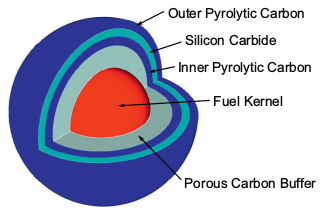
\includegraphics[height=3.5cm]{figures/triso}
	\caption{Drawing of a TRISO fuel particle. Image reproduced from \cite{hales_multidimensional_2013}.}
	\label{fig:triso}
\end{figure}

% Safety characteristics of HTGRs: Graphite and negative temp coeff
Graphite is another contributor to the passive safety of the \gls{HTGR} design.
Combining ceramic fuel and a graphite core structure permits high operating temperatures \cite{ballinger_balance_2004}.
Graphite has a high heat capacity and maintains its strength at temperatures beyond 2760 $^{\circ}$C.
Additionally, HTGRs have a negative temperature coefficient of reactivity and a low core power density.
A low core power density enables passive heat transfer mechanisms to remove the decay heat following postulated accidents \cite{neylan_modular_1988}.
These passive heat transfer mechanisms rely primarily on the natural processes of conduction, thermal radiation, and convection.
As a result, temperature changes in the core occur slowly and without damage to the core structure during transients.

% Co-generation applications: Rankine vs Bryton
HTGRs higher operating temperatures are a desirable feature because they offer increased thermal conversion efficiencies.
The early \gls{HTGR} designs converted their heat into electricity using the steam-Rankine cycle \cite{herranz_power_2009}.
In such a system, the helium coolant passes through a steam generator, and the steam drives a turbine.
This arrangement is around 38\% efficient \cite{breeze_nuclear_2014}.
However, the steam cycle requires a steam generator and also a gas circulator \cite{no_review_2007}.
This requirement increases the capital cost of power plant, and it creates a risk of a water ingress event.
The Brayton cycle is a better option because the helium coolant can directly drive a gas turbine in a closed cycle.
A closed cycle eliminates the need for a steam generator and a gas circulator.
Additionally, it removes external sources of contamination of the nuclear circuit, reducing the need for on-line cleanup systems \cite{iaea_current_2001}.
With the Brayton cycle, the system can achieve an energy conversion efficiency of around 48\% \cite{breeze_nuclear_2014}.

Higher outlet temperatures and increased thermal conversion efficiencies in HTGRs enable a wide range of process heat applications, such as coal gasification processes, oil refinery processes, and production of synthesis gas, methanol, and hydrogen.
Hydrogen offers a solution to energy and climate challenges, decarbonizing the transport and power sectors \cite{nagashima_japans_2018}.
Several hydrogen production processes benefit from high temperatures, such as high-temperature electrolysis \cite{doenitz_hydrogen_1980} or thermochemical water-splitting \cite{yildiz_efficiency_2006}.
Utilizing the \gls{HTGR} as the process energy source eliminates the need to burn fossil fuels to generate the steam those processes require \cite{iaea_current_2001}.

% Maybe this paragraph should be in objectives
This thesis focuses primarily on the \gls{MHTGR}-350 \cite{neylan_modular_1988} \cite{silady_licensing_1988}.
Under the sponsorship of the \gls{US} \gls{DOE}, a team consisting of General Atomics, Combustion Engineering, General Electric, Bechtel National, Stone \& Webster Engineering, and \gls{ORNL} developed the \gls{MHTGR}-350 \cite{neylan_modular_1988}.
They designed the basic module to deliver superheated steam at 17.3 MPa and 538 $^{\circ}$C.
Based on both economic and technological considerations, a 350 MWth modular reactor defines the optimal configuration.
The team completed in 1986 the preliminary safety information document for the MHTGR-350 and the complete draft pre-application in 1989 \cite{huning_steady_2014}.

% \cite{ballinger_balance_2004}
% The modular type HTGR provides the extra unique characteristic that the fuel temperature will not exceed the failure temperature following postulated accidents just by using passive heat transfer mechanisms.

\section{Motivation}

This work's ultimate goal is to support the development of \gls{HTGR} technology.
More specifically, we focus on the development of computational methods for modeling \glspl{HTGR} with \textit{Moltres} \cite{lindsay_introduction_2018} as our primary analysis tool.

% Why do we focus on HTGRs?
The Generation IV Roadmap project identified reactor concepts that could meet the future's energy demands in an efficient, economical, and environmentally safe manner \cite{macdonald_ngnp_2003}.
One of these reactor concepts is the \gls{VHTR}.
A \gls{VHTR} is a type of HTGR whose core outlet temperatures are between 700 and 950 $^{\circ}$C \cite{gif_gif_2019}.
The \gls{DOE} selected this reactor concept for the \gls{NGNP} Project.
This project intended to demonstrate emissions-free nuclear-assisted electricity and hydrogen production by 2015.

Although the \gls{DOE} canceled the \gls{NGNP} Project, the large scale deployment of HTGRs may become a reality in the near term.
Some microreactor designs embody this type of reactor technology and may be operational before 2030.
Additionally, as Section \ref{sec:pmr} has already described, HTGR technology has several favorable characteristics.
To recapitulate the most relevant features, the \gls{HTGR} relies on passive heat transfer mechanisms, uses TRISO particles as its fuel which inhibits proliferation, achieves high temperatures, and benefits from increased cycle efficiencies.
Another beneficial characteristic is that high temperatures enable a wide range of process heat applications, among which we find hydrogen production.

%Why is computational modeling important?
Modeling and prediction of core thermal-hydraulic behavior is necessary for assessing the safety characteristics of a reactor.
Determining the temperature inside a reactor, for both normal and transient operation, is of paramount importance as several materials' integrity depends on it.
Undesirably high temperatures endanger the TRISO particles' integrity and, consequently, jeopardize the fission product containment \cite{tak_numerical_2008}.
% The temperatures in the core have to be kept below values that begin to cause damage to fission product barriers, produce stmctural material weakness, and lead to excessive chemical reaction rates.
Furthermore, the complex fuel blocks geometry requires numerical calculations for obtaining the fuel temperatures.

The characteristics of an \gls{HTGR} are different from those of conventional \glspl{LWR}.
Such differences demand reactor analysis tools that capture the following peculiarities of \glspl{HTGR} \cite{rohde_development_2012}\cite{bostelmann_criticality_2016}:
\begin{itemize}
% \item Hexagonal structure: the shape of the fuel blocks hinders conformity to any orthogonal coordinate system.
\item Double heterogeneity: the TRISO particles form the first heterogeneity level, consisting of four
layers.
The second level arises from the fuel elements, as they encompass the compacts, the coolant, and the moderator.
\item Strong temperature dependence: the fuel temperatures have a significant effect on the neutron spectrum and the transient feedbacks.
\item High temperature gradient: the temperature difference between the fuel and the moderator is large during the course of transients.
\item High thermal inertia: the large graphite structures cause long transients.
\end{itemize}

%Why use Moltres?
Historically, linking a stand-alone neutronics solver to a thermal-hydraulics solver allowed for simulating an entire reactor.
The connection of the programs occurred in a loose-coupling fashion, such that one code's output served as the other's input and vice versa.
This coupling technique is commonly known as the operator-splitting technique \cite{ragusa_consistent_2009}.
In such an approach, each program uses a physical model that solves some of the problem variables while assuming constant the rest of them.
Nonetheless, these physical models describe processes that rely heavily on the solution of one another's.
The neutron flux determines the power distribution, and the power distribution strongly influences the temperature field.
Due to the \gls{HTGR} temperature feedback, the temperature affects the neutron flux distribution in the core.
Because of a strong temperature feedback, multiphysics transient simulations coupled via the operator-splitting approach may introduce significant numerical errors \cite{park_tightly_2010}\cite{ragusa_consistent_2009}.

\gls{MOOSE} \cite{gaston_moose_2009} is a computational framework targeted at solving fully coupled systems.
All the software built on the \gls{MOOSE} framework shares a joint code base.
These features facilitate relatively easy coupling between separate phenomena and allow for great flexibility, even with a large variance in time scales \cite{novak_pronghorn_2018}.
Additionally, all programs use \gls{MPI} for parallel communication and allow for deployment on massively-parallel cluster-computing platforms.

\textit{Moltres} is an open source, \gls{FEM} application built within the \gls{MOOSE} framework.
\textit{Moltres} solves arbitrary-group neutron diffusion, delayed neutron precursor concentration, and temperature governing equations.
All these characteristics, plus some modifications that this work intends to implement, make \textit{Moltres} suitable for solving the type of physical phenomena described above.

\section{Objectives}

% This thesis focuses on steady-state calculations and also intends to set a roadmap for the transient simulations.
As mentioned earlier, the ultimate goal of this work is to support the development of \gls{HTGR} technology.
The following list of main objectives expands on that goal.

\paragraph{Determine prismatic \glspl{HTGR} key physics.}
Prismatic HTGRs have inherent physics phenomena unique to their design.
This thesis intends to determine which are those inherent physics crucial for their accurate modeling.

\paragraph{Extend Moltres modeling capabilities to prismatic \glspl{HTGR}.}
Moltres is a multi-physics solver designed to capture key physics in \glspl{MSR}.
Moltres's current capabilities allow for solving some of the physics in the prismatic HTGR design.
Nevertheless, the solver needs to capture the missing physics in prismatic HTGRs and adequately integrate them into the current capabilities.

\paragraph{Understand \gls{HTGR} contribution to stopping climate change.}
HTGRs are an attractive technology due to attaining high temperatures.
With such high temperatures, the efficiency of hydrogen production increases.

\vskip 0.6cm
The main objectives are somewhat broad.
The following list presents secondary objectives which will lead to the fulfillment of the main objectives:

\paragraph{Demonstrate Moltres' ability to predict HTGR neutronics.}
A neutronics solver should predict the flux shape and magnitude accurately, during steady-state and transient simulations.
Previous work demonstrated Moltres' ability to solve MSR neutronics.
Chapter \ref{ch:neutronics} demonstrates such an ability for prismatic HTGRs.

\paragraph{Understand the impact of the group constants energy group structure on the HTGR diffusion calculations.}
The underlying physics of \glspl{HTGR} differ from the physics of other reactors.
Consequently, the simulation results will be sensitive to different parameters from other reactor type simulations.
Chapter \ref{ch:neutronics} studies the impact of the group constants energy group structure on the diffusion calculations.

\paragraph{Calculate power distribution correctly.}
The power distribution is the most influential parameter over the thermal-hydraulics as it determines the temperature profile in the reactor.
Previous work demonstrated Moltres ability to calculate the power distribution in MSRs.
Chapter \ref{ch:neutronics} evinces such an ability for prismatic HTGRs.

\paragraph{Predict prismatic HTGRs temperature profile accurately.}
Undesirably high temperatures endanger the integrity of the reactor structures, and most importantly, the TRISO particles.
Additionally, the temperature influences the neutronics.
Hence, an accurate neutronics calculation will be inaccurate without a correct thermal-hydraulics calculation. 
Previous work demonstrated Moltres ability to predict the temperature profile in MSRs.
Chapter \ref{ch:thermalfluids} examines Moltres ability to accurately predict the temperature profile in prismatic HTGRs.

\paragraph{Coupled simulations
Accurately model the thermal feedback on the neutronics.
Chapter \ref{ch:thermalfluids}

\paragraph{Techno-economic analysis of hydrogen production with HTGRs.}
High temperatures enable high-efficiency hydrogen production methods.
Most of them have different energy requirements and production rates.
Chapter \ref{ch:hydro} analyses such quantities.

\chapter{Methods}
\section{Moltres}

\section{MOOSE}

\section{Gmsh}

\section{Serpent}

\section{Cyclus}

\section{D3ploy}


\chapter{Neutronics}
\label{ch:neutronics}

This chapter presents several studies that use Moltres as a stand-alone neutronics solver.
The objective of the chapter is to validate Moltres calculation scheme by comparing Moltres results to Serpent and the OECD/NEA MHTGR-350 Benchmark.
This chapter comprehends the following sections: Section \ref{sec:neut-prelim} describes some preliminary studies that help set up Serpent and Moltres simulations, Section \ref{sec:neut-serpent} presents several studies comparing Moltres and Serpent results, Section \ref{sec:ph1e1} discusses Moltres results of Phase I Exercise 1 of the Benchmark, and Section \ref{sec:neutr-conc} concludes the chapter with a summary of the chapter and its key points.

\section{Preliminary studies}
\label{sec:neut-prelim}

This section's purpose is to find the right set up of Serpent and Moltres input files.
Section \ref{sec:homo-hetero} focuses on the materials definition in Serpent input file for obtaining the group constants for Moltres.
Section \ref{sec:setup} analyzes different ways to set up Moltres input files.

\subsection{Homogeneous vs. heterogeneous isotope distribution}
\label{sec:homo-hetero}

This section determines the proper way to treat the fuel compact heterogeneities in Serpent.
This study modeled in Serpent two different material distributions in a fuel compact: a homogeneous distribution of the isotopes and a heterogeneous distribution that explicitly modeled the TRISO particles.
The study used a hexagonal unit cell model that included the fuel compact, a helium gap, and the surrounding graphite, exhibited in Figure \ref{fig:compact-model}.
Table \ref{tab:compact} specifies the model input parameters.
The material temperature was 1200K, a case that represents the \gls{HFP} core state.
The Serpent simulations included 5$\times 10^4$ neutrons per cycle, 500 active cycles, and 50 inactive cycles for the calculations.
The homogeneous distribution simulation took 1.73 minutes and the heterogeneous distribution simulation 2.21 minutes using 256 cores --- the heterogeneous calculation took 28$\%$ longer.

\begin{figure}[htbp!]
  \centering
    \subfloat[Homogeneous isotope distribution in the fuel compact.]{
        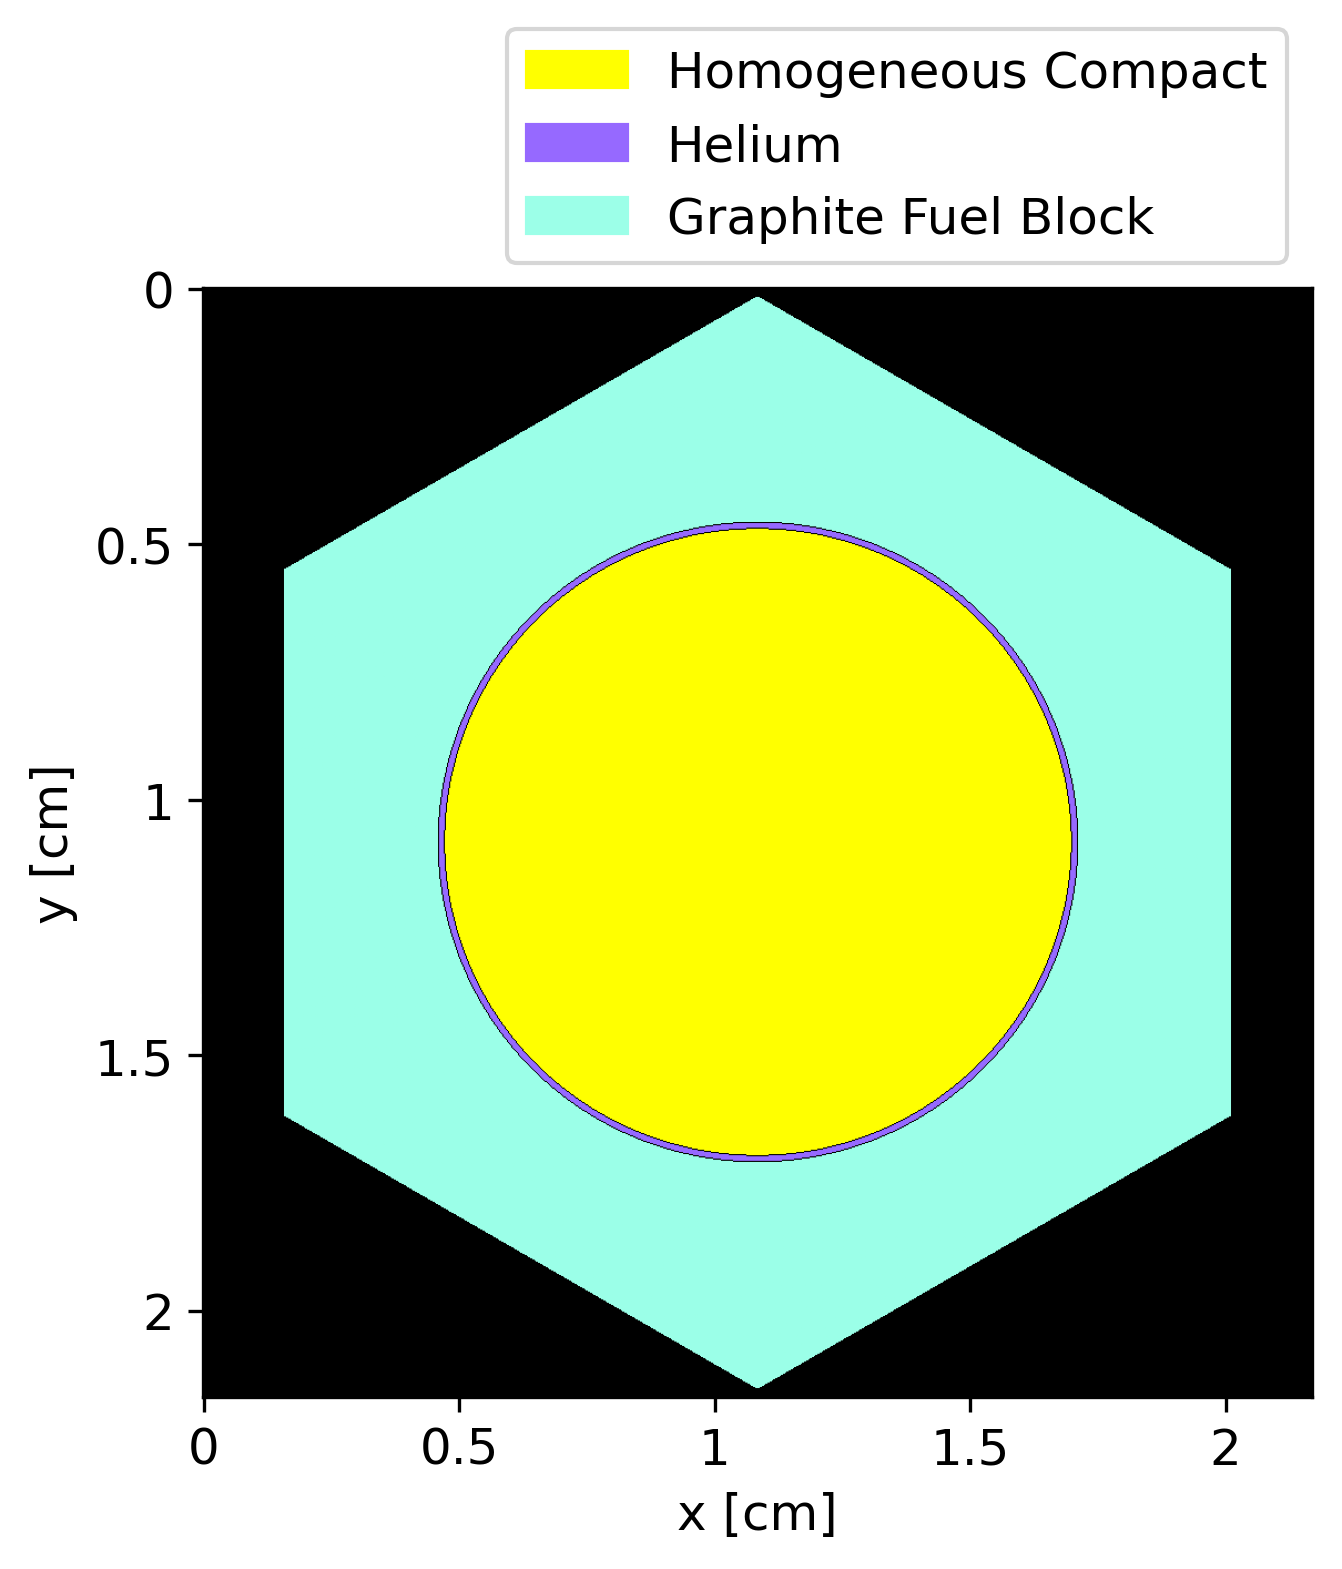
\includegraphics[width=0.45\textwidth]{figures-neutronics/compact-homo}
    }
    \subfloat[Explicit model of the TRISO particles in the fuel compact.]{
        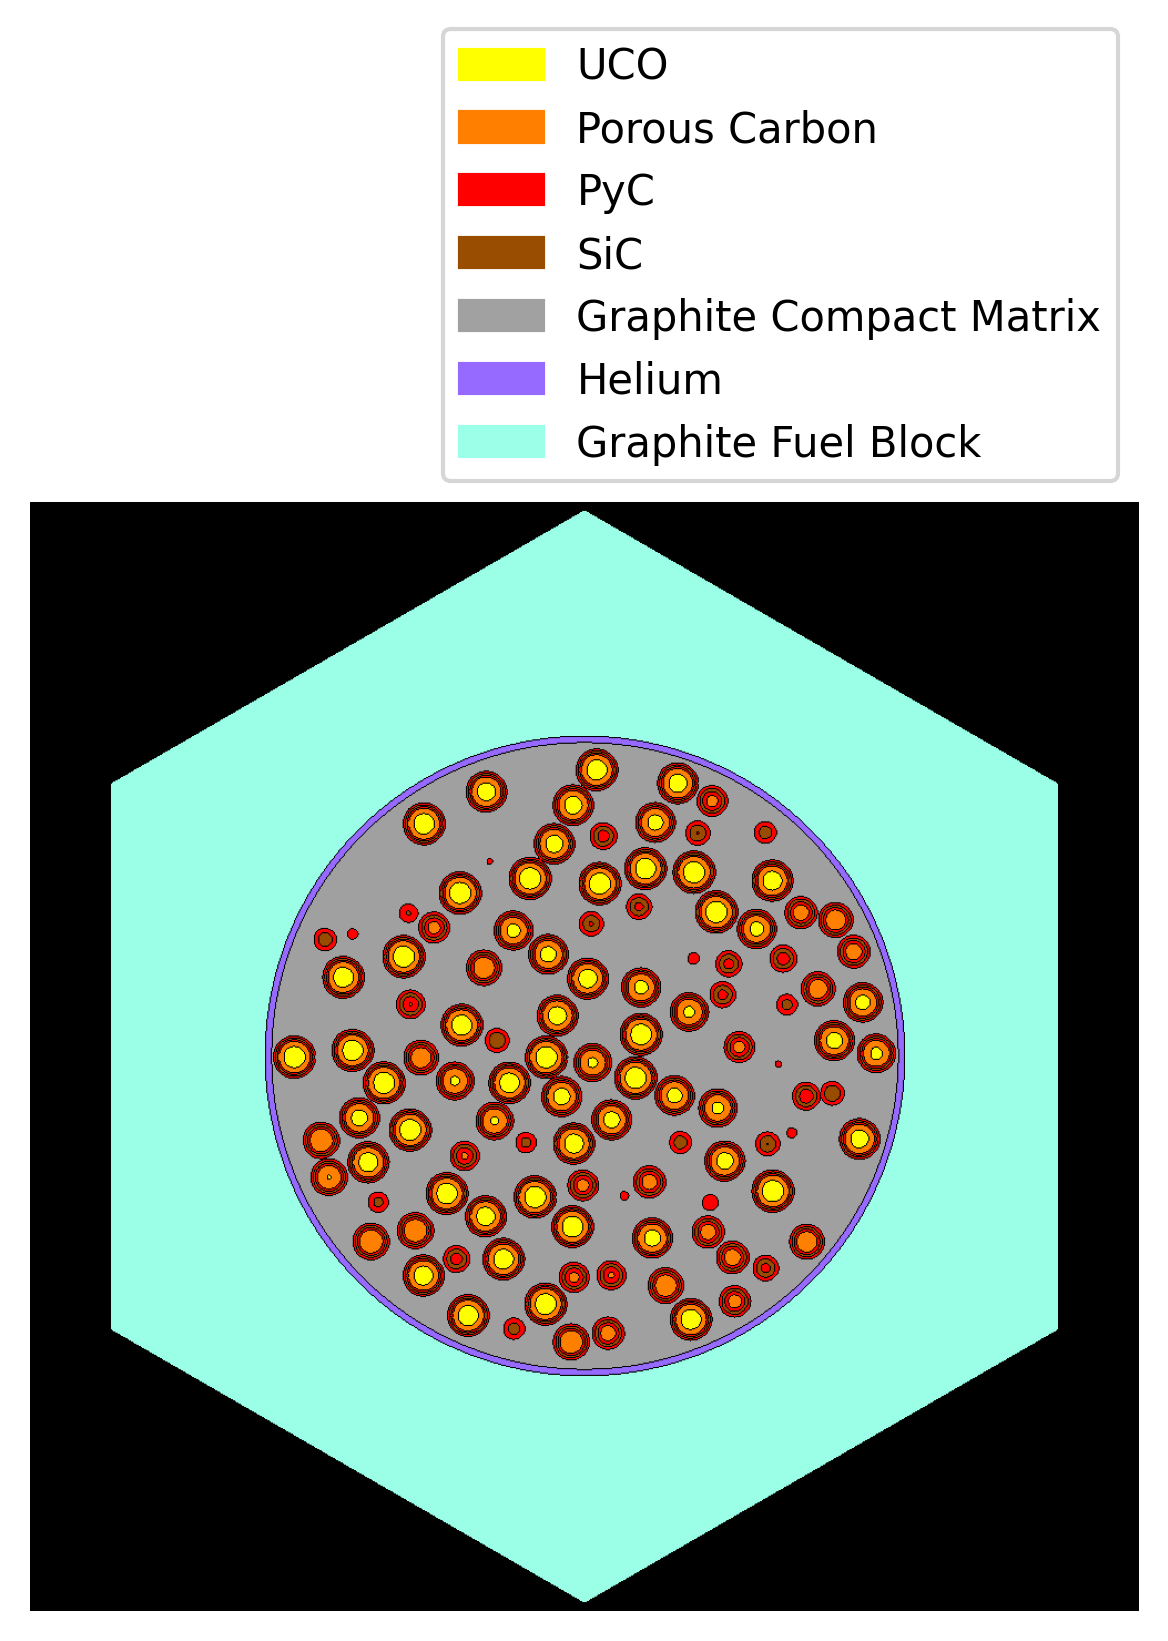
\includegraphics[width=0.45\textwidth]{figures-neutronics/compact}
    }
  \hfill
  \caption{Comparison of different Serpent models of the fuel compact.}
  \label{fig:compact-model}
\end{figure}

The \gls{Keff} was 1.17527 $\pm$ 0.00021 for the homogeneous distribution and 1.25107 $\pm$ 0.00020 for the heterogeneous distribution.
Serpent generated the group constants using the three energy group structure [0, 2.38eV, 111keV, 20MeV].
Using the heterogeneous distribution as the reference, a python script calculated the relative error of some of the group constants in an eigenvalue calculation.
The evaluated parameters were $D_g$, $\Sigma^r_g$, $\nu\Sigma^f_g$, and $\chi^t_g$ (see Equation \ref{eq:diffusion-eig}).
Figure \ref{fig:param-comparison} displays the relative errors for $\Sigma^r_g$ and $\nu\Sigma^f_g$, which were the group constants that changed the most.
The figure does not include $D_g$ and $\chi^t_g$ because their relative errors were less than 1$\%$.
The relative errors of $\Sigma^r_g$ and $\nu\Sigma^f_g$ were less than 6$\%$.

\begin{figure}[htbp!]
	\centering
	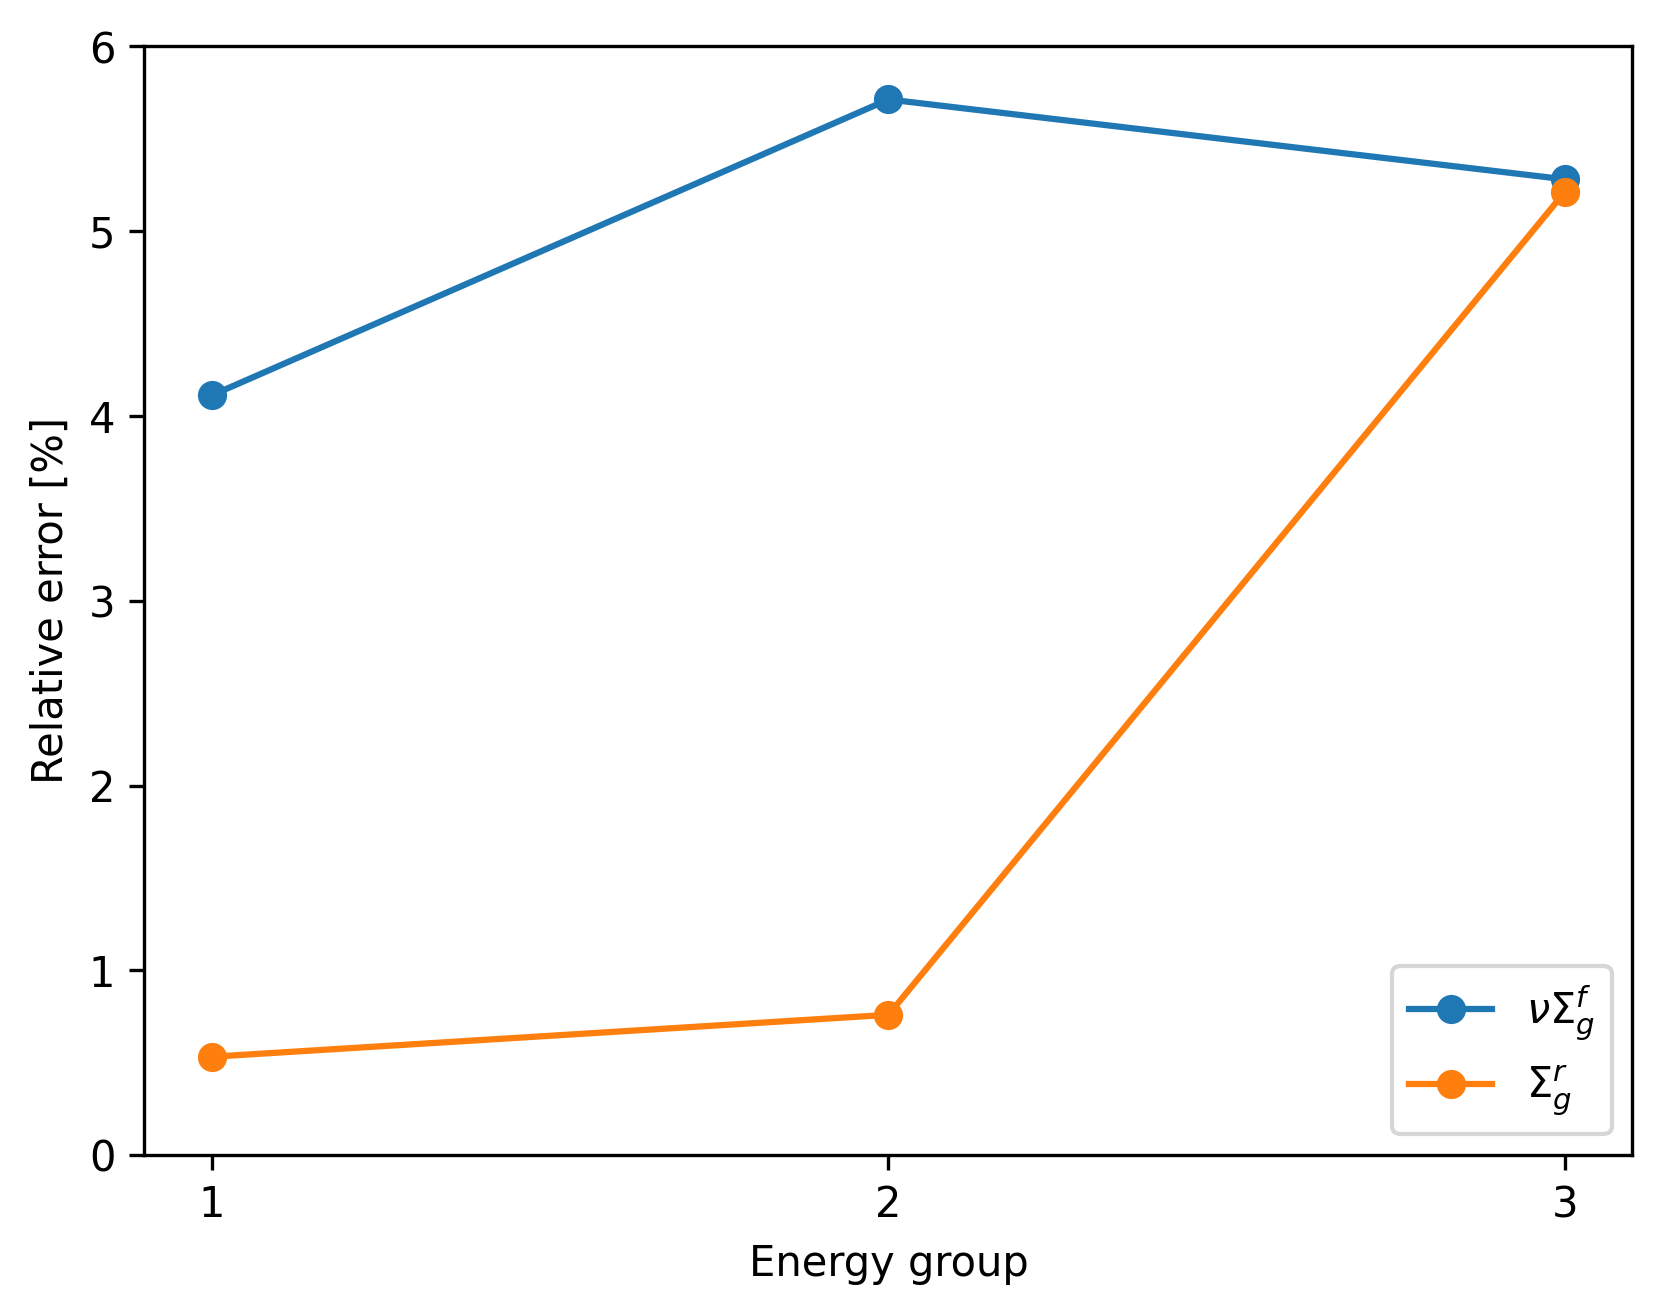
\includegraphics[width=0.43\linewidth]{figures-neutronics/param-comparison}
	\hfill
	\caption{Relative error of the group constants generated with a homogeneous isotope distribution vs explicit TRISO modeling.}
	\label{fig:param-comparison}
\end{figure}

The results show that the homogenization of the fuel compact isotopes decreases the multiplication factor considerably.
The impact on the group constants does not seem to be substantial; however, the multiplication factor's considerable difference suggests that the combined effect of the small variations in the group constants is significant.
Based on these results, Serpent models the TRISO particles explicitly for generating the group constants in the following sections.

\subsection{Problem set-up}
\label{sec:setup}

% Diffusion calculations: homo vs hetero in LWRs
Diffusion calculations necessitate a spatial homogenization of the group constants.
Depending on the desired level of detail, the type of homogenization could vary.
For example, in PWR core calculations, the homogenization in space could be per assembly or pin-by-pin \cite{krebs_calculational_1990}.
In a per-assembly homogenization, the diffusion solver represents the assembly as a single material neutronically (we will refer to diffusion calculations using this type as homogeneous calculations).
A pin-by-pin homogenization treats the pin or assembly heterogeneities, yielding a more detailed neutronic representation of the fuel assembly (we will refer to diffusion calculations of this type as heterogeneous calculations).

% Previous works using Moltres
Previous work \cite{lindsay_introduction_2018}\cite{pater_multiphysics_2019} used Moltres for simulating \glspl{MSR}, which allow for heterogeneous calculations.
In those calculations, the authors defined two materials in Moltres input files: the moderator and the fuel.
For such a configuration, a moderator mesh node holds the neutronics and temperature information only of the moderator.
The same is true in the fuel.
% On the other hand, a homogeneous calculation would not differentiate between moderator and fuel and would hold the information of both materials in each node.

% What I did in this section:
Keeping in mind Moltres proven capabilities, this work aimed for a heterogeneous calculation of a prismatic \gls{HTGR}.
For this study, Serpent modeled a fuel column of the MHTGR-350 and generated the group constants.
Figure \ref{fig:fuelcolumn} displays the Serpent model geometry.
Serpent generated the group constants for three materials: moderator, coolant, and fuel compact.
The Serpent simulations included 5$\times 10^5$ neutrons per cycle, 400 active cycles, and 100 inactive cycles for the calculations.
% The \gls{Keff} was 1.41933.
Taking advantage of the problem's symmetry, Moltres modeled only $1/12^{th}$ of the fuel column shown in Figure \ref{fig:fuelcolumn}.
I made the geometry and mesh using Gmsh \cite{geuzaine_gmsh_2020}.
The diffusion calculation had 1.84$\times 10^5$ \glspl{DoF} per energy-group.

\begin{figure}[htbp!]
	\centering
    \subfloat[Serpent model geometry.]{
        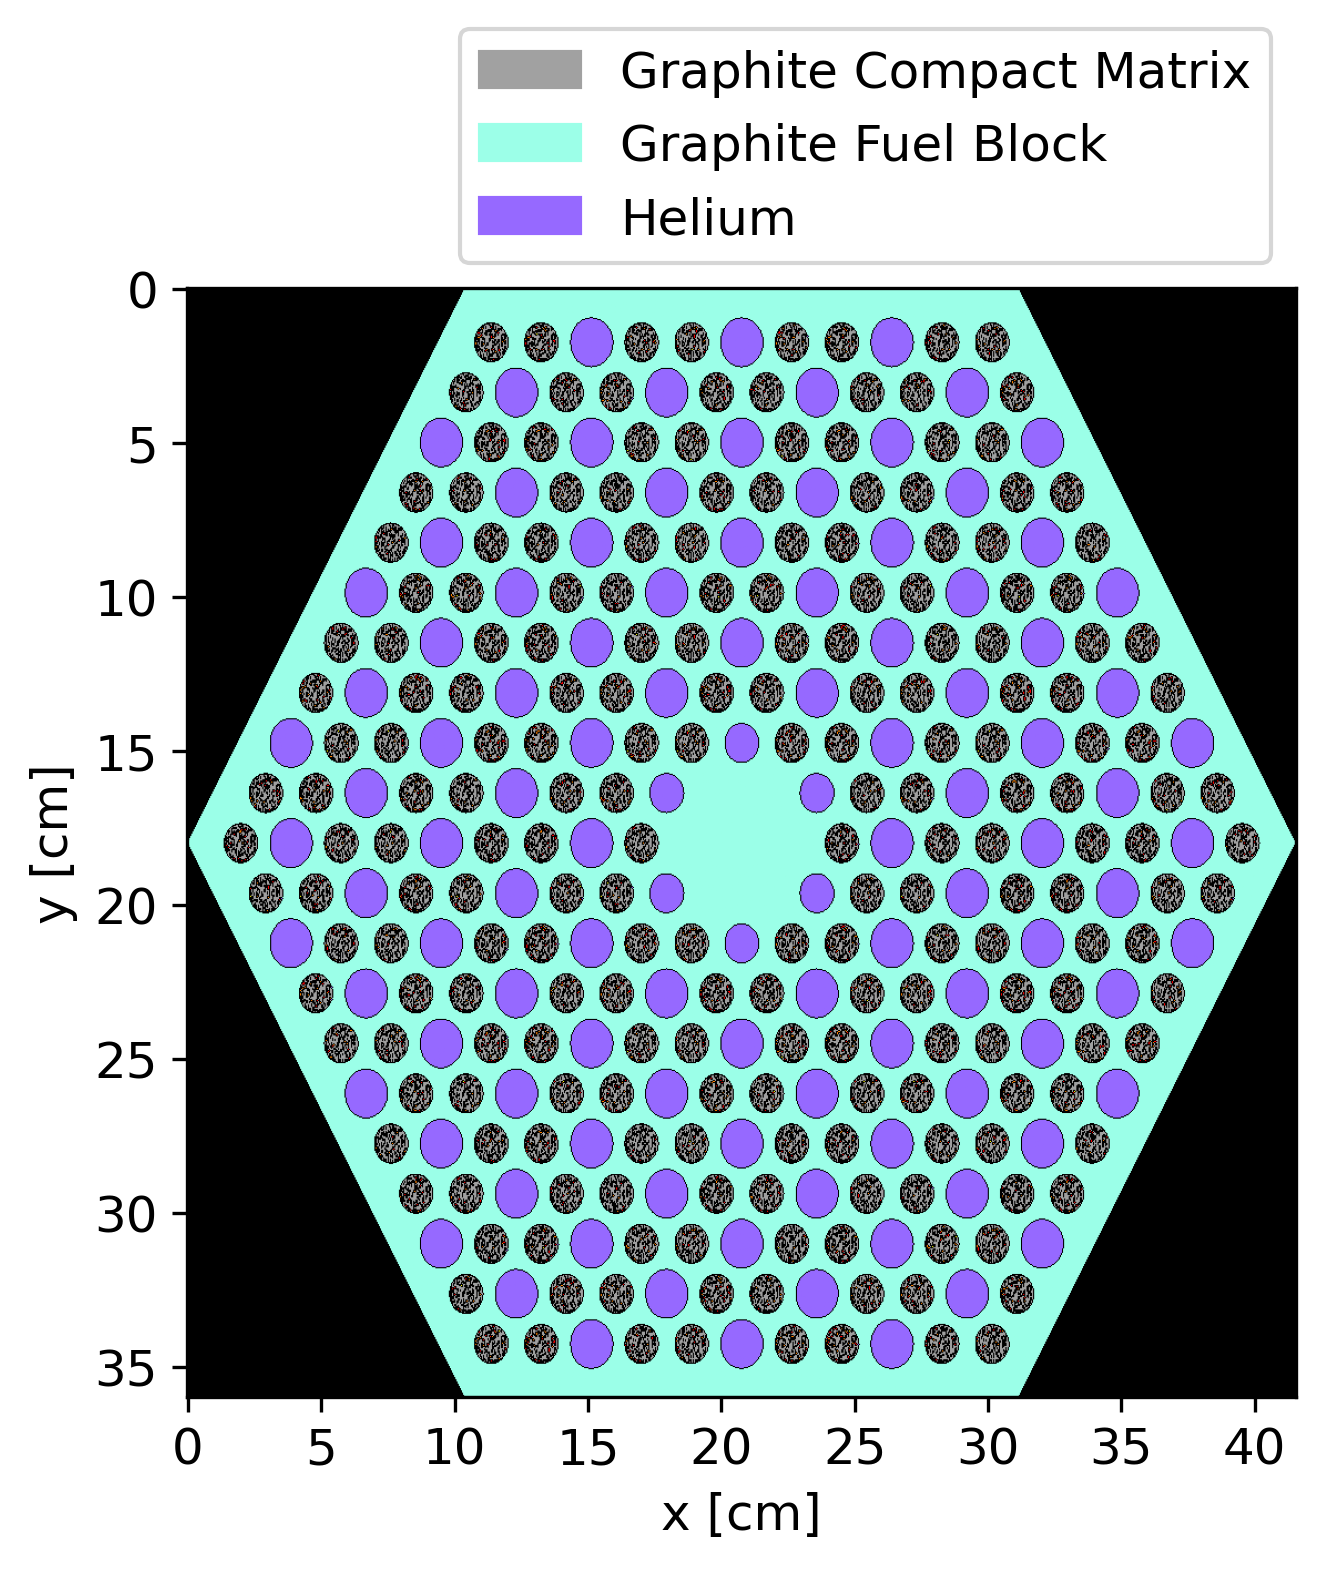
\includegraphics[width=0.35\textwidth]{figures-neutronics/standard}
    }
    \subfloat[Moltres model geometry.]{
        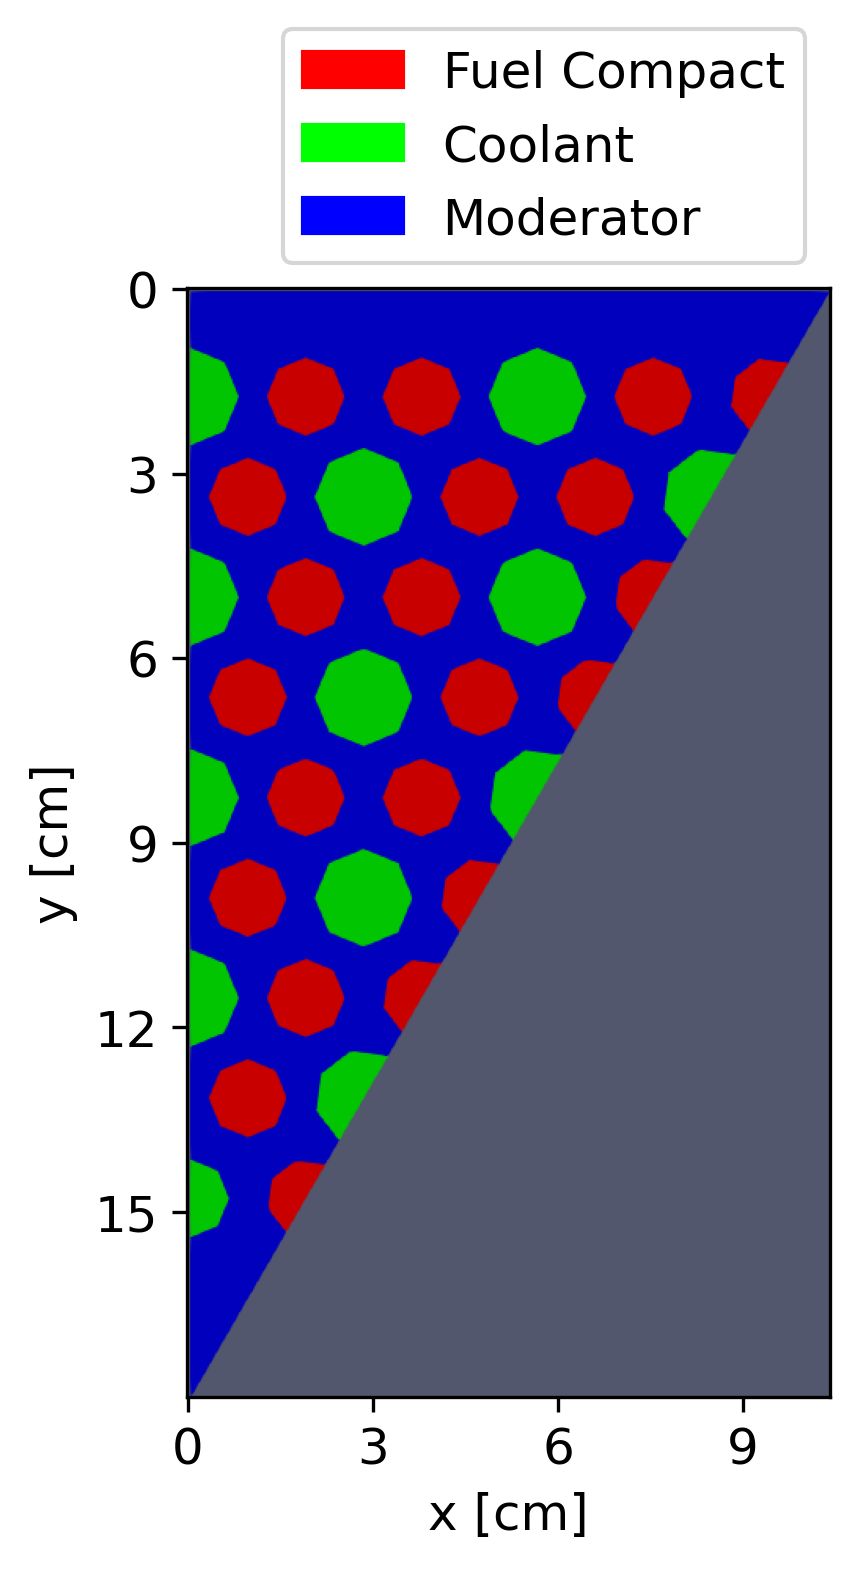
\includegraphics[width=0.22\textwidth]{figures-neutronics/3D-assembly-30deg-reflec-meshB2}
    }
	\hfill
    \caption{Fuel column of the MHTGR-350. $xy$-plane in the active core region.}
	\label{fig:fuelcolumn}
\end{figure}

Moltres simulation obeyed an eigenvalue convergence tolerance of 1$\times$10$^{-8}$, defined by equation \ref{eq:moltres-tol}

\begin{align}
   & \frac{k^{(n)}-k^{(n-1)}}{k^{(n)}} < \varepsilon \label{eq:moltres-tol}
   \intertext{where}
   & k^{(n)} = \mbox{eigenvalue at iteration $n$ } [-] \notag \\
   & \varepsilon = \mbox{convergence tolerance } [-]. \notag
\end{align}

The calculation used two energy groups with the structure [0, 0.625eV, 20MeV].
The eigenvalue calculation did not converge.
Although several factors could contribute to this behavior, I focused on the validity of the diffusion calculations in this system.

% Diffusion validity see bu1/tools-bu.txt
In diffusion theory, the current density $J$ is proportional to the gradient of the flux, see equation \ref{eq:diff} \cite{leppanen_development_2007}.
\begin{align}
   & J = - D \nabla \phi \label{eq:diff} \\
   \intertext{where}
   & J = \mbox{current density } [n \cdot cm^{-2} \cdot s^{-1}] \notag \\
   & D = \mbox{diffusion coefficient } [cm] \notag \\
   & \phi = \mbox{neutron flux } [n \cdot cm^{-2} \cdot s^{-1}]. \notag
\end{align}

This approximation relies on the following assumptions:
\begin{itemize}
	\item the angular flux does not depend strongly on the angular variables,
	\item the fission source is isotropic,
	\item the time derivative of the current density is small compared to the mean collision time,
	\item and the anisotropic energy-transfer due to scattering is negligible in group-to-group scattering.
\end{itemize}

More detailed studies of the transport equation indicate that the following cases violate the assumption of a weak angular dependence \cite{duderstadt_nuclear_1976}:
\begin{itemize}
    \item regions near vacuum boundaries and low-density material regions,
    \item regions near strongly absorbing media,
    \item and regions near localized sources.
\end{itemize}

The diffusion theory applies best to geometries consisting of large homogeneous regions where the flux gradient is small.
This is the case for material regions whose geometrical scales are considerably larger than the neutron mean free path.
For this reason, Table \ref{tab:mfp} compares the neutron mean free path in the different fuel assembly materials.
The mean free path in the fuel compact and the moderator are in the order of the centimeters.
In the coolant, the mean free path magnitude is comparable to the fuel column dimensions.
These results suggest that a heterogeneous diffusion calculation of the prismatic fuel column challenges some of the diffusion theory assumptions.

\begin{table}[htbp!]
  \centering
  \caption{Neutron mean free path in different materials. Values expressed in $cm$.}
  \begin{tabular}{l|cccc}
  \toprule
              & Fuel compact  & Moderator  & Coolant  & Homogeneous fuel \\
  \midrule
  Fast  		  & 2.71 & 2.70 & 1137.31 & 3.37 \\
  Thermal		  & 2.22 & 2.36 & 1945.49 & 2.89 \\
  \bottomrule
  \end{tabular}
  \label{tab:mfp}
\end{table}

Next, I conducted a feasibility study for the homogeneous calculation of the fuel assembly in Moltres.
Serpent calculated the homogeneous group constants of the fuel assembly, see equation \ref{eq:diffusion-eig}, by homogenizing the fuel, coolant, and moderator.
This material's mean free path is in the order of the centimeters, Table \ref{tab:mfp}.
Next, Moltres used the homogeneous group constants to carry out an eigenvalue calculation.
Comparing Moltres results with Serpent results, Serpent's \gls{Keff} was 1.41942 $\pm$ 0.00007 while Moltres' was 1.40788.
Moltres eigenvalue is smaller than Serpent's eigenvalue.
% This difference is possibly due to the lack of treatment of the anisotropic term in the scattering cross-section.
Additionally, Figure \ref{fig:prelim} displays a comparison between the axial flux in the fuel column obtained with Serpent vs. Moltres.
Serpent's flux is the average value of the flux in each bin, while Moltres flux is the point-wise flux over the $z$-axis
\begin{align}
  & \phi_s(z) = \frac{\int_{\Delta V} \phi(x,y,z) dV}{\Delta V} \label{eq:serpent-flux} \\
  & \phi_m(z) = \phi_m(x,y,z)   \label{eq:moltres-flux}
  \intertext{where}
  & \phi_s(z) = \mbox{Serpent axial flux } [n \cdot cm^{-2} \cdot s^{-1}] \notag \\
  & \Delta V = \mbox{Volume of the detector bins } [cm^3] \notag \\
  & \phi_m(z) = \mbox{Moltres axial flux } [n \cdot cm^{-2} \cdot s^{-1}]. \notag
\end{align}

The fluxes are similar in shape and magnitude.
% Conclusion
I emphasize that this was a feasibility study.
The following sections present a more in-depth analysis of more detailed results.
Based on these results and discussion, I conducted homogeneous calculations using Moltres in the following sections.

\begin{figure}[htbp!]
	\centering
    \subfloat[Serpent axial flux.]{
        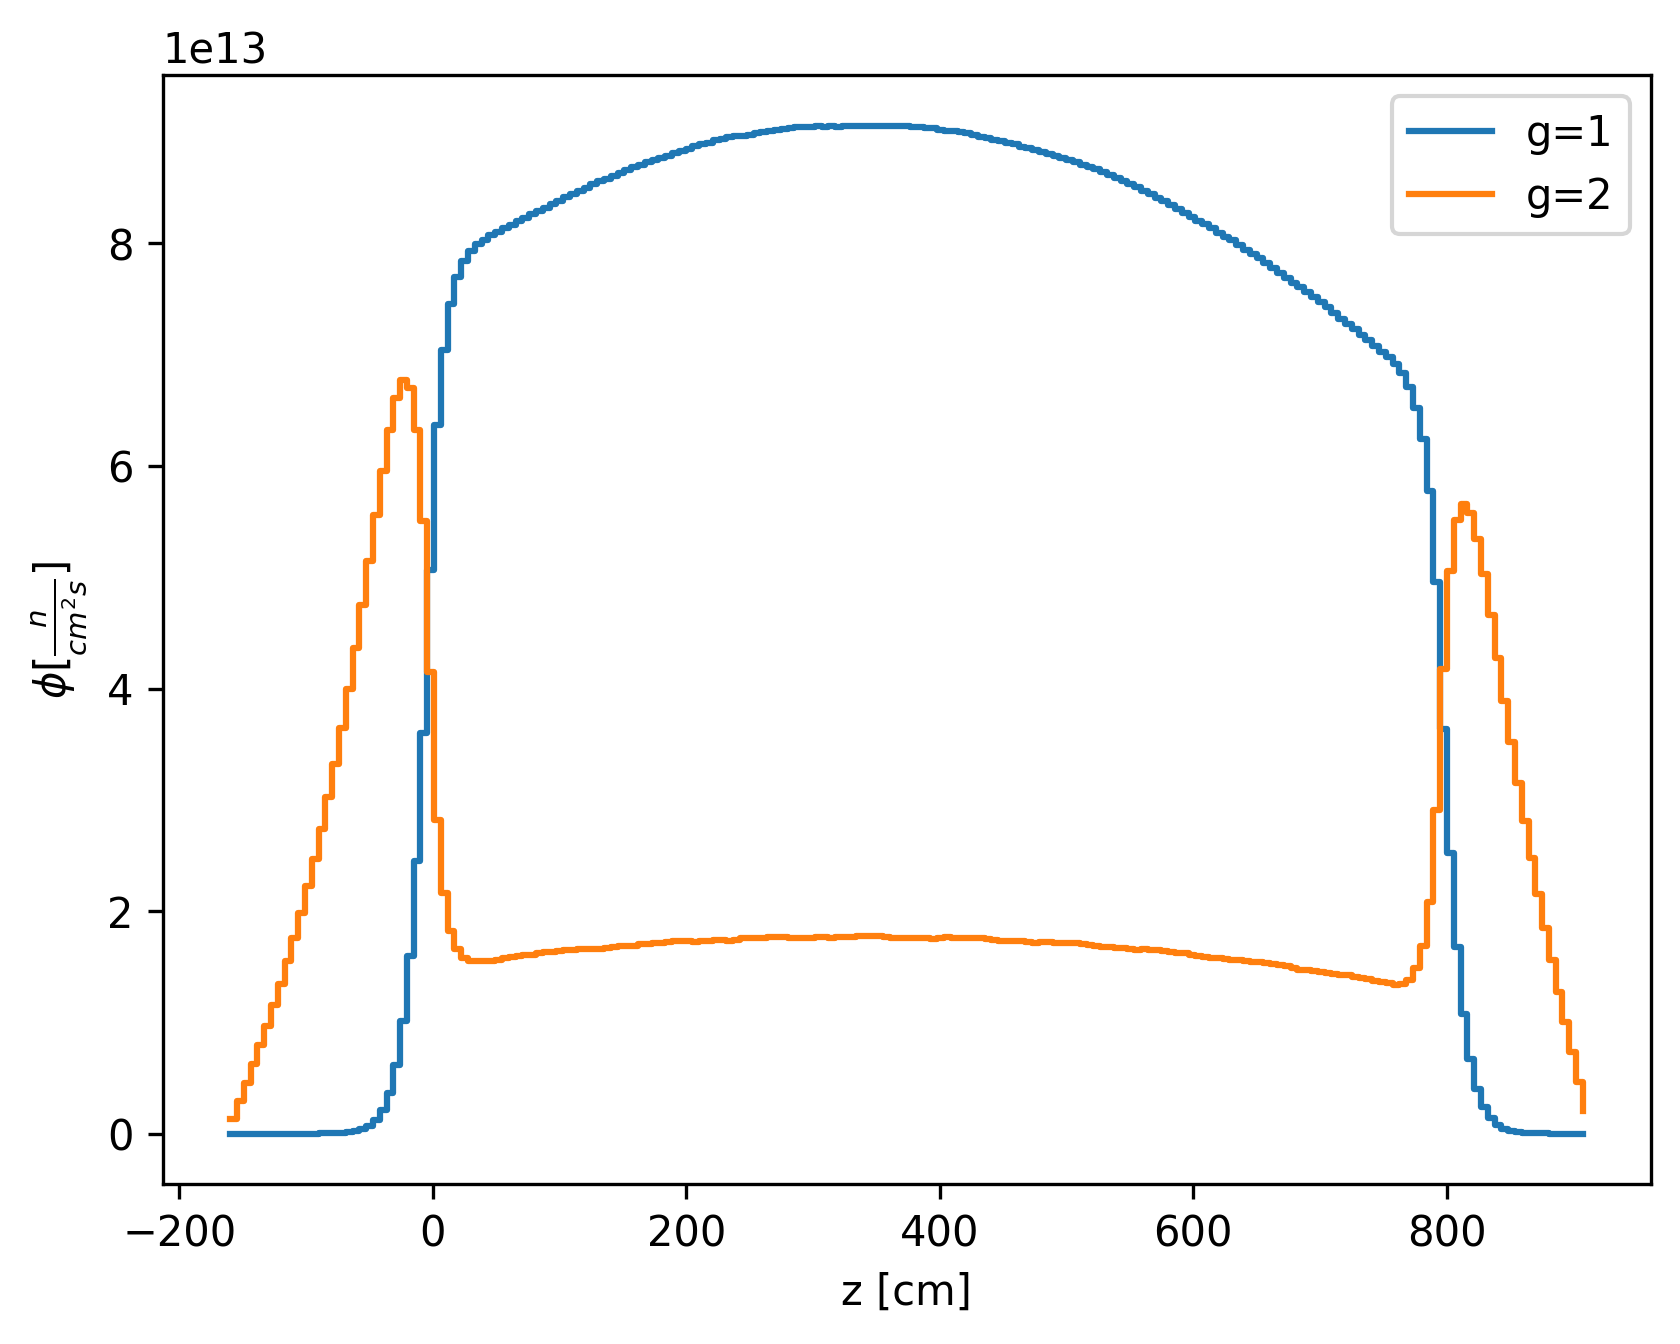
\includegraphics[width=0.45\textwidth]{figures-neutronics/standard-column-detector-Axial}
    }
    \subfloat[Moltres axial flux.]{
        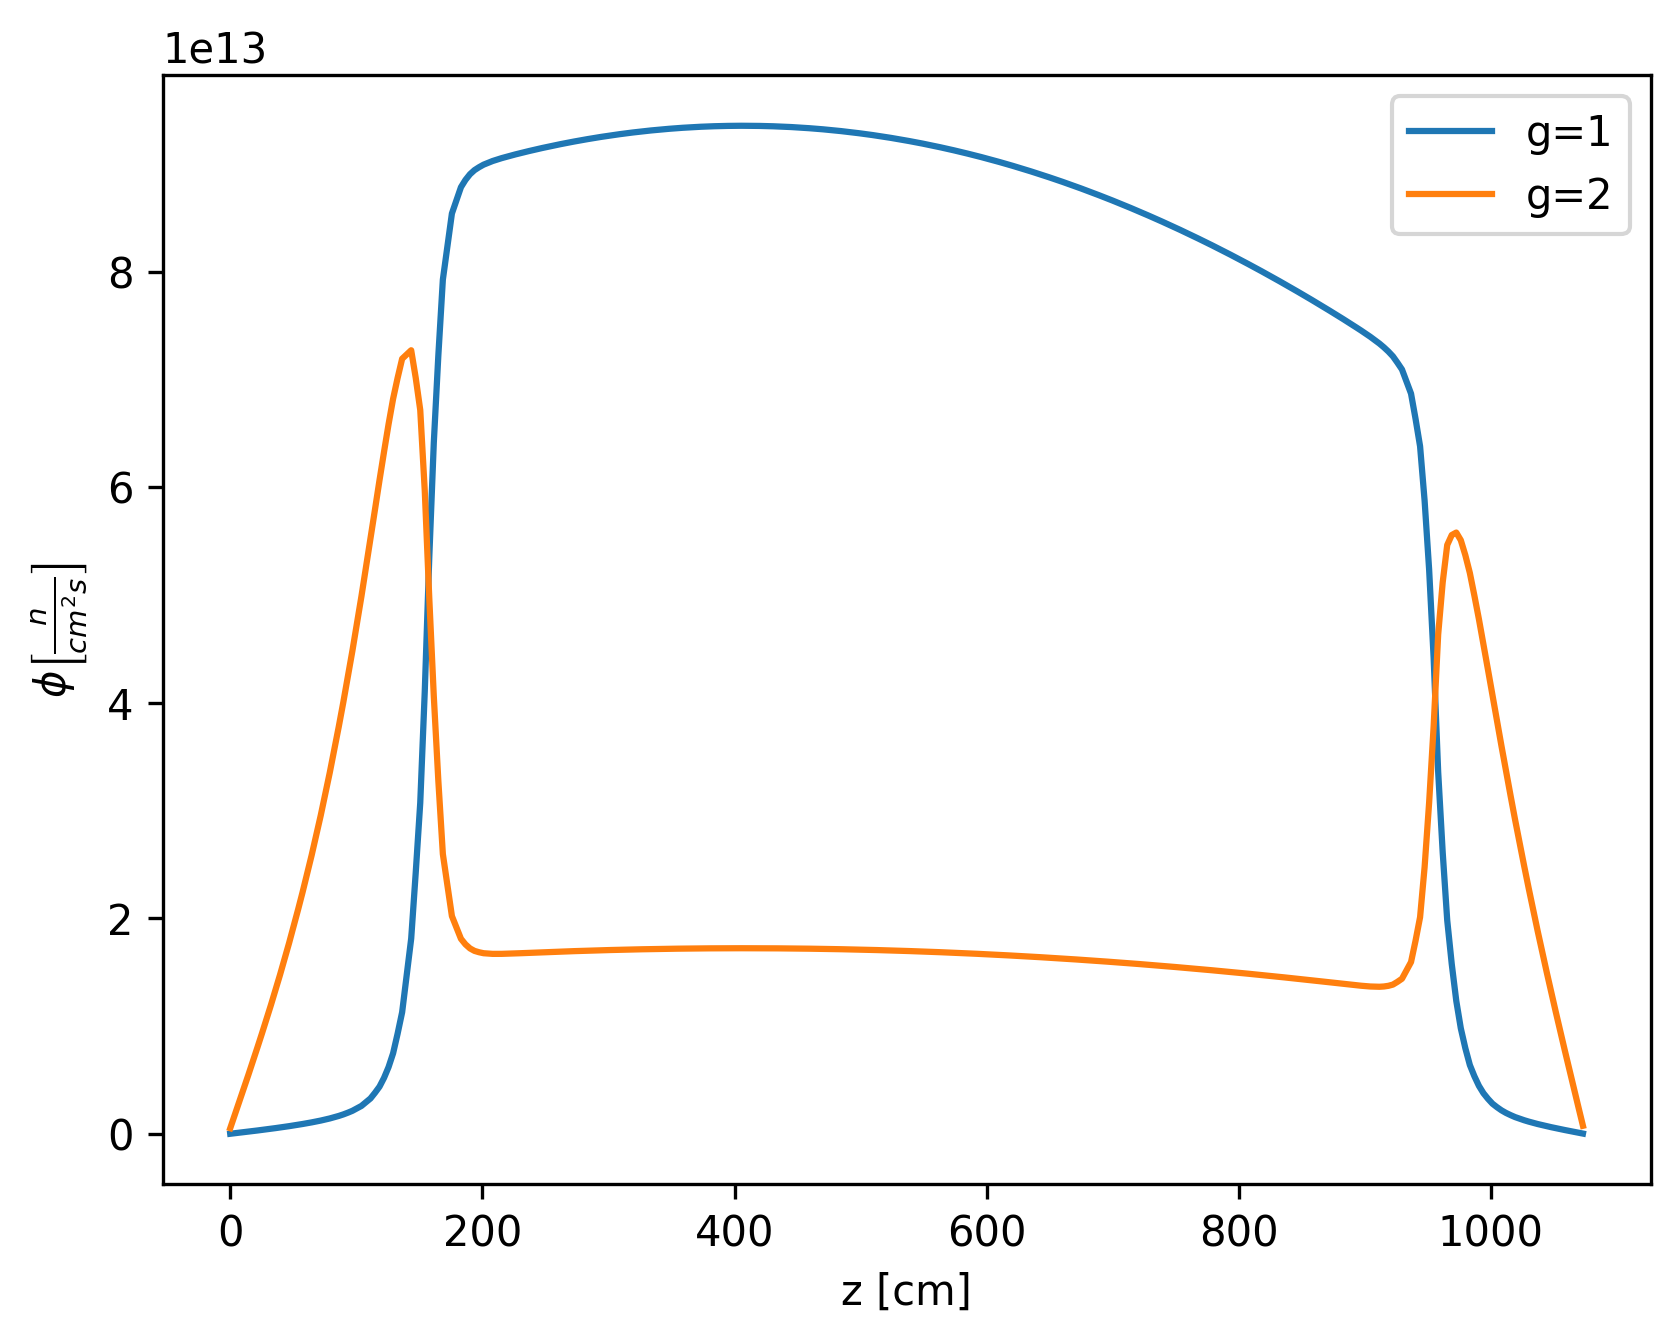
\includegraphics[width=0.45\textwidth]{figures-neutronics/homo-fuel}
    }
	\hfill
  \caption{Comparison of the two group axial flux in the fuel column.}
	\label{fig:prelim}
\end{figure}

\section{Serpent-Moltres comparison}
\label{sec:neut-serpent}

In this section, Serpent modeled a fuel column and the full-core of the MHTGR-350.
Serpent obtained the homogenized group constants that served as input to Moltres.
The following sections compare Moltres and Serpent results as a validation exercise.

\subsection{Fuel column}

This section investigats the effects of the energy group structure on the diffusion simulations.
I conducted two analyses: first, I varied the number of energy groups, second, I varied the energy group structures with a constant number of energy groups.
To reduce the computational expense, we narrowed down our focus to a fuel column of the MHTGR-350, Figure \ref{fig:fuelcolumn}.
% The fuel column includes the bottom and top reflectors.
Tables \ref{tab:element-characteristics} and \ref{tab:compact} specify the model input parameters.

The first step in the calculation was to obtain the group constants using Serpent.
Figure \ref{fig:fuelcolumn} displays the axial layout of the model.
Serpent's model did not consider the fuel handling holes or the bottom and top reflectors' coolant channels for simplicity.
\glspl{HTGR} use burnable poisons to reduce the power peaking factors in various active core regions.
Some reactors have burnable poisons in the rings closer to the reflectors, and no burnable poisons in the middle rings.
This characteristic motivated the analysis of two cases: one fuel column that does not have burnable poisons and one that does.
The burnable poisons' locations are the six corners of the fuel assembly, Figure \ref{fig:fuelassembly}.
The material temperatures were 600 and 1200K, cases that represent the \gls{CZP} and the \gls{HFP} core states.
The Serpent simulations included 4$\times 10^5$ neutrons/cycle, 360 active cycles, and 40 inactive cycles for the calculations.

Taking advantage of the problem's symmetry, Moltres modeled only $1/12^{th}$ of the homogenized fuel column.
I made the geometry and mesh, which had 3.71 $\times 10^4$ elements and 2.29 $\times 10^4$ nodes, using Gmsh.
The diffusion calculations had 2.29 $\times 10^4$ \glspl{DoF} per energy-group.
The Moltres input files set an eigenvalue and a flux convergence tolerance of 1$\times$10$^{-8}$.
Moltres calculations used the different energy group structures listed in Table \ref{tab:energygroups}.

\begin{table}[htbp!]
  \centering
  \caption{Energy group structure \cite{iaea_evaluation_2003}.}
  \begin{tabular}{S[table-format=2.2e-1]|llllllllllll}
  \toprule
                      & \multicolumn{12}{c}{Group structure} \\
  \multicolumn{1}{c|}{Upper boundary [eV]} & 26    & 21   & 18   & 15a & 15b & 15c & 15d & 15e   & 12  & 9  & 6  & 3 \\
  \midrule
  1.49e+07            & 1     & 1    & 1    & 1   & 1   & 1   & 1   & 1     & 1   & 1  & 1  & 1 \\ 
  7.41e+06            & 2     &      &      &     &     &     &     &       &     &    &    &   \\ 
  3.68e+06            & 3     & 2    & 2    & 2   & 2   & 2   & 2   & 2     & 2   &    &    &   \\ 
  6.72e+05            & 4     &      &      &     &     &     &     &       &     &    &    &   \\ 
  1.11e+05            & 5     & 3    & 3    & 3   & 3   & 3   & 3   & 3     & 3   & 2  & 2  & 2 \\ 
  1.93e+04            & 6     & 4    & 4    & 4   & 4   &     &     &       & 4   &    &    &   \\ 
  3.35e+03            & 7     &      &      &     &     &     &     &       &     &    &    &   \\ 
  1.58e+03            & 8     & 5    & 5    &     &     & 4   &     &       &     &    &    &   \\ 
  7.48e+02            & 9     & 6    & 6    & 5   & 5   &     & 4   & 4     & 5   & 3  &    &   \\ 
  2.75e+02            & 10    & 7    & 7    & 6   & 6   & 5   &     &       & 6   & 4  &    &   \\ 
  1.30e+02            & 11    & 8    & 8    & 7   & 7   &     & 5   & 5     & 7   & 5  & 3  &   \\ 
  6.14e+01            & 12    & 9    &      &     & 8   & 6   &     &       &     &    &    &   \\ 
  2.90e+01            & 13    & 10   & 9    & 8   & 9   &     & 6   & 6     &     &    &    &   \\ 
  1.37e+01            & 14    & 11   & 10   & 9   &     &     &     &       & 8   & 6  &    &   \\ 
  8.32e+00            & 15    & 12   & 11   & 10  & 10  & 7   & 7   & 7     & 9   &    &    &   \\ 
  5.04e+00            & 16    &      &      &     &     &     &     &       &     &    &    &   \\ 
  2.38e+00            & 17    & 13   & 12   & 11  & 11  & 8   & 8   & 8     & 10  & 7  & 4  & 3 \\ 
  1.29e+00            & 18    & 14   &      &     &     &     &     &       &     &    &    &   \\ 
  6.50e-01            & 19    & 15   & 13   & 12  & 12  & 9   & 9   & 9     & 11  & 8  & 5  &   \\ 
  3.50e-01            & 20    & 16   &      &     &     & 10  & 10  &       &     &    &    &   \\ 
  2.00e-01            & 21    & 17   & 14   & 13  & 13  & 11  & 11  & 10    &     &    &    &   \\ 
  1.20e-01            & 22    &      &      &     &     &     &     & 11    &     &    &    &   \\ 
  8.00e-02            & 23    & 18   & 15   & 14  & 14  & 12  & 12  & 12    &     &    &    &   \\ 
  5.00e-02            & 24    & 19   & 16   &     &     & 13  & 13  & 13    &     &    &    &   \\ 
  2.00e-02            & 25    & 20   & 17   & 15  & 15  & 14  & 14  & 14    & 12  & 9  & 6  &   \\ 
  1.00e-02            & 26    & 21   & 18   &     &     & 15  & 15  & 15    &     &    &    &   \\ 
  \bottomrule
  \end{tabular}
  \label{tab:energygroups}
\end{table}

% Fluxes
To recapitulate, we simulated four operational cases: 
\begin{itemize}
  \item Operational case 1: fuel with no burnable poisons at 600K.
  \item Operational case 2: fuel with no burnable poisons at 1200K.
  \item Operational case 3: fuel with burnable poisons at 600K.
  \item Operational case 4: fuel with burnable poisons at 1200K.
\end{itemize}

% This is very important and I should review it carefully
To compare the results from Serpent and Moltres, we review the three-group axial fluxes found by each of them.
Moltres ran the calculations for 26 energy groups and collapsed the results into three energy groups to facilitate the results' visualization.
Figures \ref{fig:assembly-noLBP-600-flux} to \ref{fig:assembly-LBP-1200-flux} display the axial flux from the Serpent and the Moltres simulations for all cases.
For the operational case 1, the fluxes are close in shape and magnitude.
For the operational case 2, the fluxes look similar.
The flux in Moltres has a straighter shape.
The thermal flux peak in the bottom reflector is bigger.
For the operational case 3, the flux in Moltres has a larger magnitude.
Additionally, the shape of the Moltres flux is concave, while the Serpent flux is convex.
For the operational case 4, the flux in Moltres is larger and more concave than Serpent flux.
Overall, the fluxes in Moltres and Serpent are close in shape and magnitude.

% No LBP 600
\begin{figure}[htbp!]
	\centering
    \subfloat[Serpent neutron flux.]{
        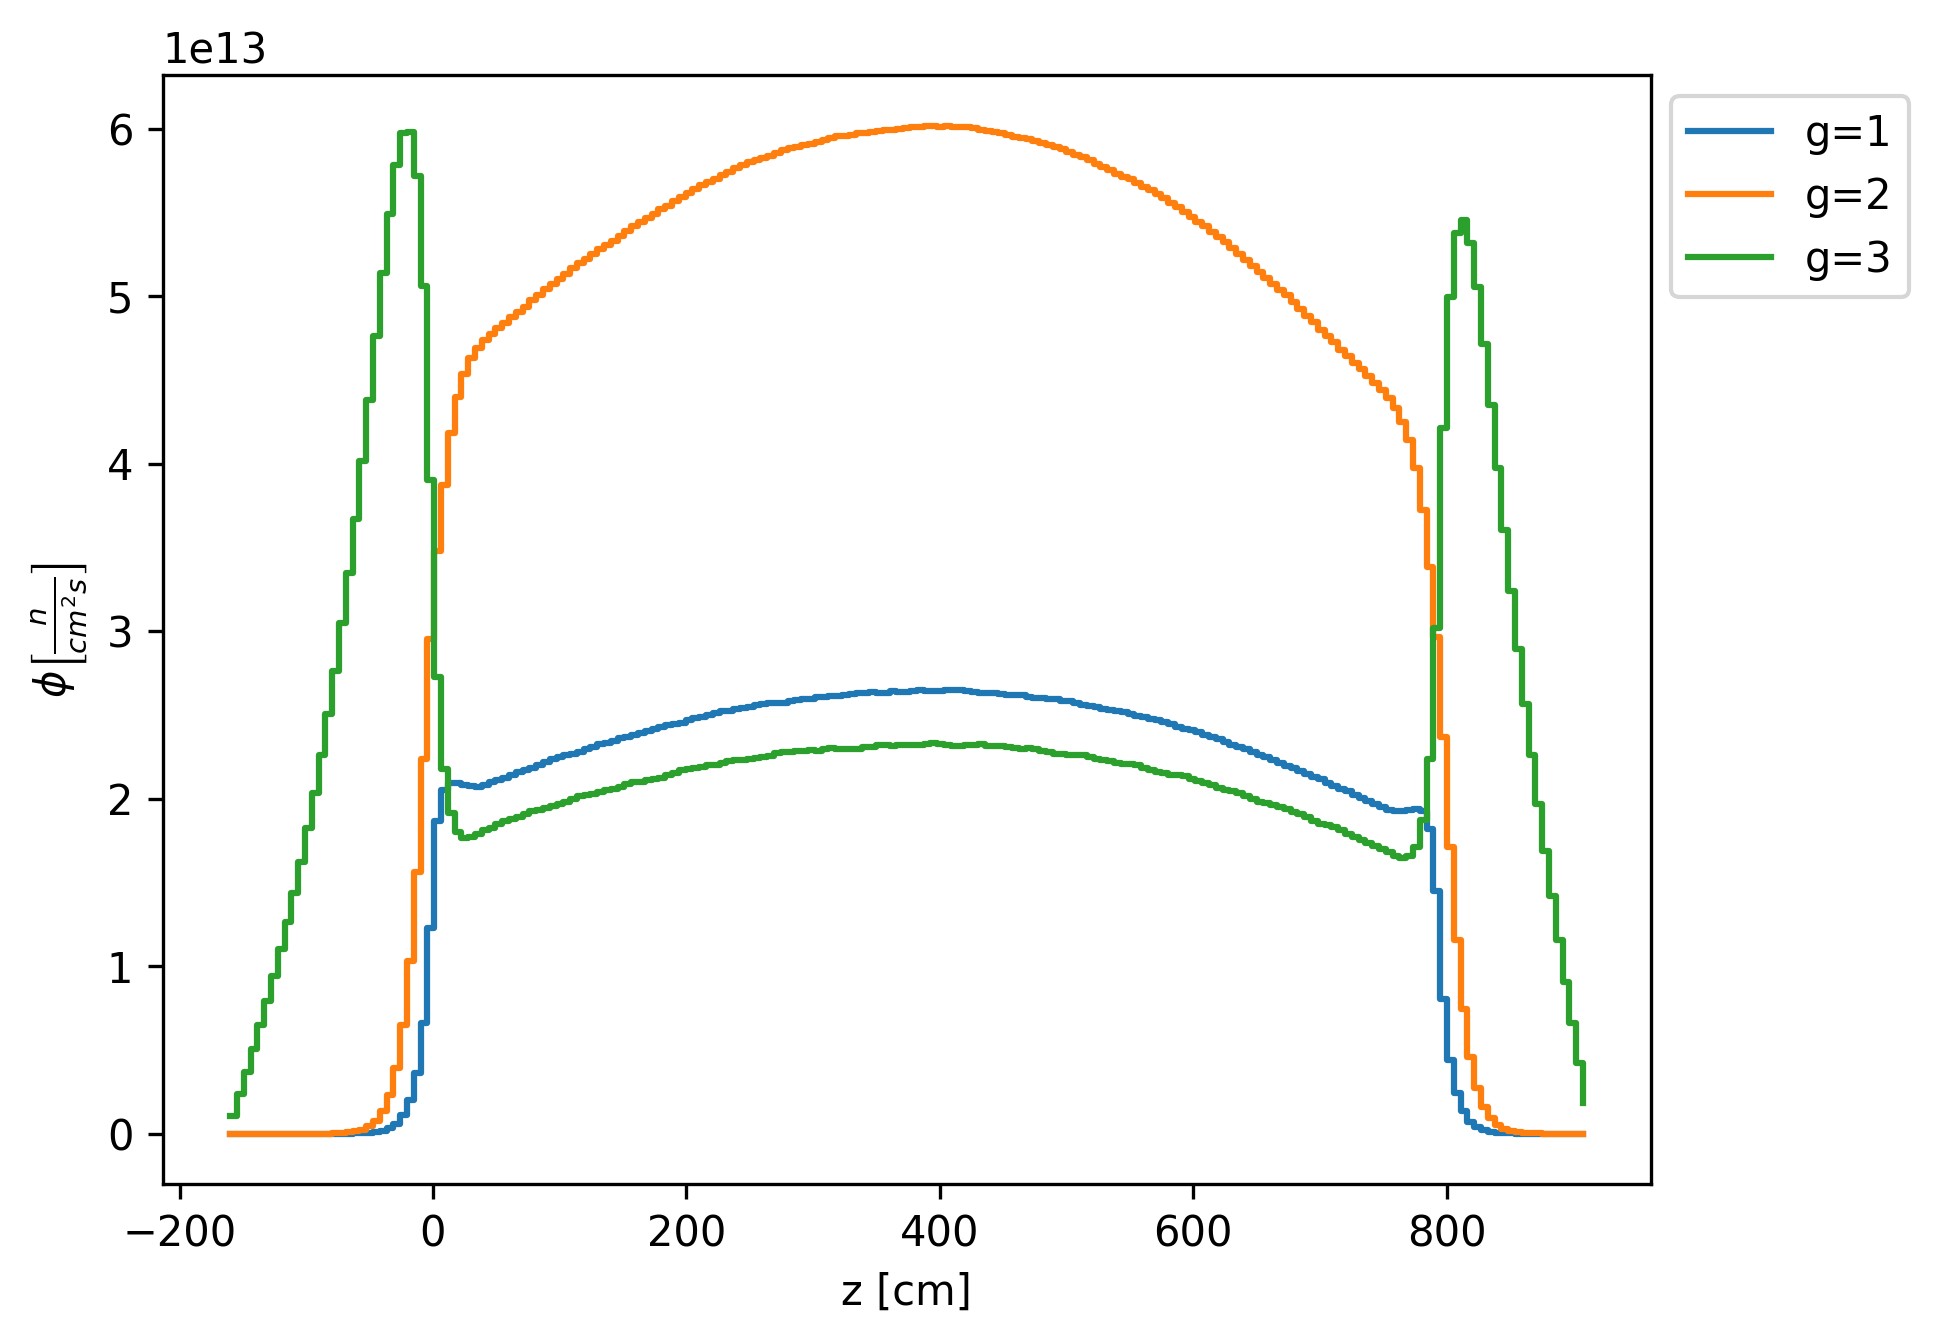
\includegraphics[width=0.45\textwidth]{figures-neutronics/serpent26G-noLBP-600-collapse}
    }
    \subfloat[Moltres neutron flux.]{
        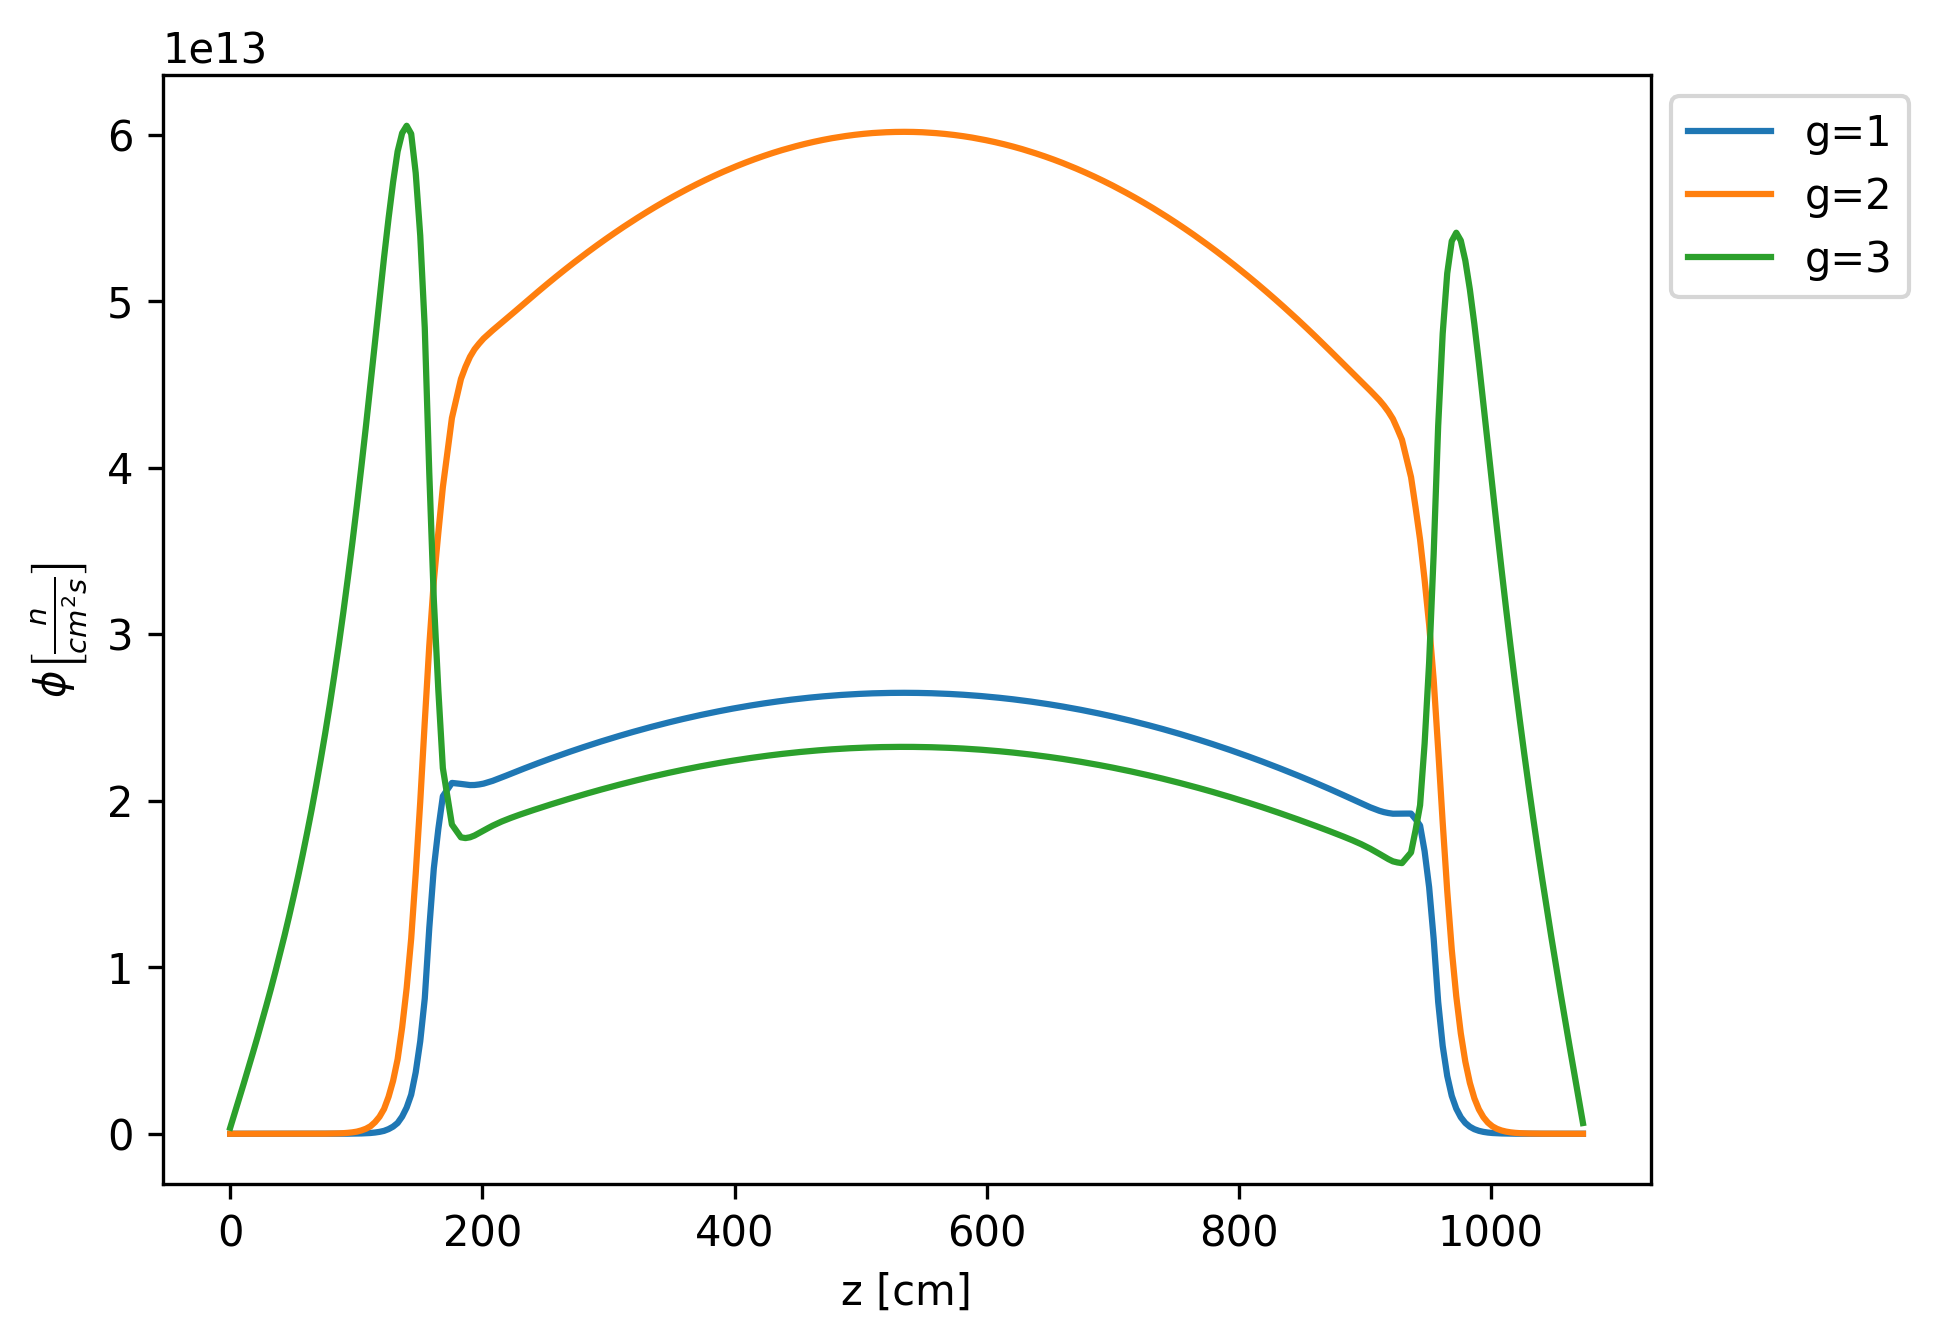
\includegraphics[width=0.45\textwidth]{figures-neutronics/3D-assembly-noLBP-600-26G}
    }
	\hfill
  \caption{Operational case 1: fuel column with no burnable poisons at 600K. Comparison of Serpent and Moltres-derived 3-group axial neutron fluxes.}
	\label{fig:assembly-noLBP-600-flux}
\end{figure}

% No LBP 1200
\begin{figure}[htbp!]
  \centering
    \subfloat[Serpent neutron flux.]{
        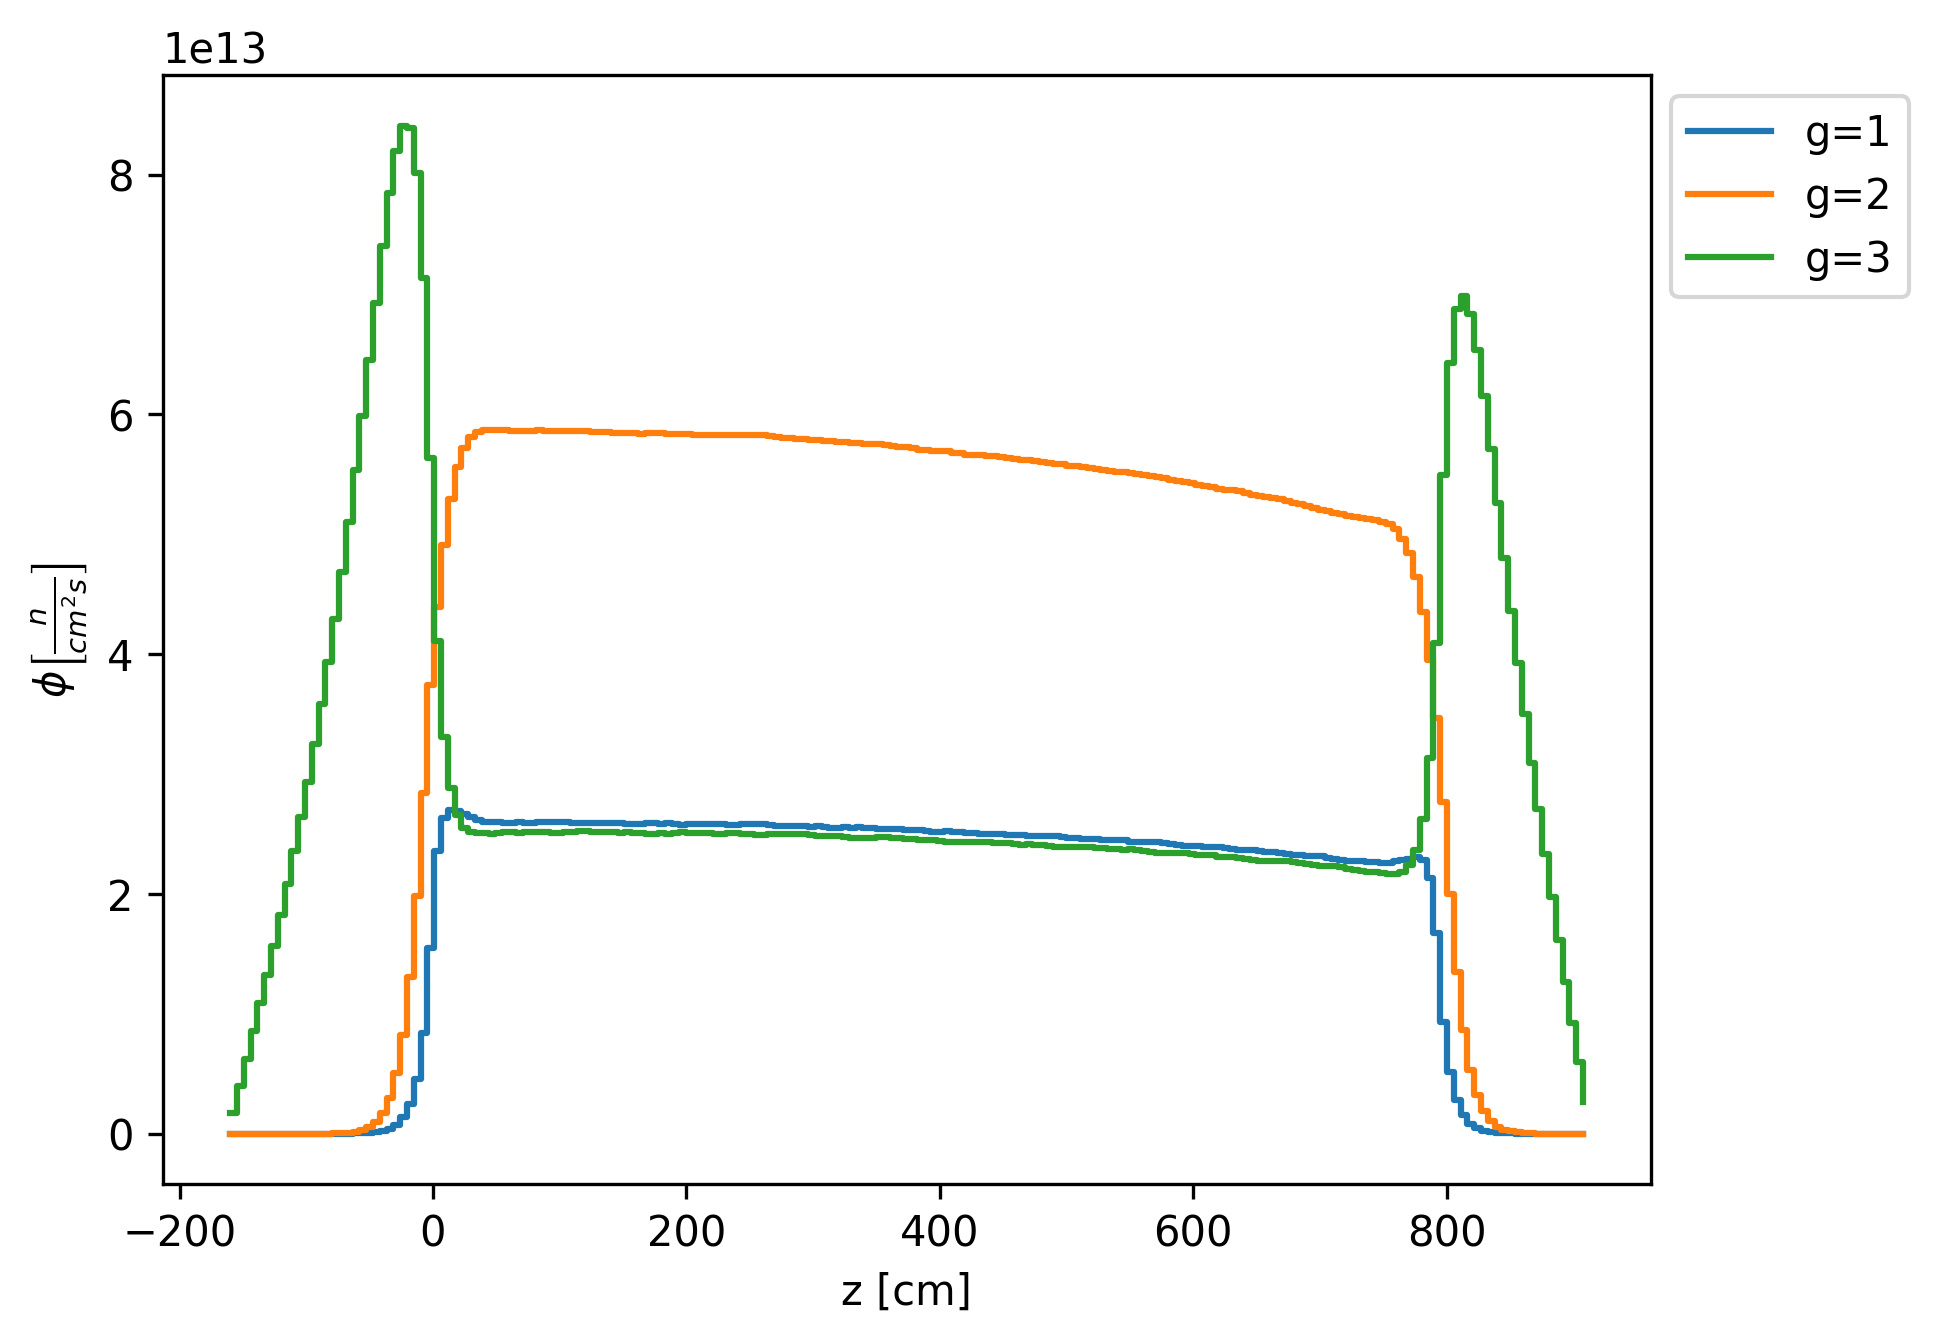
\includegraphics[width=0.45\textwidth]{figures-neutronics/serpent26G-noLBP-1200-collapse}
    }
    \subfloat[Moltres neutron flux.]{
        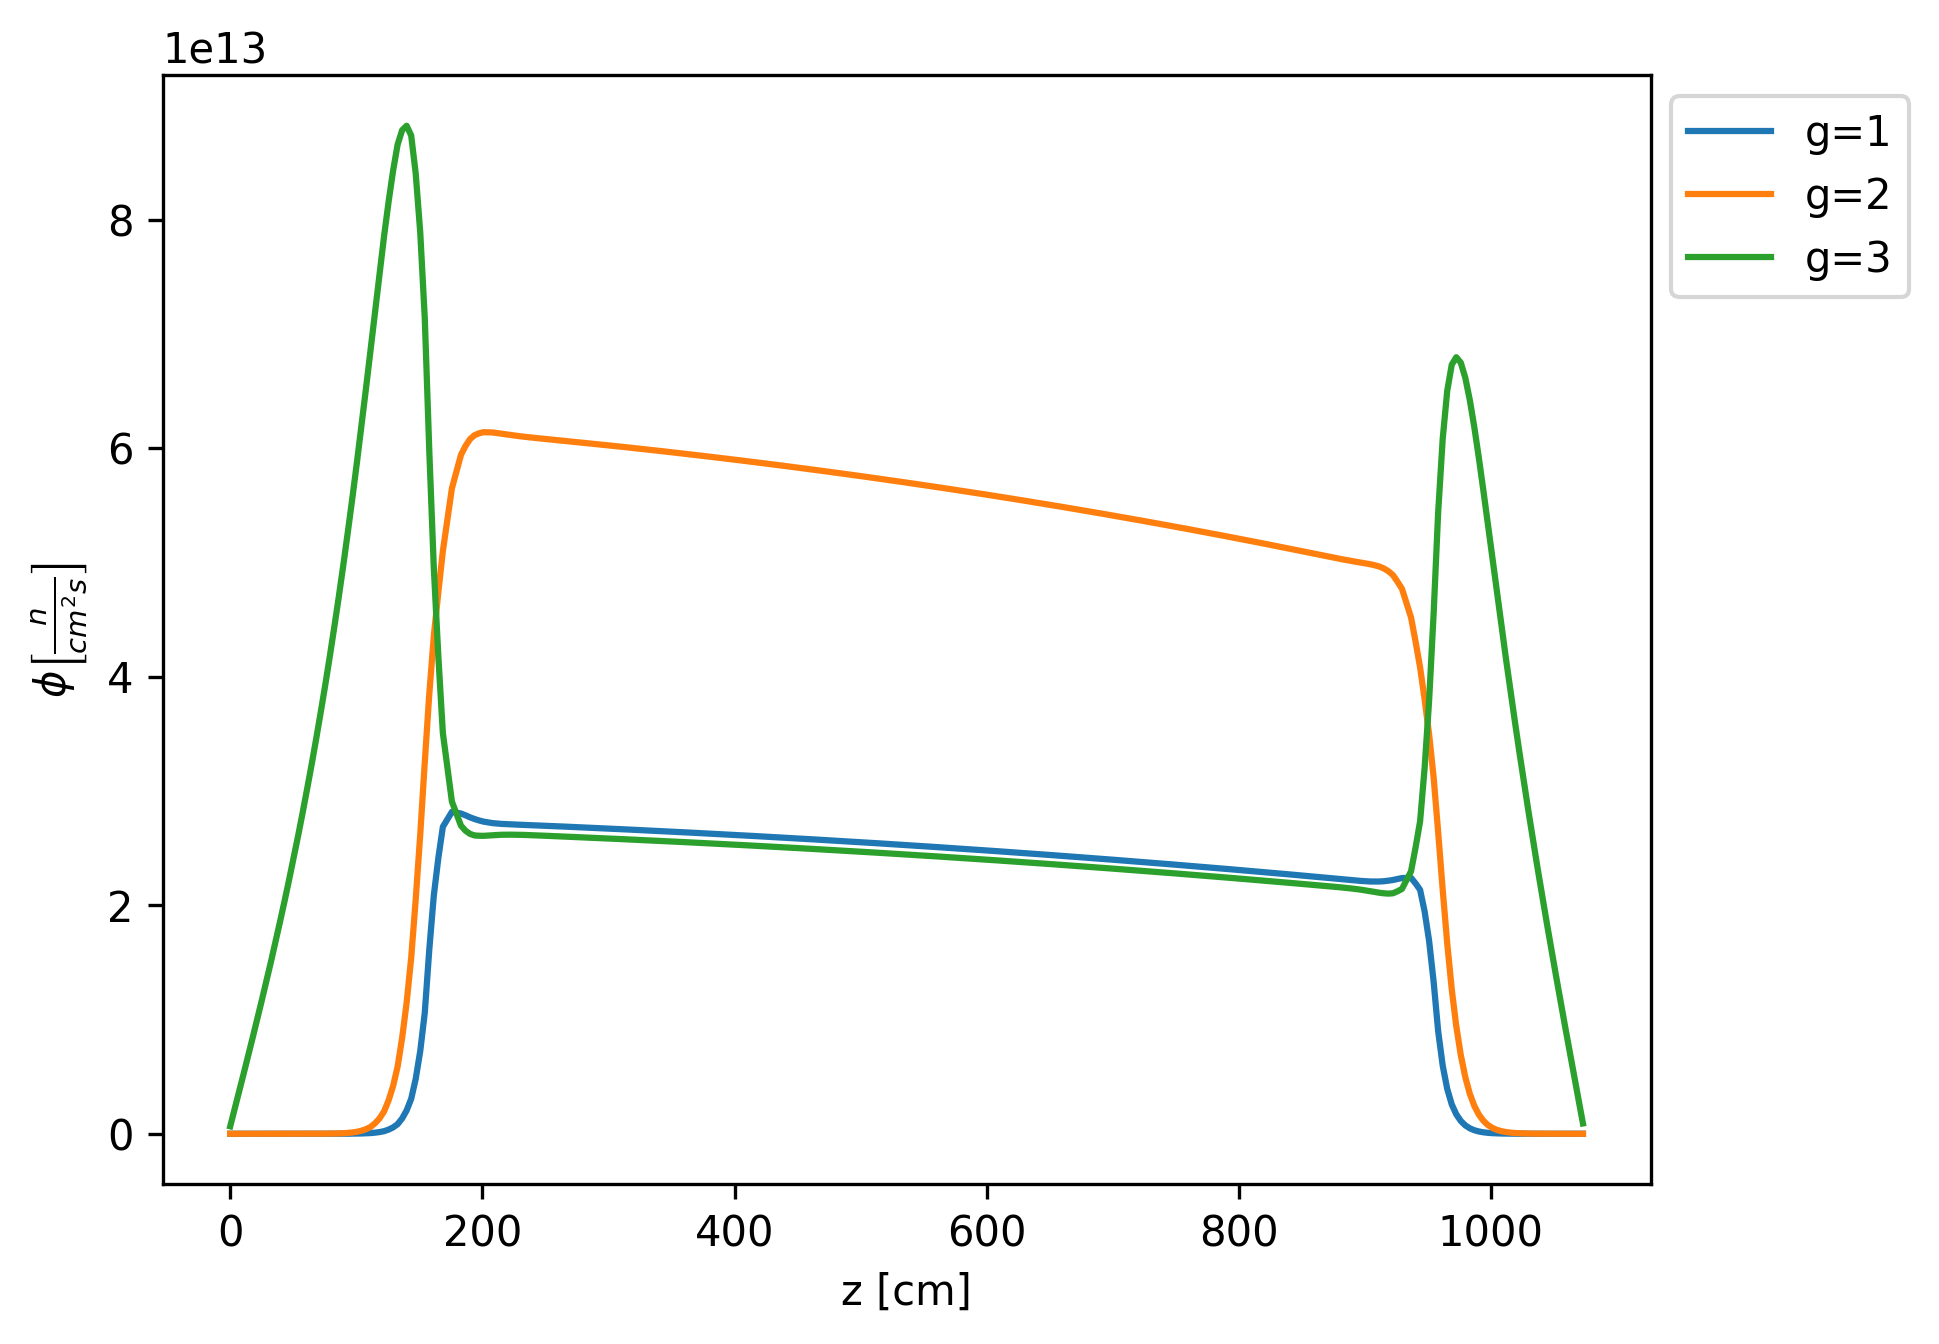
\includegraphics[width=0.45\textwidth]{figures-neutronics/3D-assembly-noLBP-1200-26G}
    }
  \hfill
  \caption{Operational case 2: fuel column with no burnable poisons at 1200K. Comparison of Serpent and Moltres-derived 3-group axial neutron fluxes.}
  \label{fig:assembly-noLBP-1200-flux}
\end{figure}

% LBP 600 
\begin{figure}[htbp!]
  \centering
    \subfloat[Serpent neutron flux.]{
        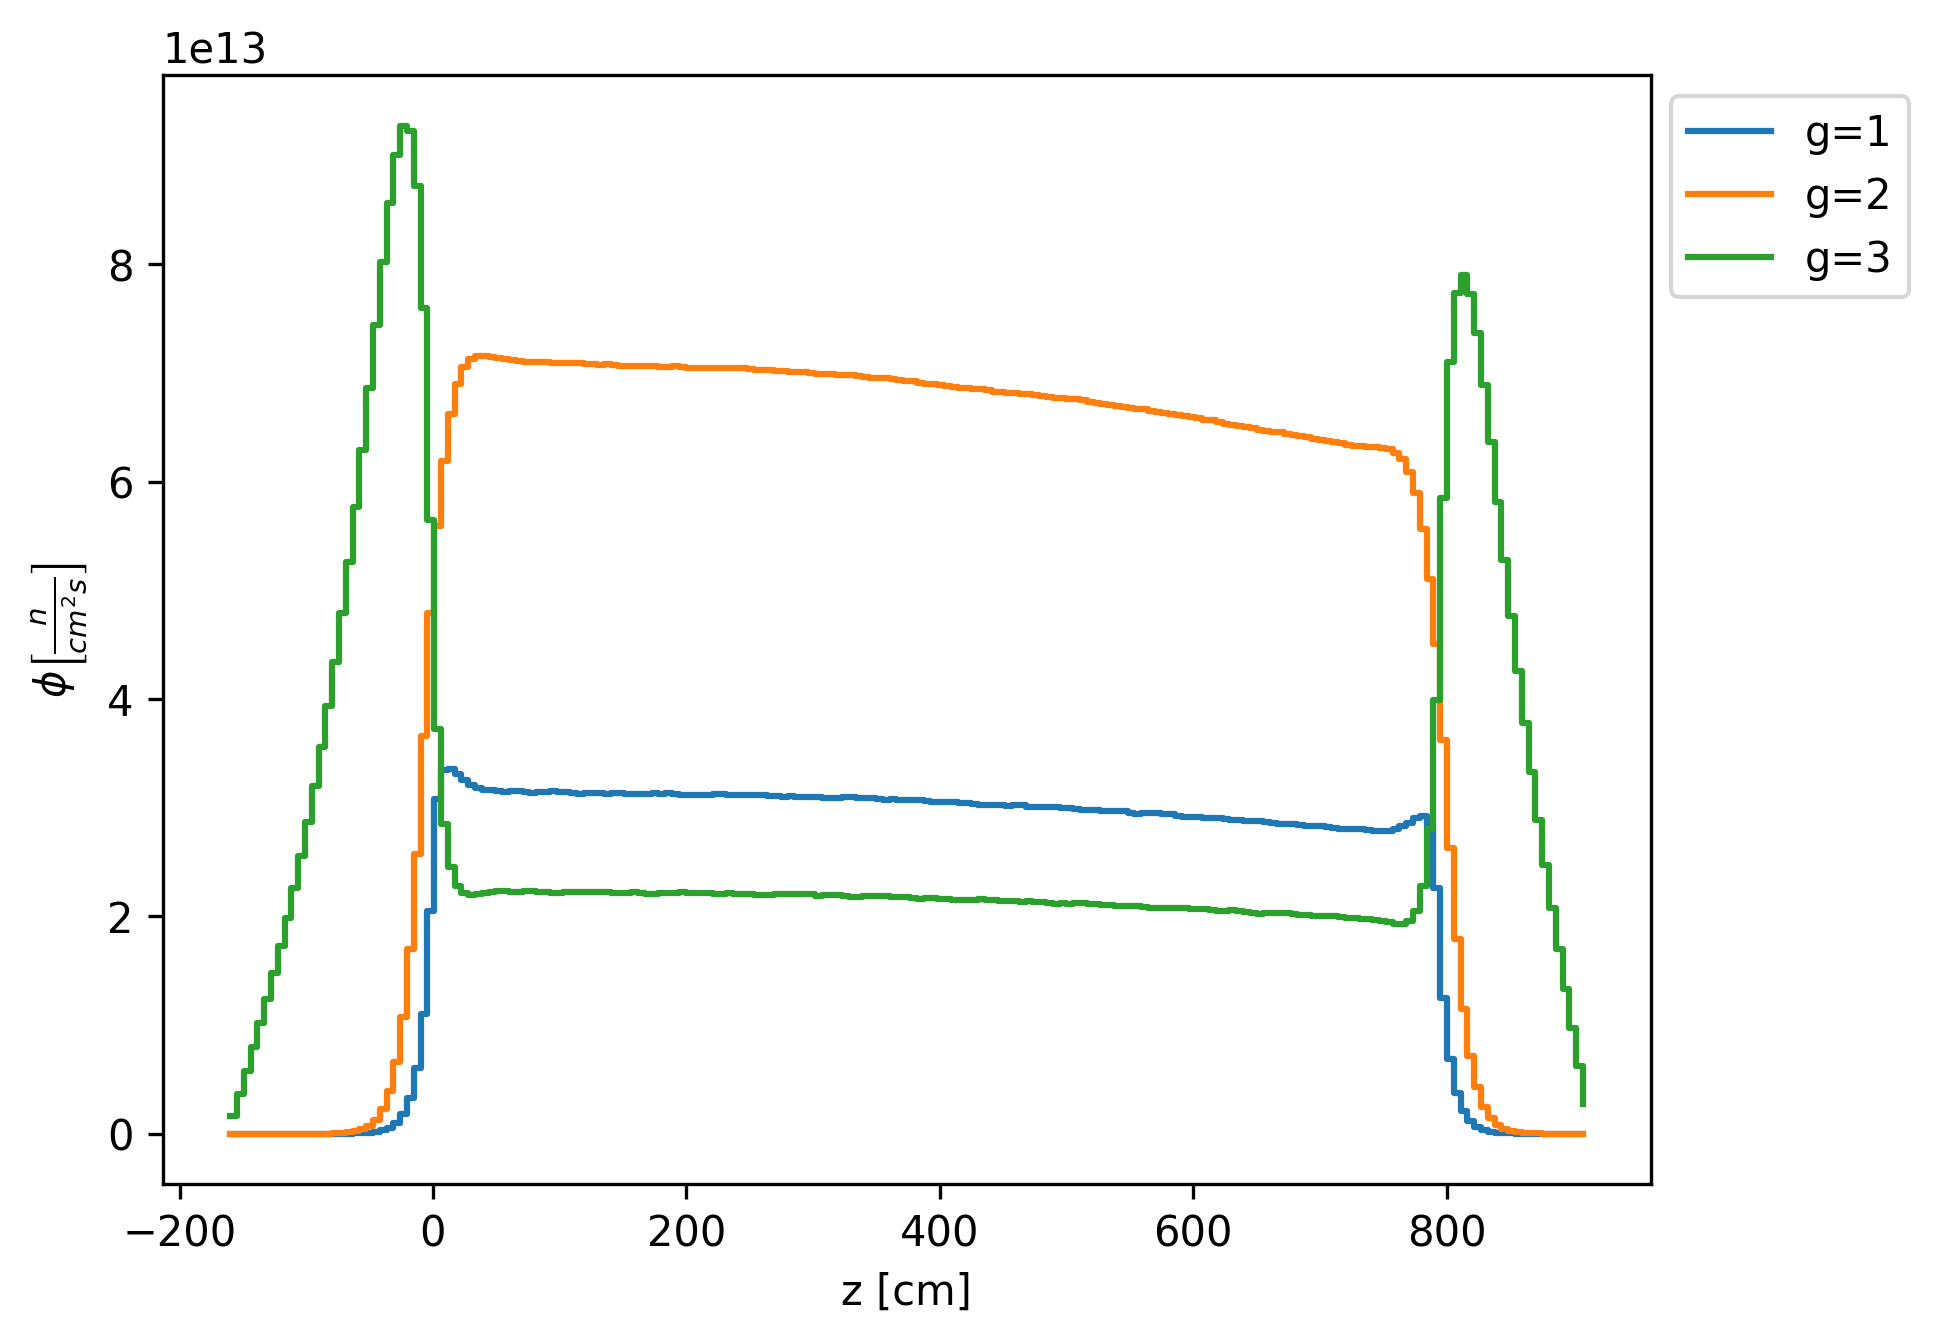
\includegraphics[width=0.45\textwidth]{figures-neutronics/serpent26G-LBP-600-collapse}
    }
    \subfloat[Moltres neutron flux.]{
        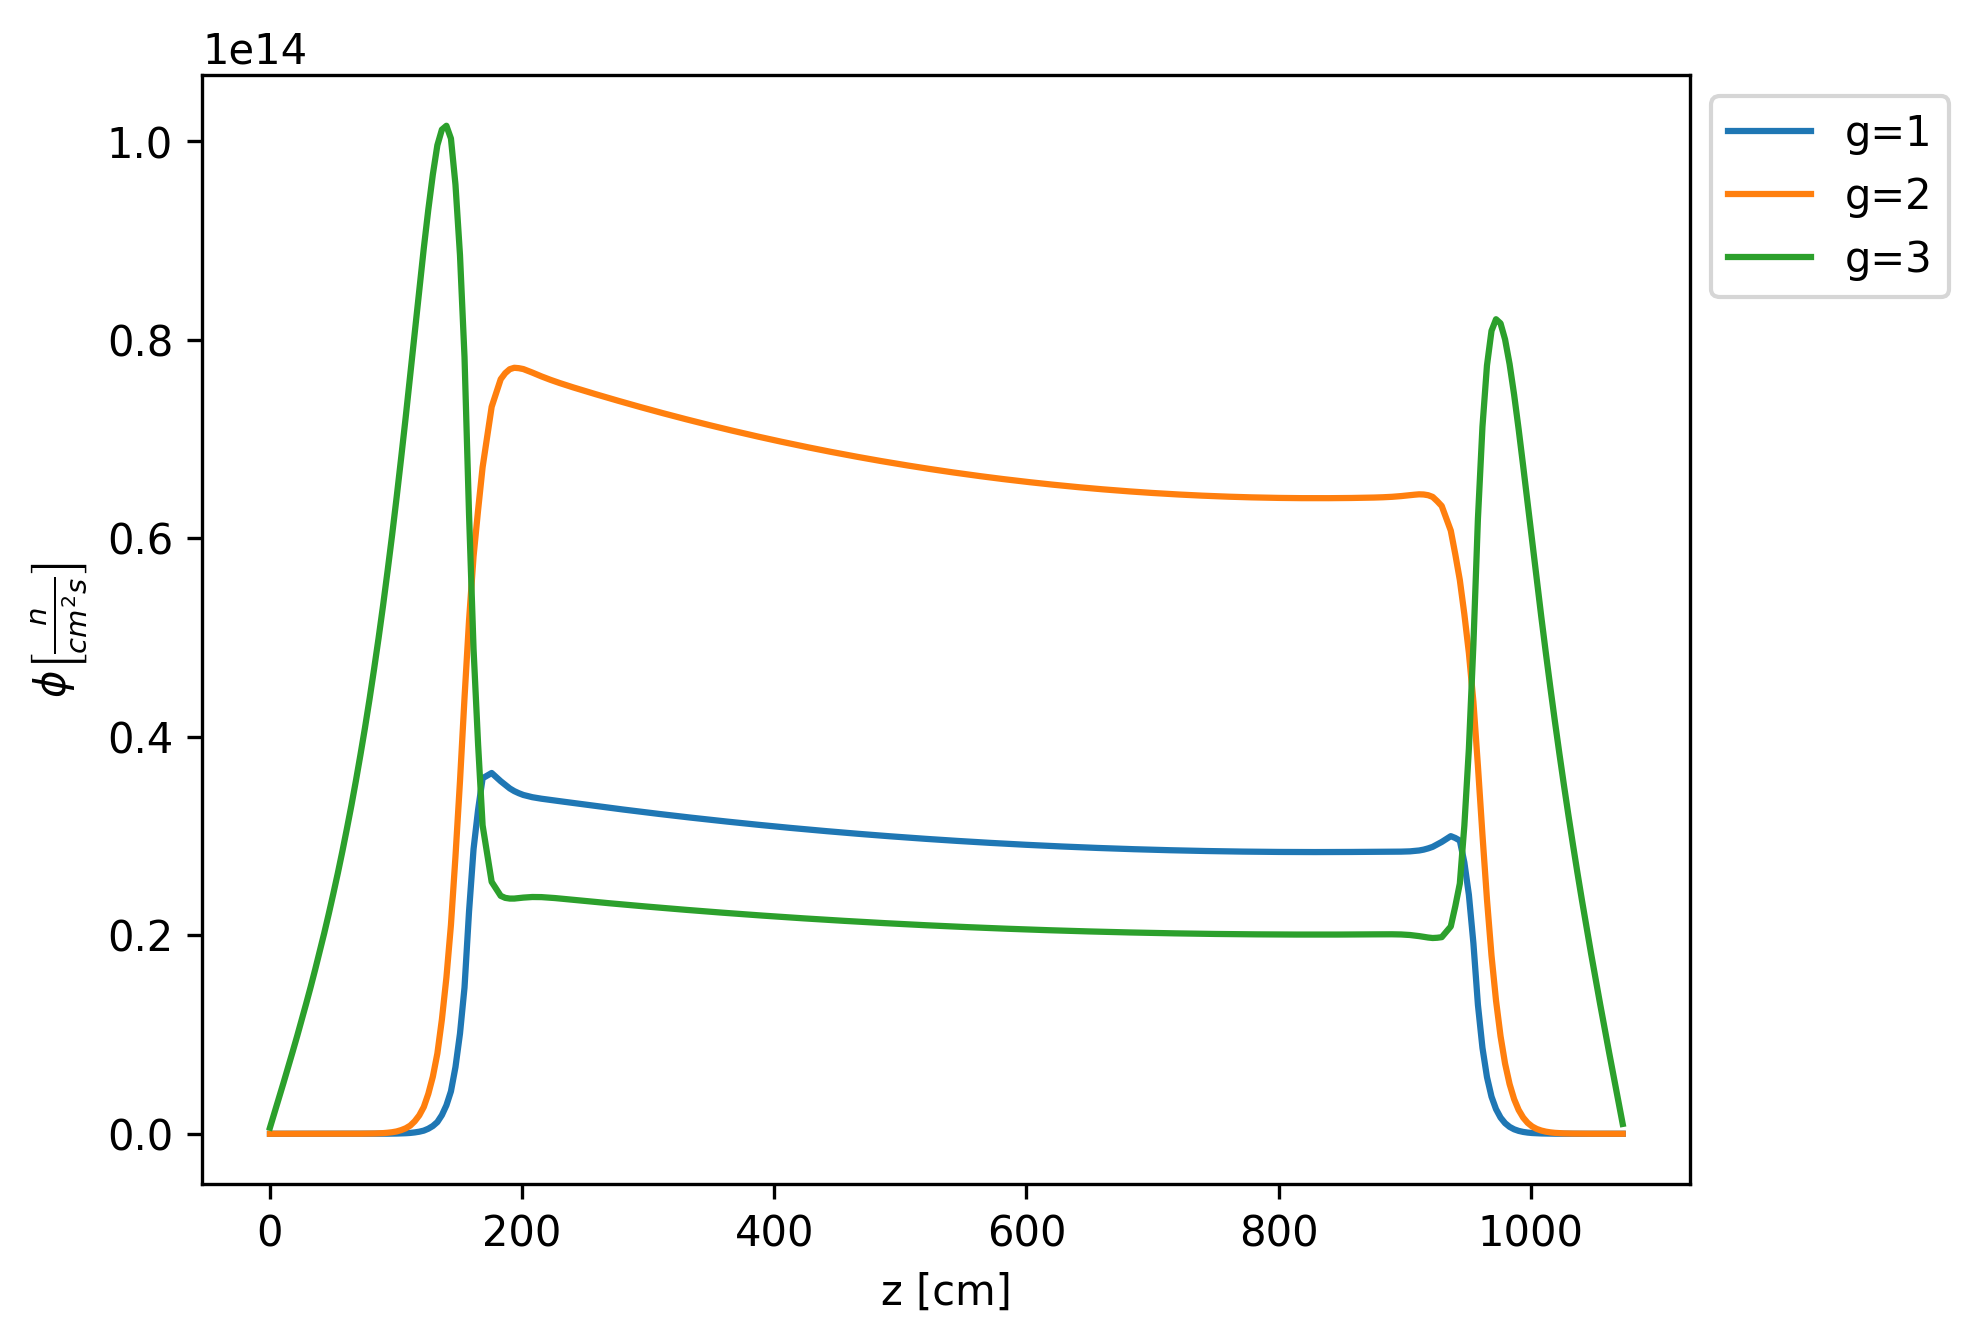
\includegraphics[width=0.45\textwidth]{figures-neutronics/3D-assembly-LBP-600-26G}
    }
  \hfill
  \caption{Operational case 3: fuel column with burnable poisons at 600K. Comparison of Serpent and Moltres-derived 3-group axial neutron fluxes.}
  \label{fig:assembly-LBP-600-flux}
\end{figure}

% LBP 1200
\begin{figure}[htbp!]
  \centering
    \subfloat[Serpent neutron flux.]{
        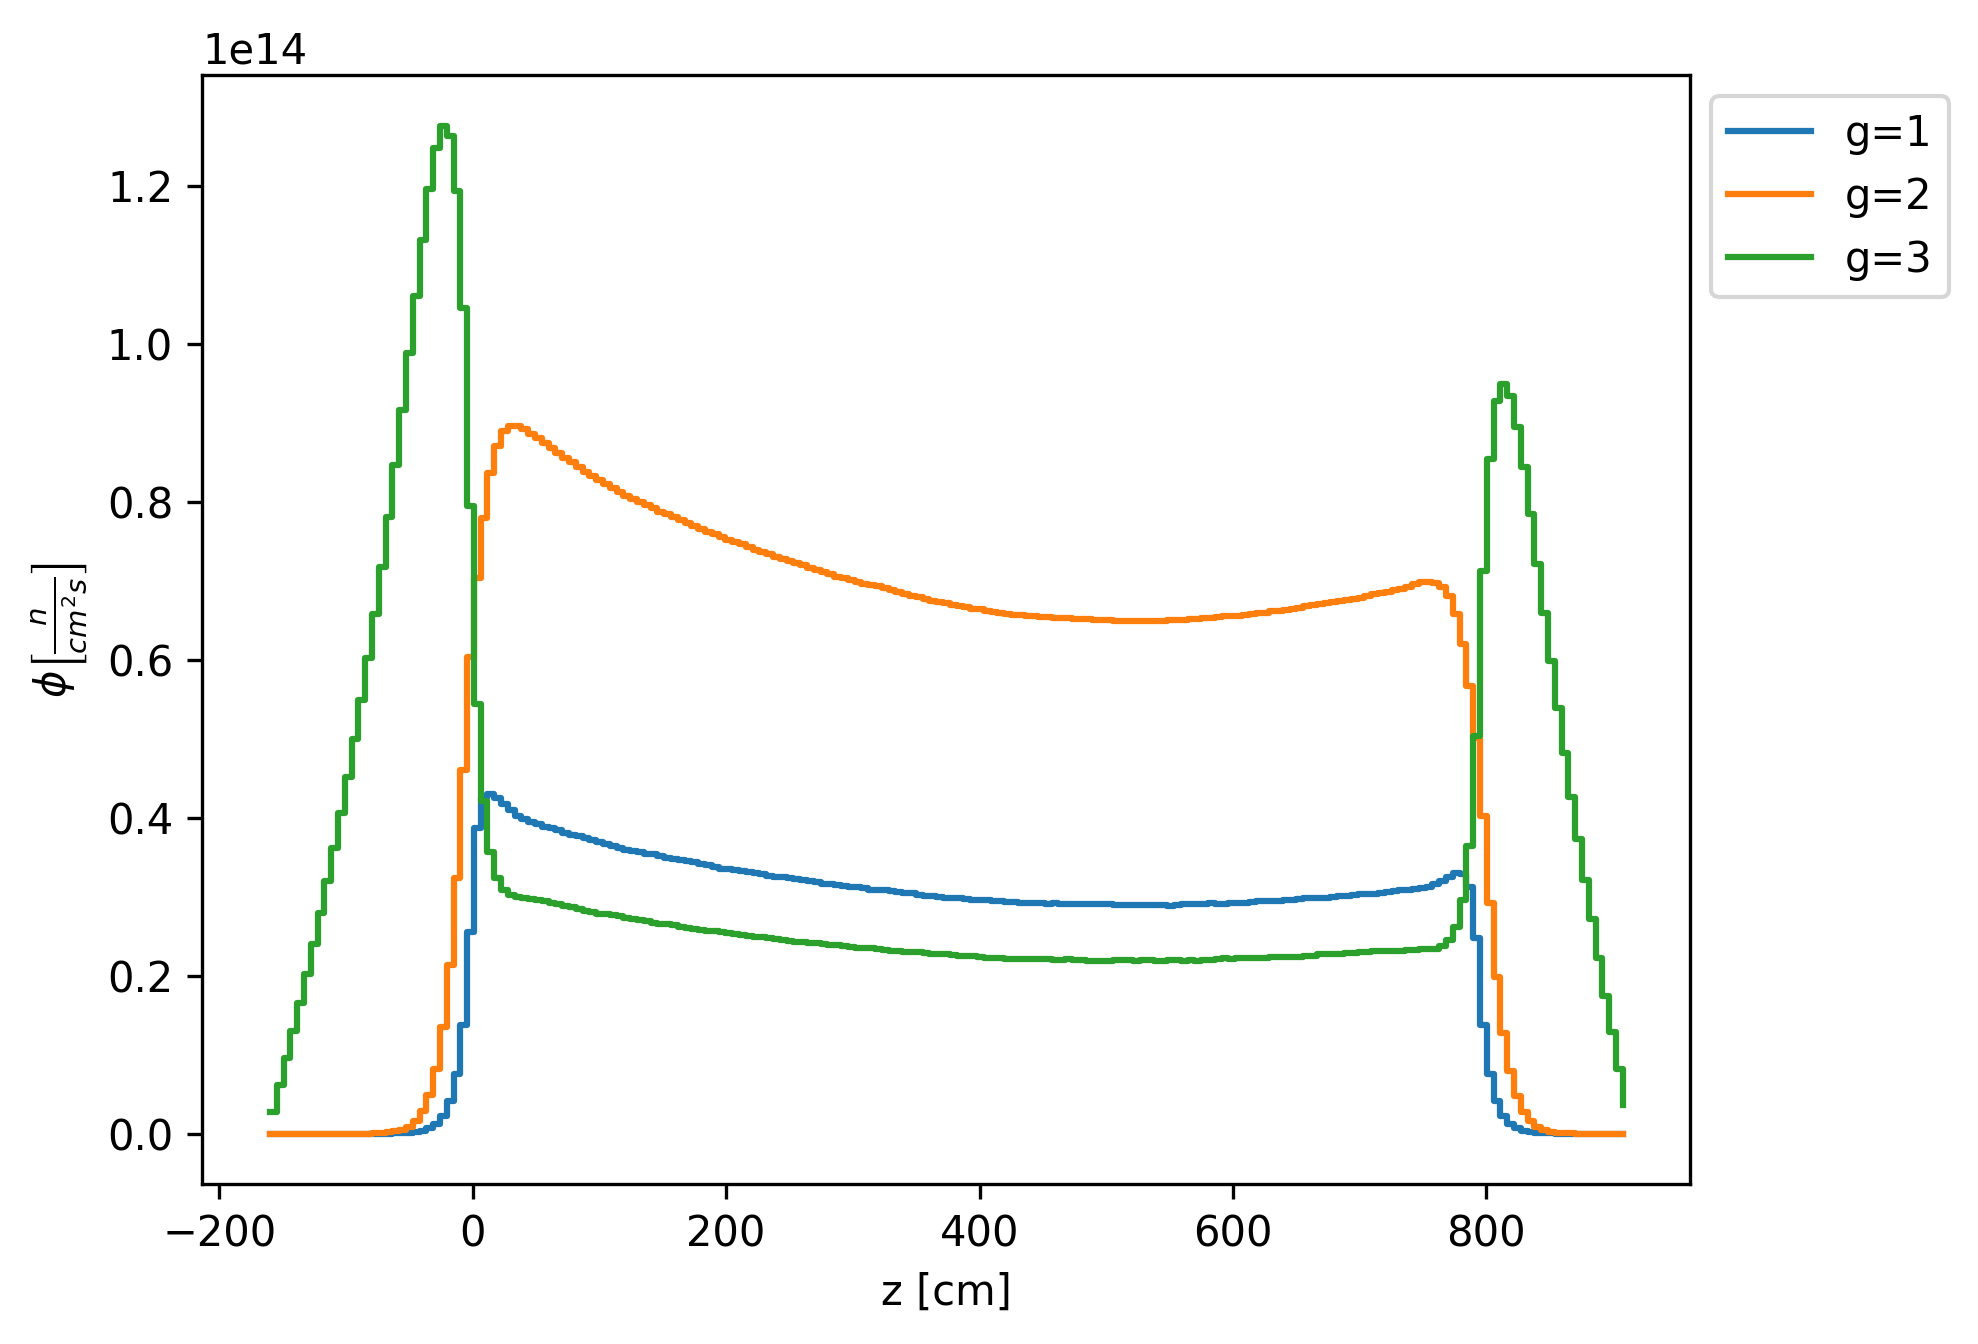
\includegraphics[width=0.45\textwidth]{figures-neutronics/serpent26G-LBP-1200-collapse}
    }
    \subfloat[Moltres neutron flux.]{
        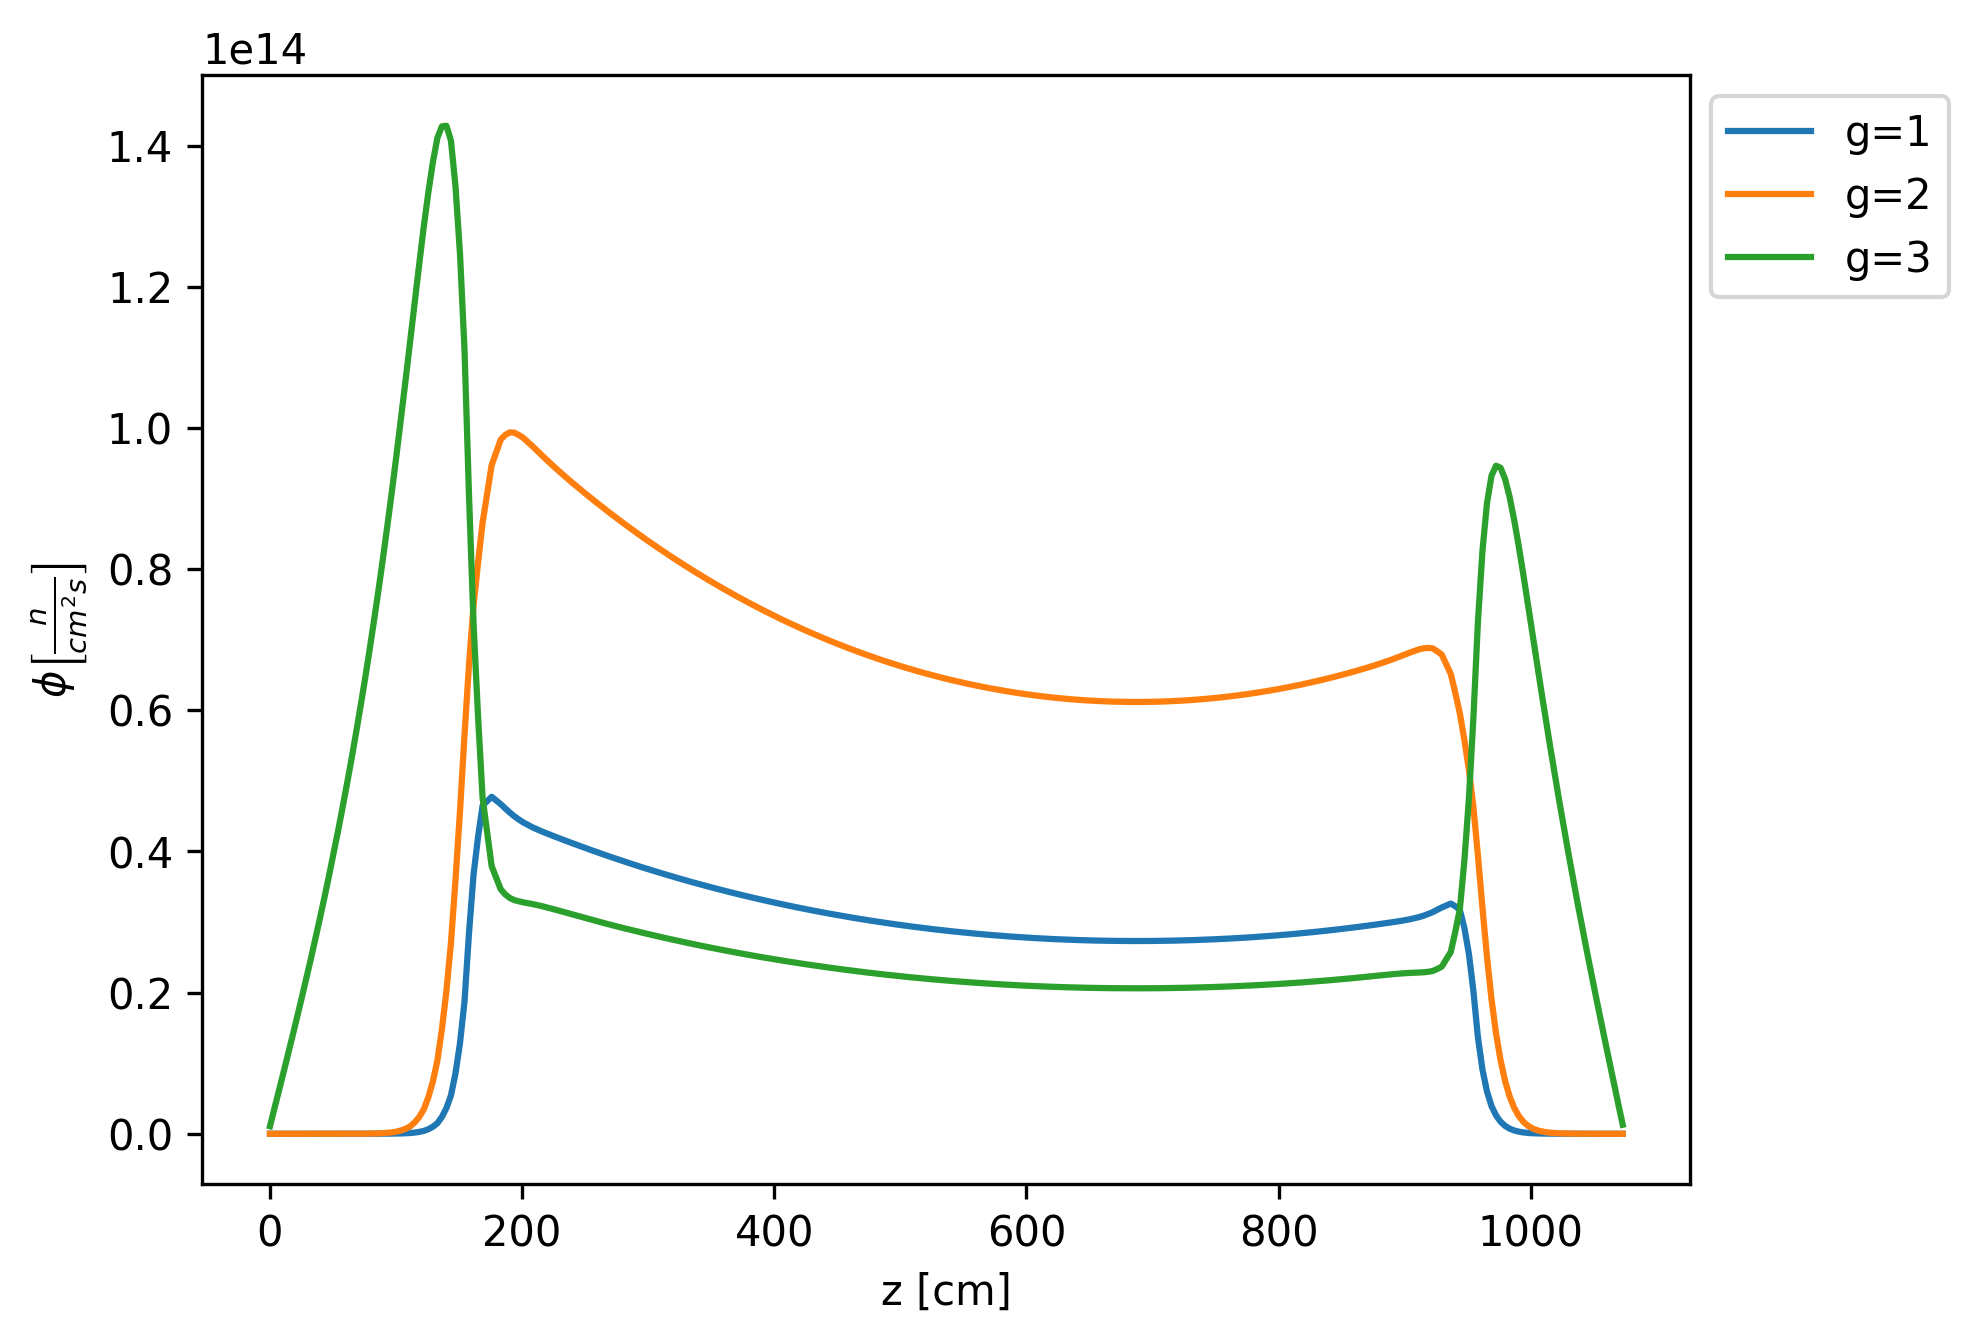
\includegraphics[width=0.45\textwidth]{figures-neutronics/3D-assembly-LBP-1200-26G}
    }
  \hfill
  \caption{Operational case 4: fuel column with burnable poisons at 1200K. Comparison of Serpent and Moltres-derived 3-group axial neutron fluxes.}
  \label{fig:assembly-LBP-1200-flux}
\end{figure}

% eigenvalues
Equation \ref{eq:delta-rho} calculates the reactivity difference ($\Delta \rho$) between the eigenvalues calculated by Serpent and Moltres
\begin{align}
	& \Delta \rho = \left| \rho_1 - \rho_2 \right| = \left| \frac{k_1-1}{k_1} - \frac{k_2-1}{k_2} \right| = \left| \frac{k_1-k_2}{k_1 k_2} \right| \label{eq:delta-rho} \\
  \intertext{where}
  & k_1 = \mbox{Serpent-derived eigenvalue} [-] \notag \\
  & k_2 = \mbox{Moltres-derived eigenvalue} [-]. \notag
\end{align}

Table \ref{tab:keff} exhibits the eigenvalues calculated by Serpent and $\Delta \rho$ for the different energy group structures.
The eigenvalues in Moltres differ slightly from the eigenvalues in Serpent, and overall, the reactivity difference is less than 50 pcm.
The number of energy groups does not affect the accuracy of the eigenvalue calculations in Moltres.

\begin{table}[htbp!]
  \centering
  \caption{Eigenvalues calculated by Serpent and reactivity difference between eigenvalues calculated by Moltres and Serpent, see equation \ref{eq:delta-rho}, for the different energy group structures.}
  \begin{tabular}{c|c|cccccccc}
  \toprule
Operational case  & Serpent       & \multicolumn{8}{c}{$\Delta \rho$ [pcm]}            \\ \cline{3-10} 
                  & eigenvalues   & 3   & 6   & 9   & 12   & 15   & 18   & 21   & 26   \\
  \midrule
1 & 1.43800 $\pm$ 0.00008 & 10  & 7   & 6   & 6    & 5    & 6    & 6    & 12   \\
2 & 1.37771 $\pm$ 0.00008 & 23  & 15  & 4   & 3    & 2    & 2    & 1    & 11   \\
3 & 1.12861 $\pm$ 0.00009 & 44  & 21  & 24  & 25   & 25   & 24   & 19   & 9    \\
4 & 1.06554 $\pm$ 0.00010 & 36  & 40  & 29  & 32   & 44   & 43   & 25   & 25   \\
  \bottomrule
  \end{tabular}
  \label{tab:keff}
\end{table}

The last analysis is for the Moltres axial flux.
Considering the 26 group structure as the reference value, equation \ref{eq:l2norm} obtained the $L_2$-norm of the active core's axial flux relative difference
\begin{align}
  & \Delta_{L_2} = \left\| \frac{\phi_G(z)-\phi_{ref}(z)}{\phi_{ref}(z)} \right\|  \quad \wedge \quad z\quad \in \quad L_a \label{eq:l2norm}
  \intertext{where}
  & \Delta_{L_2} = \mbox{L$_2$-norm relative difference } [-] \notag \\
  & \phi_G(z) = \mbox{$G$-energy groups axial flux } [n \cdot cm^{-2} \cdot s^{-1}] \notag \\
  & \phi_{ref}(z) = \mbox{reference axial flux } [n \cdot cm^{-2} \cdot s^{-1}] \notag \\
  & L_a = \mbox{active core length } [cm]. \notag
\end{align}

Figures \ref{fig:assembly-noLBP-er} and \ref{fig:assembly-LBP-er} show $\Delta_{L_2}$ for the various energy group structures.
Overall, the relative error decreases with an increase in the number of energy groups.
Nonetheless, this is not always the case.
For example, in Figure \ref{fig:assembly-noLBP-er-b}, from 12 to 15-energy groups, the thermal flux agreement improves, but the fast flux agreement worsens.
Additionally, the relative error of the cases with no burnable poisons is smaller than the relative error of the cases with burnable poison.
The treatment of the burnable poisons challenges the accuracy of the homogenized simulations in Moltres.
For example, a three-energy group structure yields more than 100$\%$ error when treating the burnable poison, Figure \ref{fig:assembly-LBP-er}.

% No LBP
\begin{figure}[htbp!]
	\centering
    \subfloat[Operational case 1: 600K.]{
        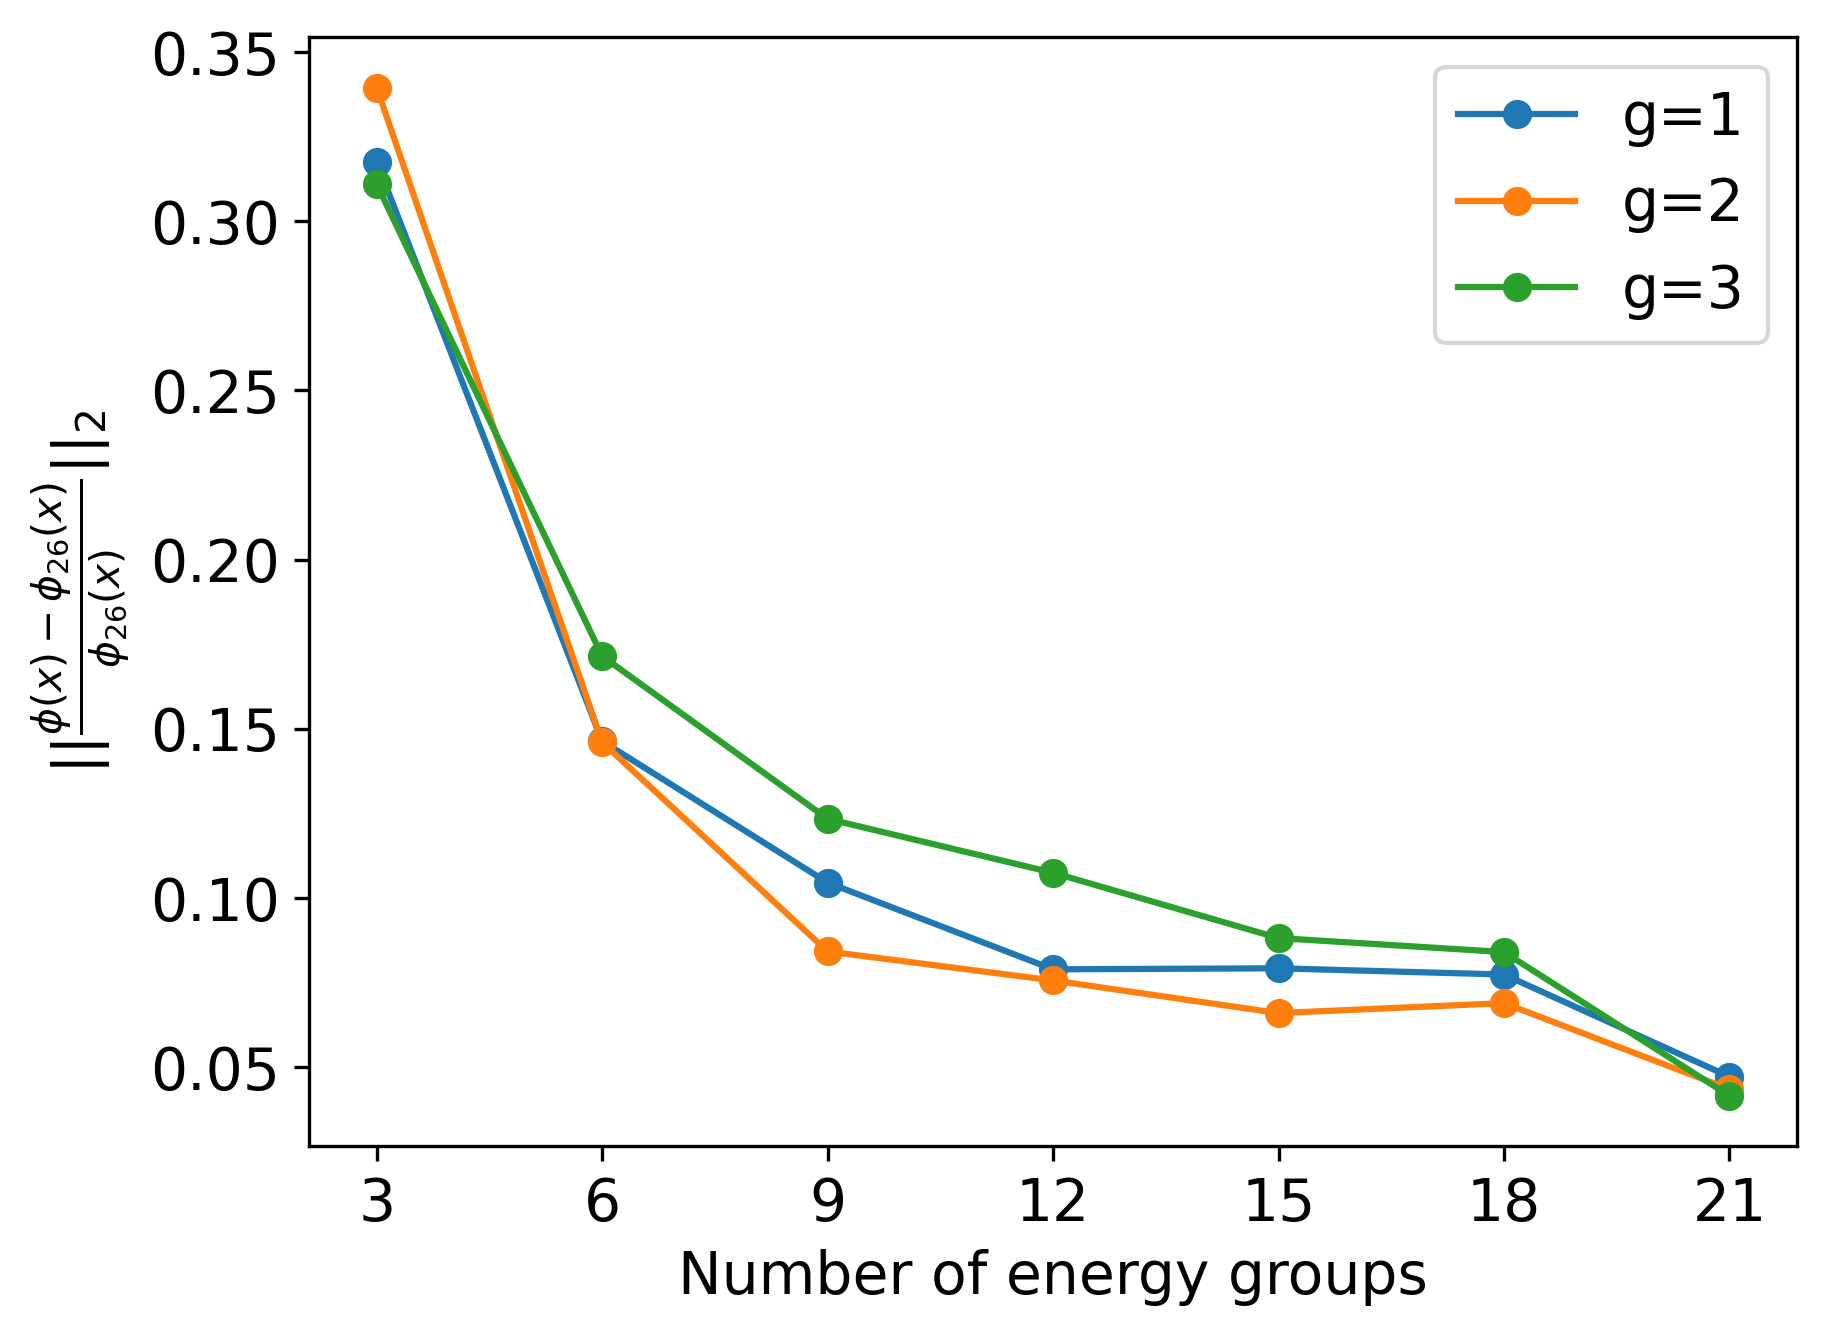
\includegraphics[width=0.45\textwidth]{figures-neutronics/noLBP-600-er-final}
    }
    \subfloat[Operational case 2: 1200K.\label{fig:assembly-noLBP-er-b}]{
        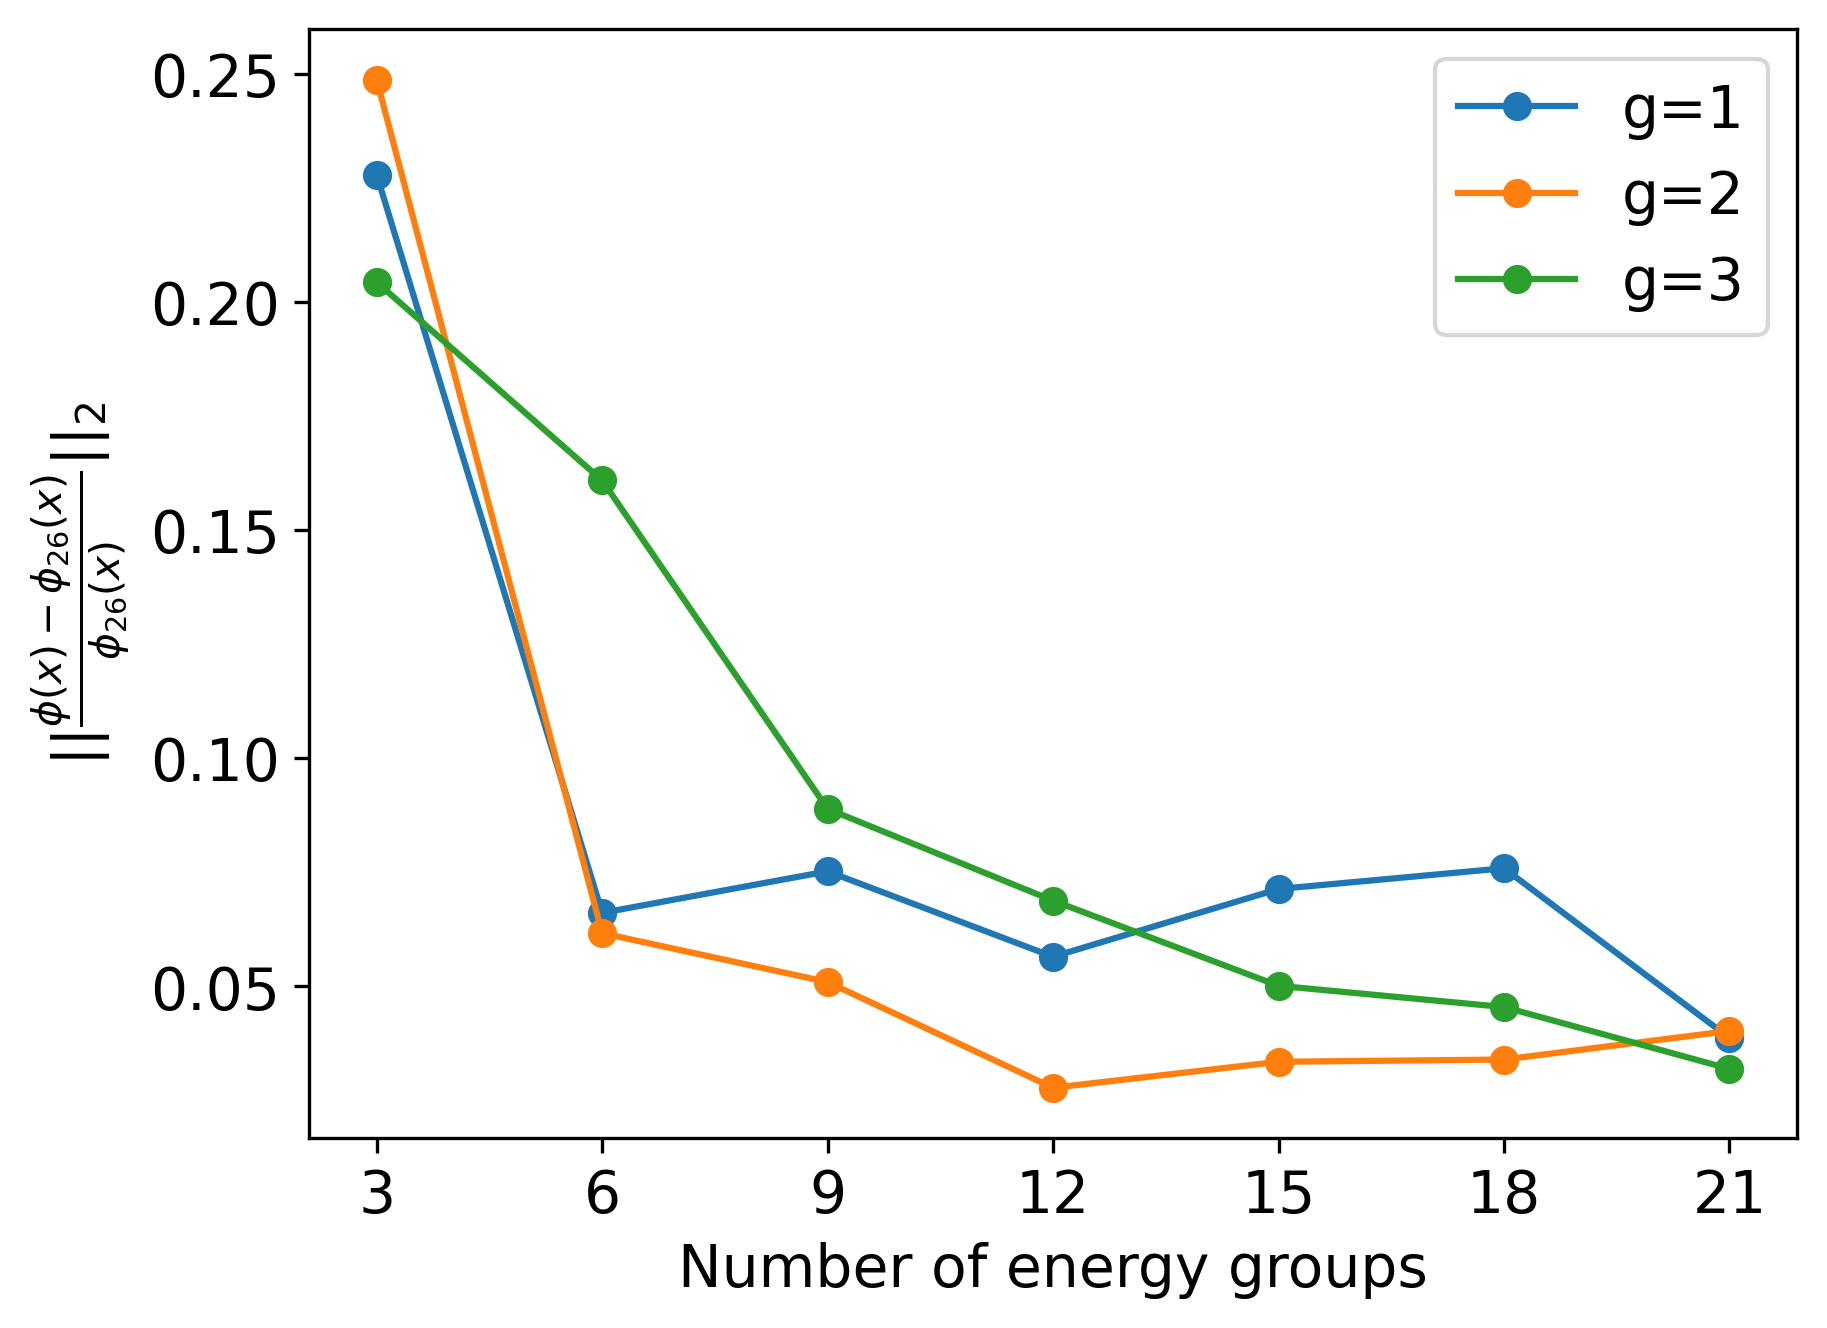
\includegraphics[width=0.45\textwidth]{figures-neutronics/noLBP-1200-er-final}
    }
	\hfill
    \caption{L$_2$-norm relative error for different number of energy group structures for the operational cases with no burnable poisons.}
	\label{fig:assembly-noLBP-er}
\end{figure}

% LBP
\begin{figure}[htbp!]
	\centering
    \subfloat[Operational case 3: 600K.]{
        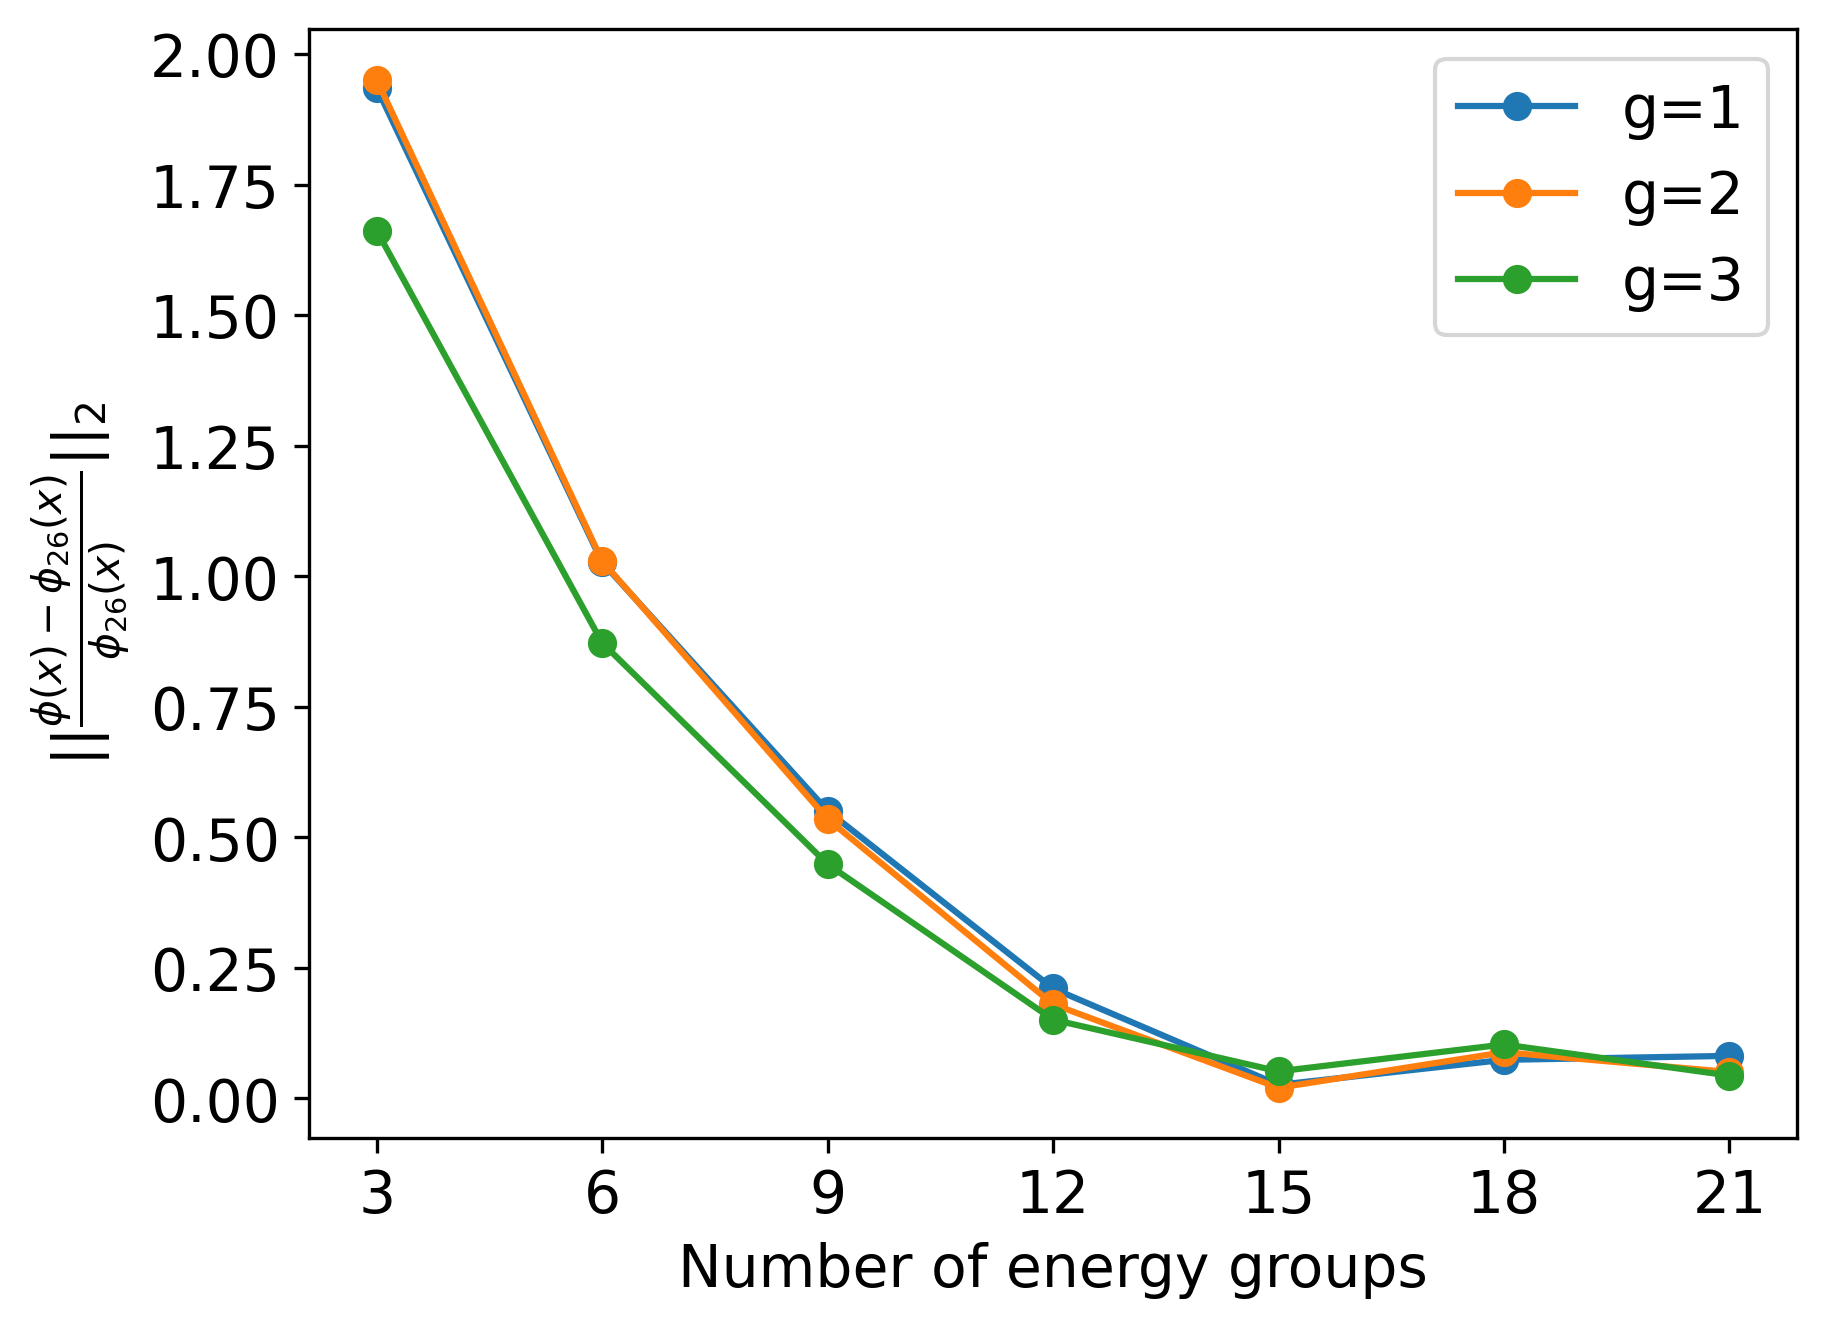
\includegraphics[width=0.45\textwidth]{figures-neutronics/LBP-600-er-final}
    }
    \subfloat[Operational case 4: 1200K.]{
        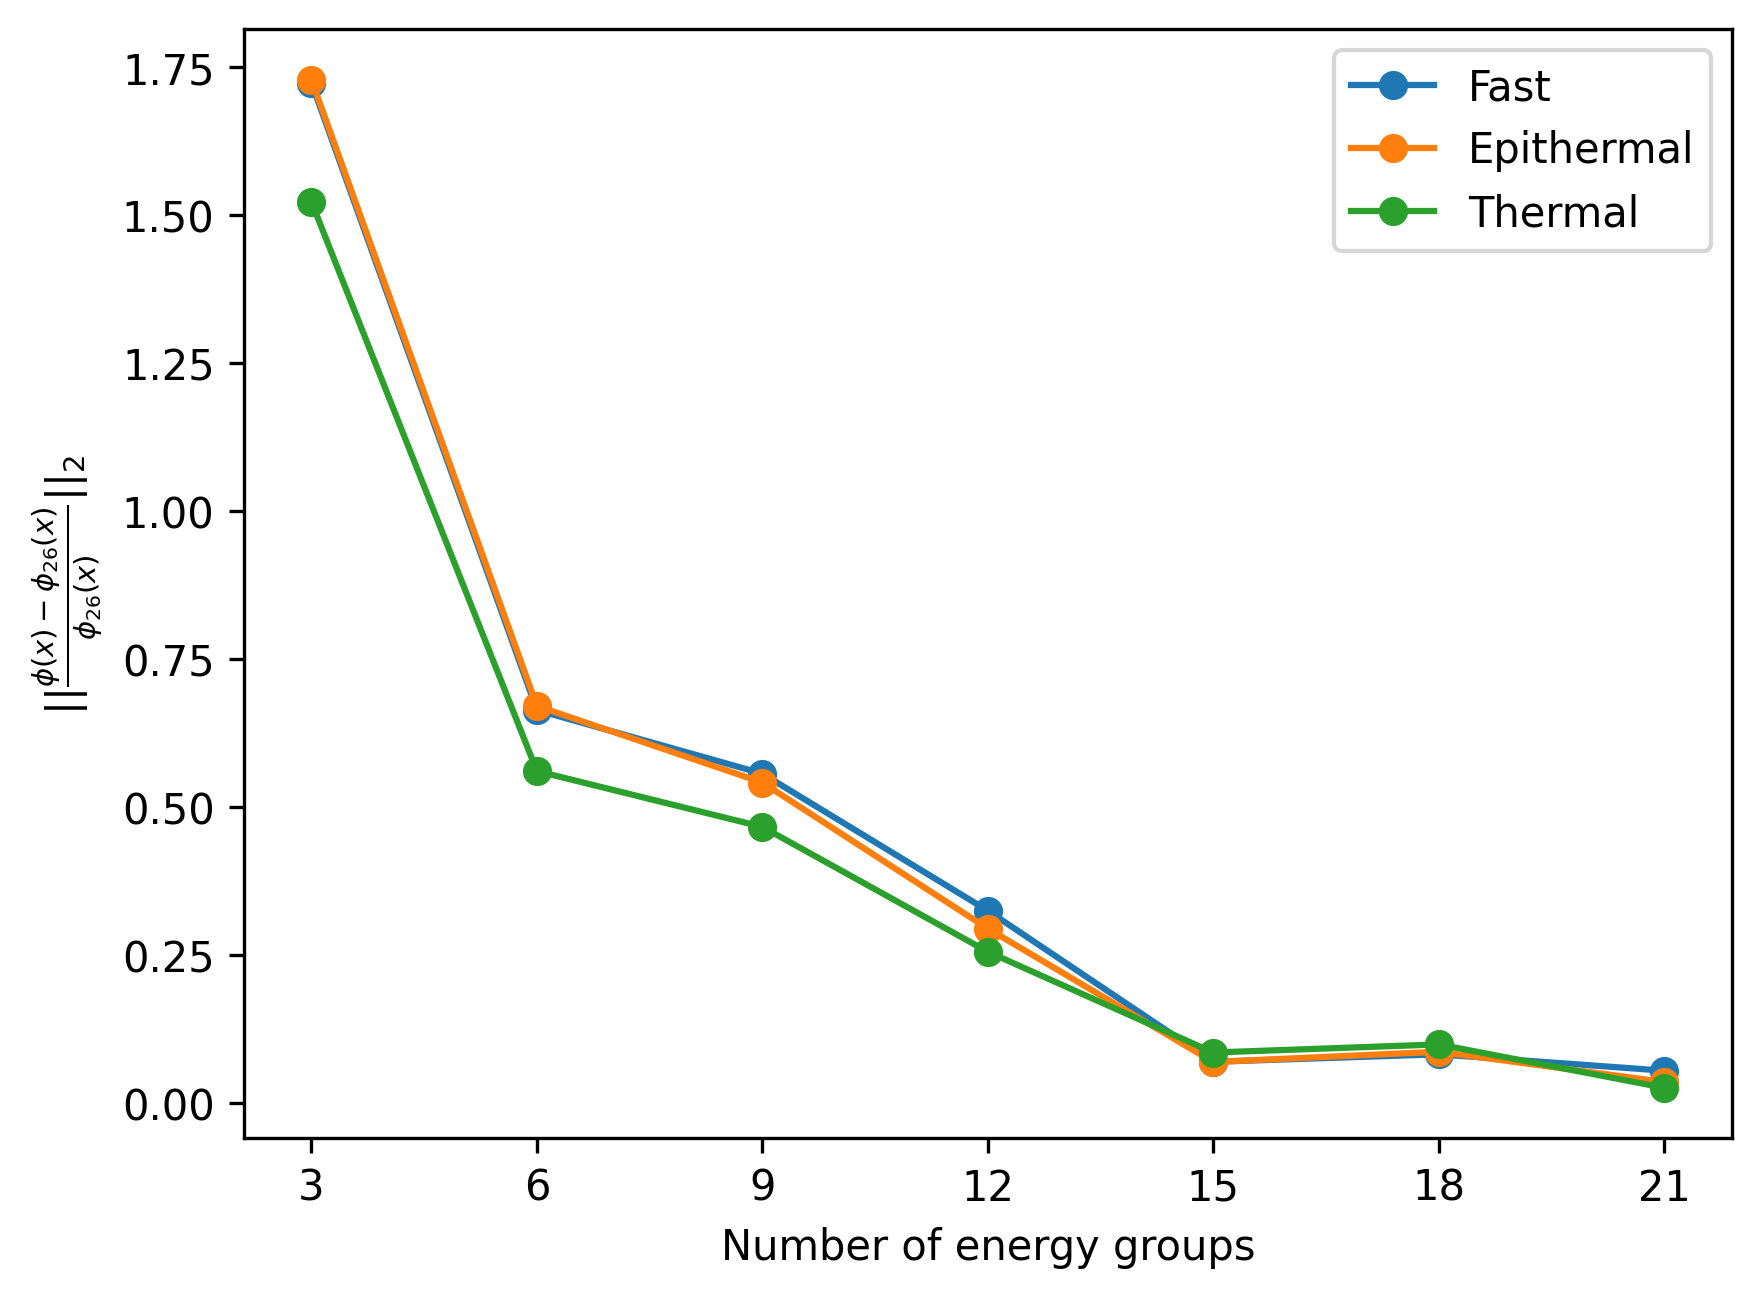
\includegraphics[width=0.45\textwidth]{figures-neutronics/LBP-1200-er-final}
    }
	\hfill
    \caption{LBP case. L$_2$-norm relative error for different number of energy group structures for the operational cases with burnable poisons.}
	\label{fig:assembly-LBP-er}
\end{figure}

The analysis also included the computational time and the peak memory usage during the simulations, as shown in Figure \ref{fig:assembly-time}.
All the simulations used 128 cores.
This section presents only the cases at 600K because the impact of the temperature change was not significant.
The computational requirements rise with an increase in the number of energy groups.
As the geometry uses a constant number of elements, the number of DoFs per energy-group remains constant for all the simulations.
Figure \ref{fig:assembly-time} also shows that the overall time of the cases with burnable poison is higher than the cases without them.

% Time and memory
\begin{figure}[htbp!]
	\centering
    \subfloat[No burnable poisons at 600 K.]{
        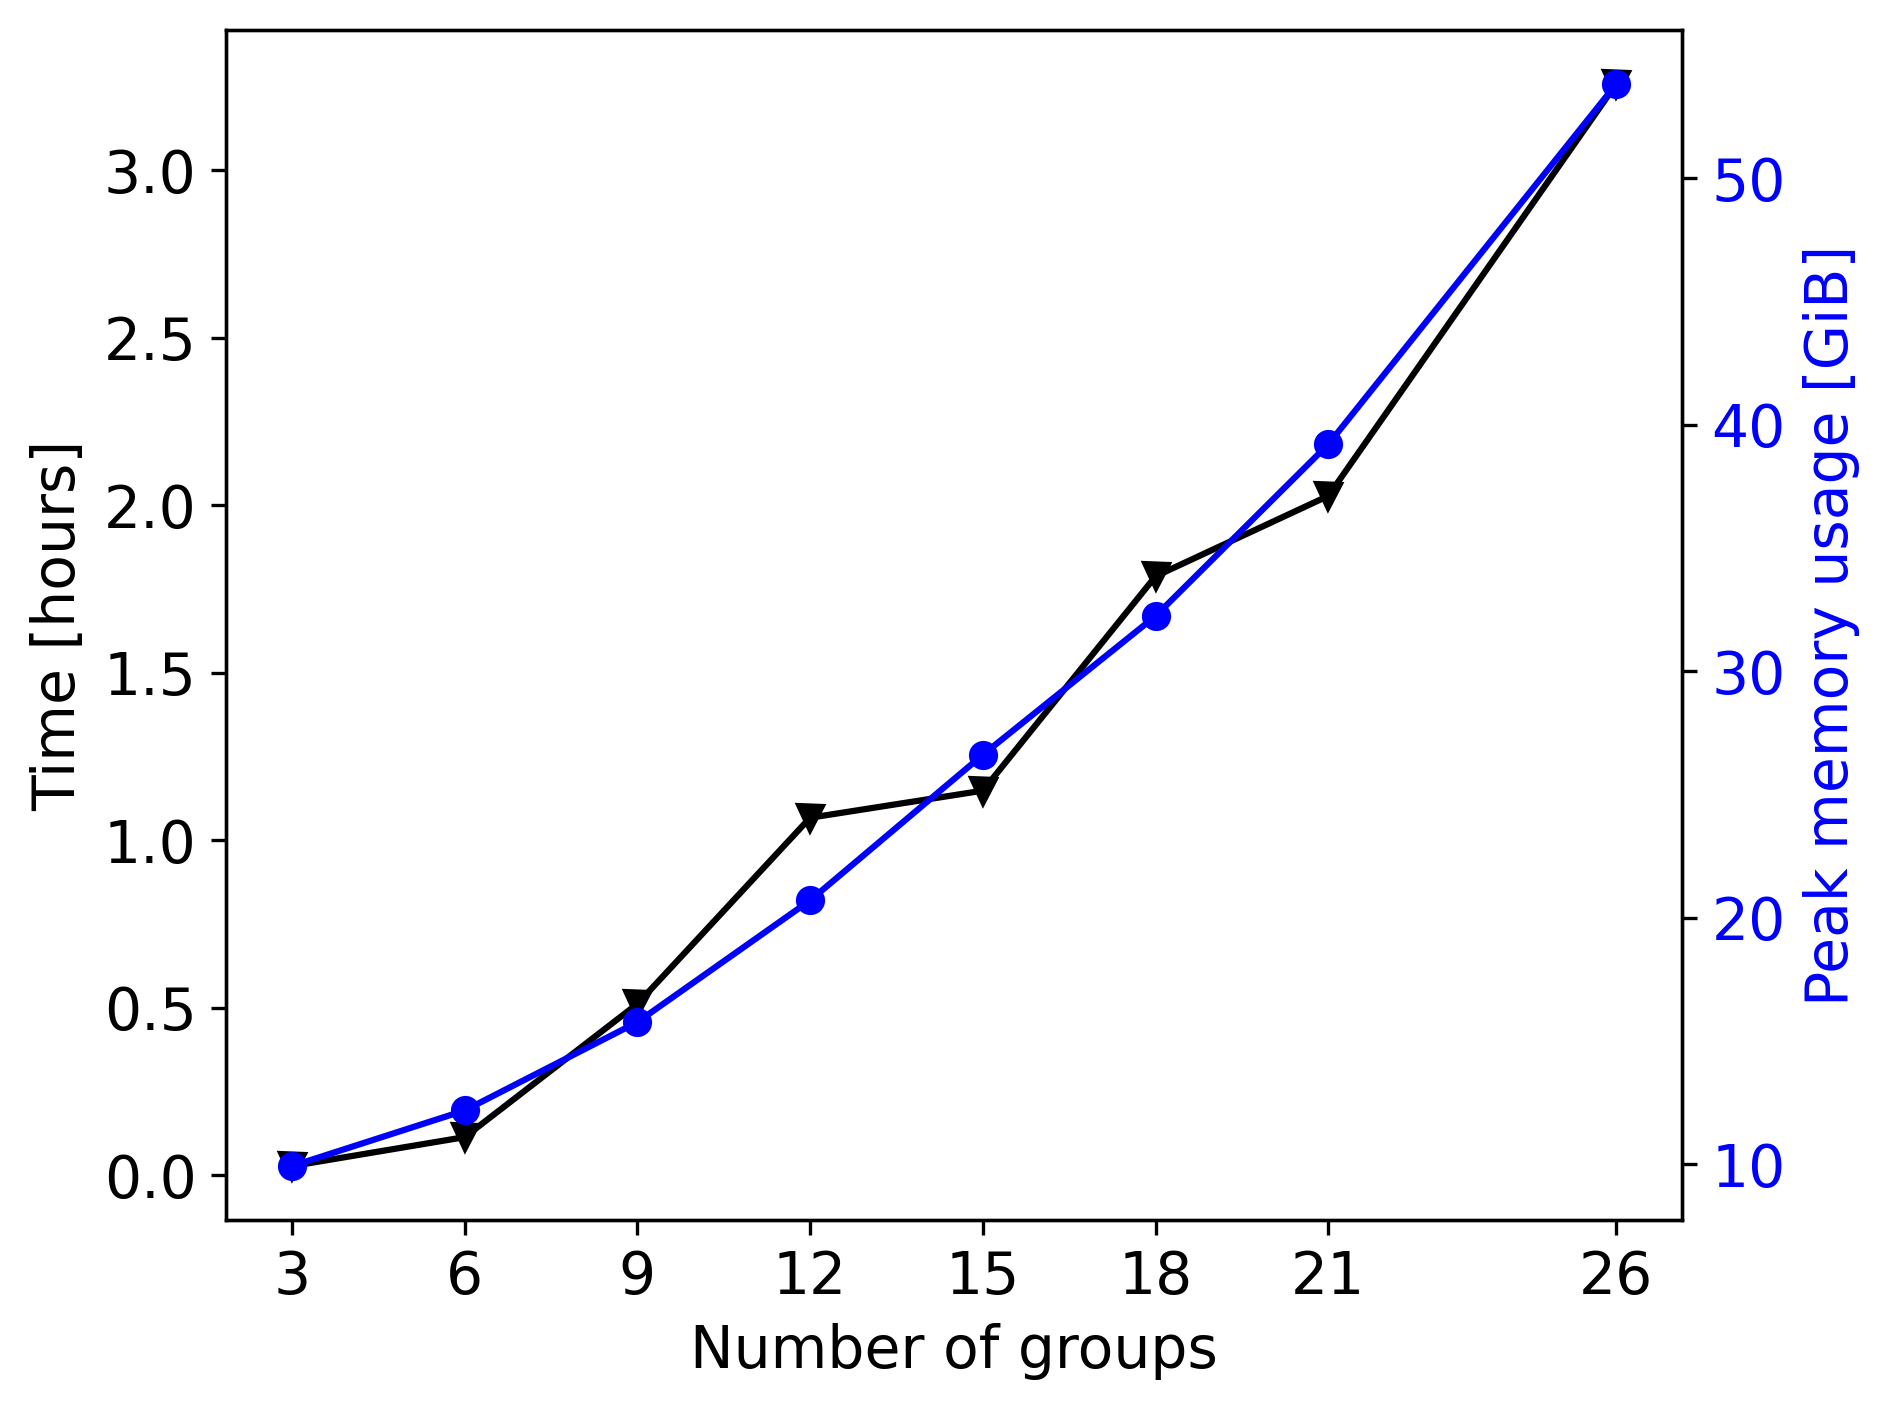
\includegraphics[width=0.45\textwidth]{figures-neutronics/time-noLBP-600}
    }
    \subfloat[Burnable poisons at 600 K.]{
        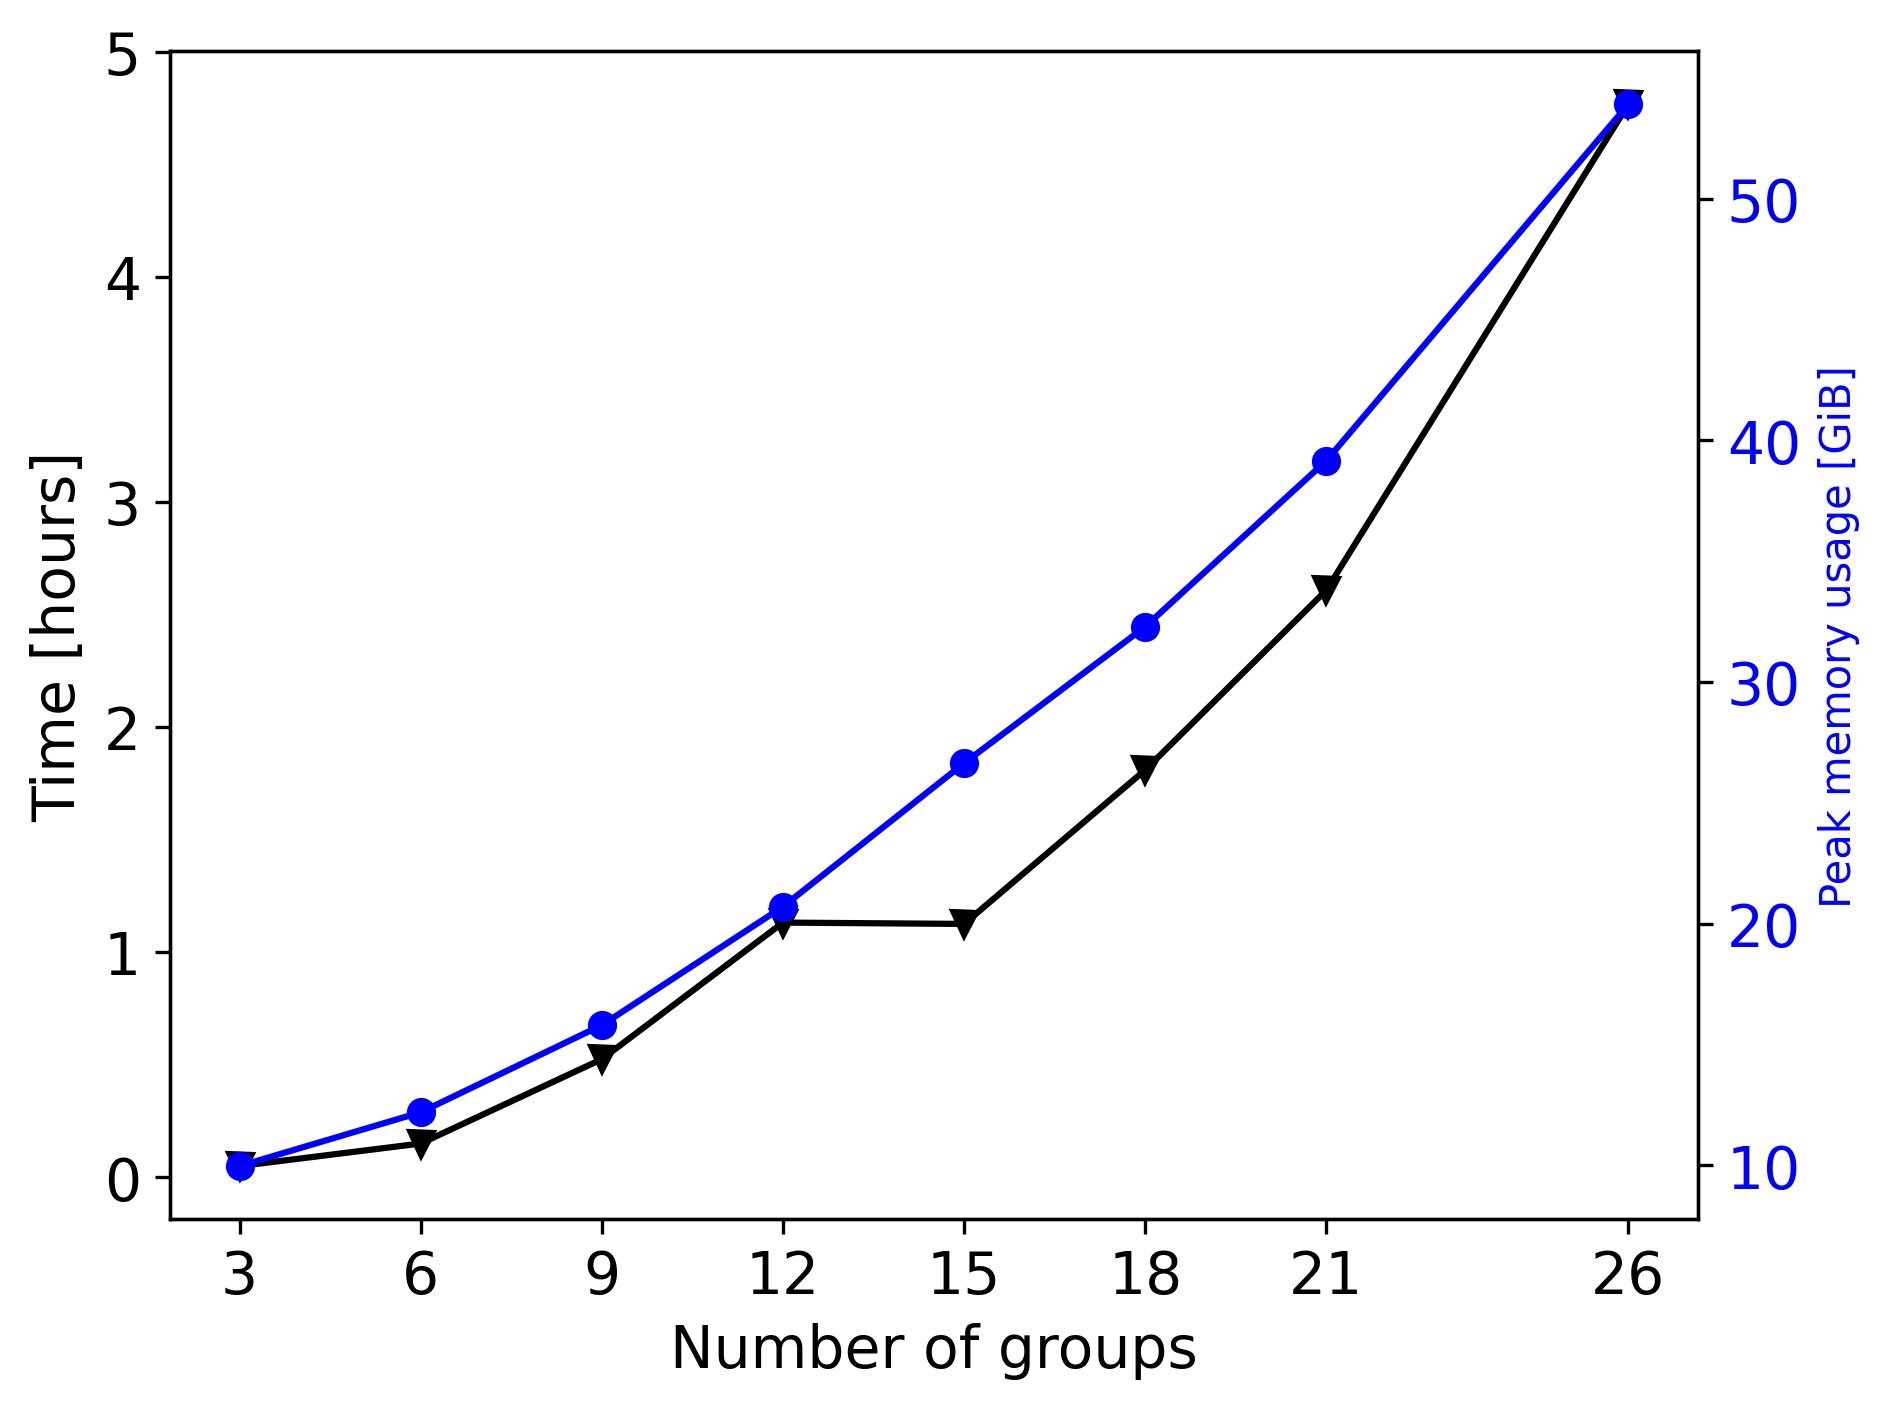
\includegraphics[width=0.45\textwidth]{figures-neutronics/time-LBP-600}
    }
	\hfill
	\caption{Computational time and memory requirements for different number of energy group structures.}
	\label{fig:assembly-time}
\end{figure}

The last study analyzed the impact of the energy group structure on the flux accuracy for a constant number of energy groups.
We chose 15 energy groups, as it yields a good overall accuracy and a practical computational expense.
Table \ref{tab:energygroups} defines the various energy group structures.
Table \ref{tab:accuracy15} exhibits the $L_2$-norm of the relative error for the various energy group structures.
Some energy group structures yield better results for some cases while giving worse results for others.
For example, the $15d$ structure gives better results at 600K with burnable poisons than without them.
To choose the best performing structure, equation \ref{eq:weighted-ave} calculated a weighted average for the different groups
\begin{align}
  & W_{ave} = w_{th} \Delta_{th} + w_{epi} \Delta_{epi} + w_{f} \Delta_{f} \label{eq:weighted-ave}
  \intertext{where}
  & W_{ave} = \mbox{weighted average } [-] \notag \\
  & w_{th} = \mbox{thermal flux weight } [-] \notag \\
  & w_{epi} = \mbox{epipthermal flux weight } [-] \notag \\
  & w_{f} = \mbox{fast flux weight } [-] \notag \\
  & \Delta_{th} = \mbox{L$_2$-norm relative difference of the thermal flux } [-] \notag \\
  & \Delta_{epi} = \mbox{L$_2$-norm relative difference of the epithermal flux } [-] \notag \\
  & \Delta_{f} = \mbox{L$_2$-norm relative difference of the fast flux } [-]. \notag
\end{align}

We arbitrarily chose the weights to be 0.5, 0.3, and 0.2 for the thermal, epithermal, and fast fluxes.
For this averaging scheme, the energy group structure $15d$ is the best one.

\begin{table}[htbp!]
  \centering
  \caption{Axial flux relative difference $L_2$-norm for various energy group structures. Values expressed in percentages.}
  \begin{tabular}{@{}l|c|l| S[table-format=2.1] S[table-format=2.1] S[table-format=2.1] S[table-format=2.1] S[table-format=2.1] }
  \toprule
	Burnable poisons     & Temperature {[}K{]}   & Flux       & \multicolumn{1}{c@{}}{15a} & \multicolumn{1}{c@{}}{15b}  & \multicolumn{1}{c@{}}{15c}  & \multicolumn{1}{c@{}}{15d}  & \multicolumn{1}{c@{}}{15e}  \\
	\midrule
	\multirow{6}{*}{No}  & \multirow{3}{*}{600}  & Fast       & 7.9  & 8.0  & 8.2  & 8.1  & 9.1  \\
	                     &                       & Epithermal & 6.6  & 6.5  & 8.6  & 8.2  & 9.2  \\
	                     &                       & Thermal    & 8.8  & 8.5  & 10.6 & 10.7 & 12.9 \\ \cline{2-8}
	                     & \multirow{3}{*}{1200} & Fast       & 7.1  & 7.7  & 5.7  & 5.1  & 4.5  \\
	                     &                       & Epithermal & 3.3  & 3.9  & 6.2  & 5.1  & 3.4  \\
	                     &                       & Thermal    & 5.0  & 4.7  & 8.5  & 8.2  & 8.4  \\ \hline
	\multirow{6}{*}{Yes} & \multirow{3}{*}{600}  & Fast       & 24.0 & 24.8 & 2.6  & 2.3  & 3.7  \\
	                     &                       & Epithermal & 21.0 & 21.7 & 2.0  & 1.6  & 2.7  \\
	                     &                       & Thermal    & 18.1 & 18.8 & 5.2  & 5.5  & 5.7  \\ \cline{2-8}
	                     & \multirow{3}{*}{1200} & Fast       & 36.2 & 37.3 & 6.9  & 6.6  & 25.9 \\
	                     &                       & Epithermal & 33.2 & 34.2 & 6.9  & 6.5  & 25.1 \\
	                     &                       & Thermal    & 29.6 & 30.6 & 8.5  & 8.3  & 20.3 \\
	\midrule
	\multicolumn{2}{l}{Weighted average}         &            & 17.3 & 17.8 & 6.3  & 6.0  & 10.8 \\
	\bottomrule
  \end{tabular}
  \label{tab:accuracy15}
\end{table}


\subsection{Full-core}

This section compared the results from Serpent and Moltres simulations of a full-core model.
Figure \ref{fig:fullcoremodel} displays a $xy$-plane of the model, which includes the bottom and top reflectors.
Due to symmetry, Moltres model included only a $1/6^{th}$ of the reactor.
The first step in the calculation obtained the group constants using Serpent.
Tables \ref{tab:maincharac}, \ref{tab:element-characteristics}, and \ref{tab:compact} specify the model input parameters.
For simplicity, standard fuel assemblies compose all the fuel column.
The model considered a fresh core, and it did not include the fuel handling holes nor the bottom and top reflector coolant channels.
Based on the previous section analyses, we chose the energy group structure $15d$ in Table \ref{tab:energygroups}.
The material temperatures were 600K and 1200K, cases that represent the \gls{CZP} and the \gls{HFP} core states.
The Serpent simulations included 8$\times 10^5$ neutrons per cycle, 500 active cycles, and 100 inactive cycles.

% Geometries
\begin{figure}[htbp!]
	\centering
    \subfloat[Serpent model geometry.]{
        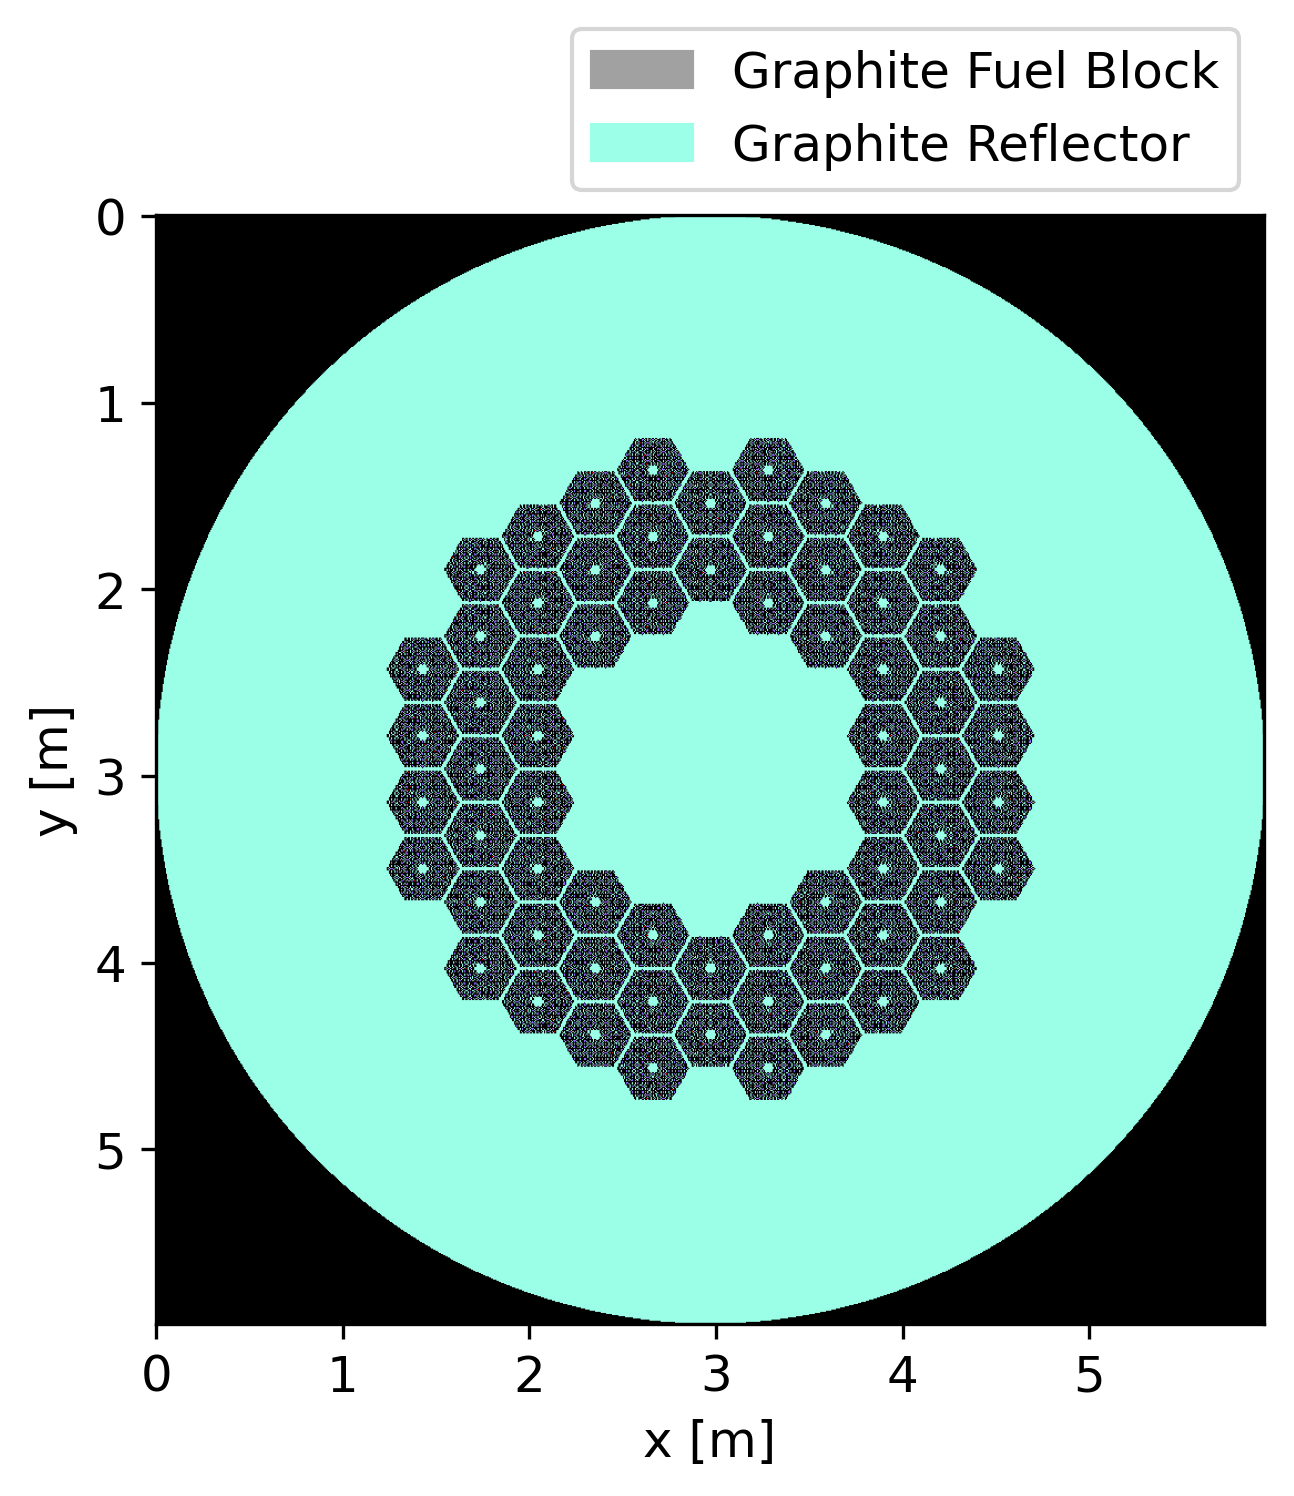
\includegraphics[width=0.39\textwidth]{figures-neutronics/oecd-fullcore}
    }
    \subfloat[Moltres model geometry.]{
        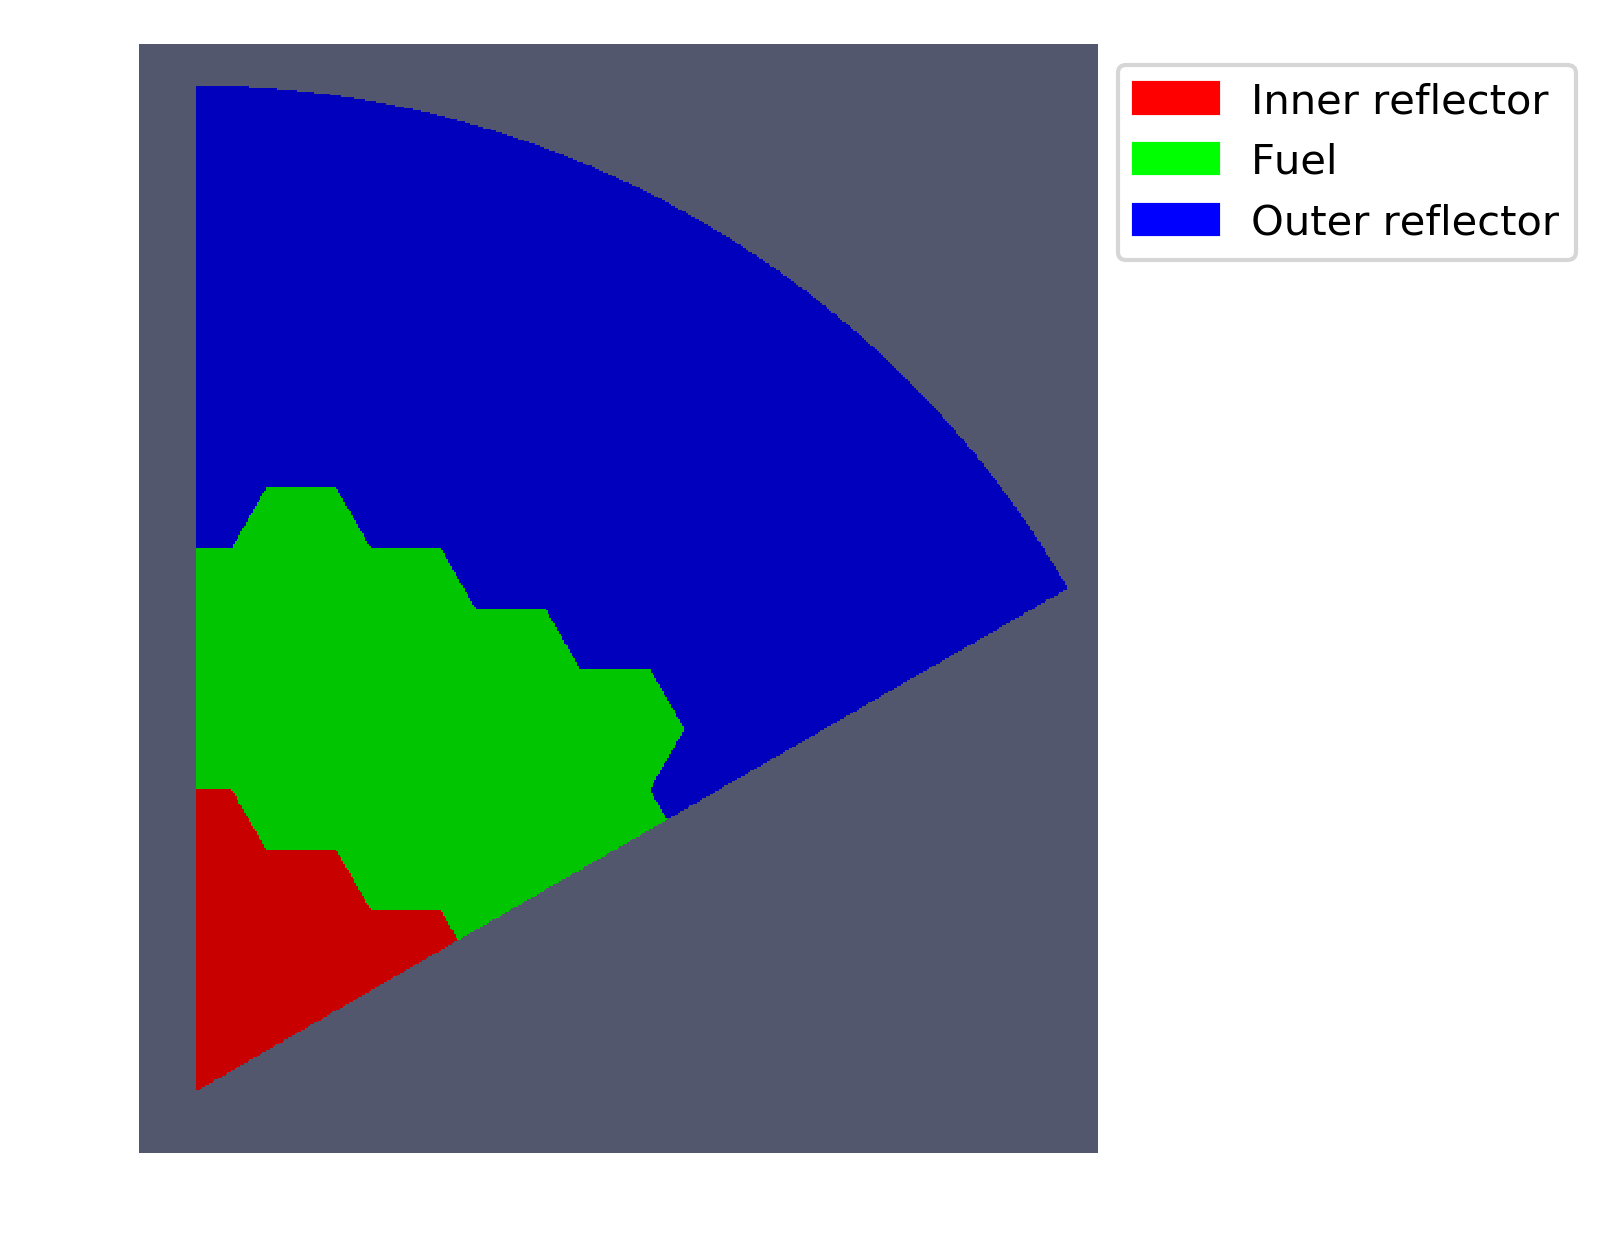
\includegraphics[width=0.49\textwidth]{figures-neutronics/3D-fullcore-60-homo-meshB2}
    }
	\hfill
  \caption{MHTGR-350 full-core model layout.}
	\label{fig:fullcoremodel}
\end{figure}

Moltres model geometry and mesh, which had 3.0 $\times 10^5$ elements and 1.60 $\times 1-^5$ nodes, using Gmsh.
The diffusion calculations had 1.60 $\times 10^5$ \glspl{DoF} per energy-group and a total of 2.4 $\times 10^6$ DoFs.
The Moltres input files set an eigenvalue and a flux convergence tolerance of 1$\times$10$^{-8}$.

% Keff
Between Serpent and Moltres, we compared the \gls{Keff}, the power distribution, and the flux shape and magnitude in different zones of the reactor.
Table \ref{tab:full-keff} exhibits the \gls{Keff} from Serpent and Moltres.
The differences between the eigenvalues calculated by Moltres and Serpent are smaller than 300 pcm.

\begin{table}[htbp!]
  \centering
  \caption{Comparison between Serpent and Moltres-derived eigenvalues.}
  \begin{tabular}{cccc}
  \toprule
  Temperature [K] & Serpent			     & Moltres  & $\Delta \rho$ [pcm] 	\\
  \midrule
			 600  	    & 1.10869 $\pm$ 0.00006  & 1.11150	 &	228		\\
			1200 	      & 1.06138 $\pm$ 0.00006  & 1.06468	 &	292   \\
  \bottomrule
  \end{tabular}
  \label{tab:full-keff}
\end{table}

% Power distribution
Figures \ref{fig:fullcore-600-power} and \ref{fig:fullcore-1200-power} show Serpent and Moltres radial power distributions.
The following analysis applies to both temperatures.
Regarding the power distribution, the results are symmetric with respect to a 60$^{\circ}$ line.
This suggests that we could reduce the mesh size by almost half by considering only $1/12^{th}$ of the reactor.
Next, we observe that Moltres result exhibits a higher power density than Serpent in the inner and outer rings but a lower power density in the middle ring.
The largest difference occurs at 600K, shown Figure \ref{fig:fullcore-600-power}, in the inner ring and has a magnitude of 0.29 MW.

%Power distribution at 600K
\begin{figure}[htbp!]
	\centering
    \subfloat[Serpent radial power distribution.]{
        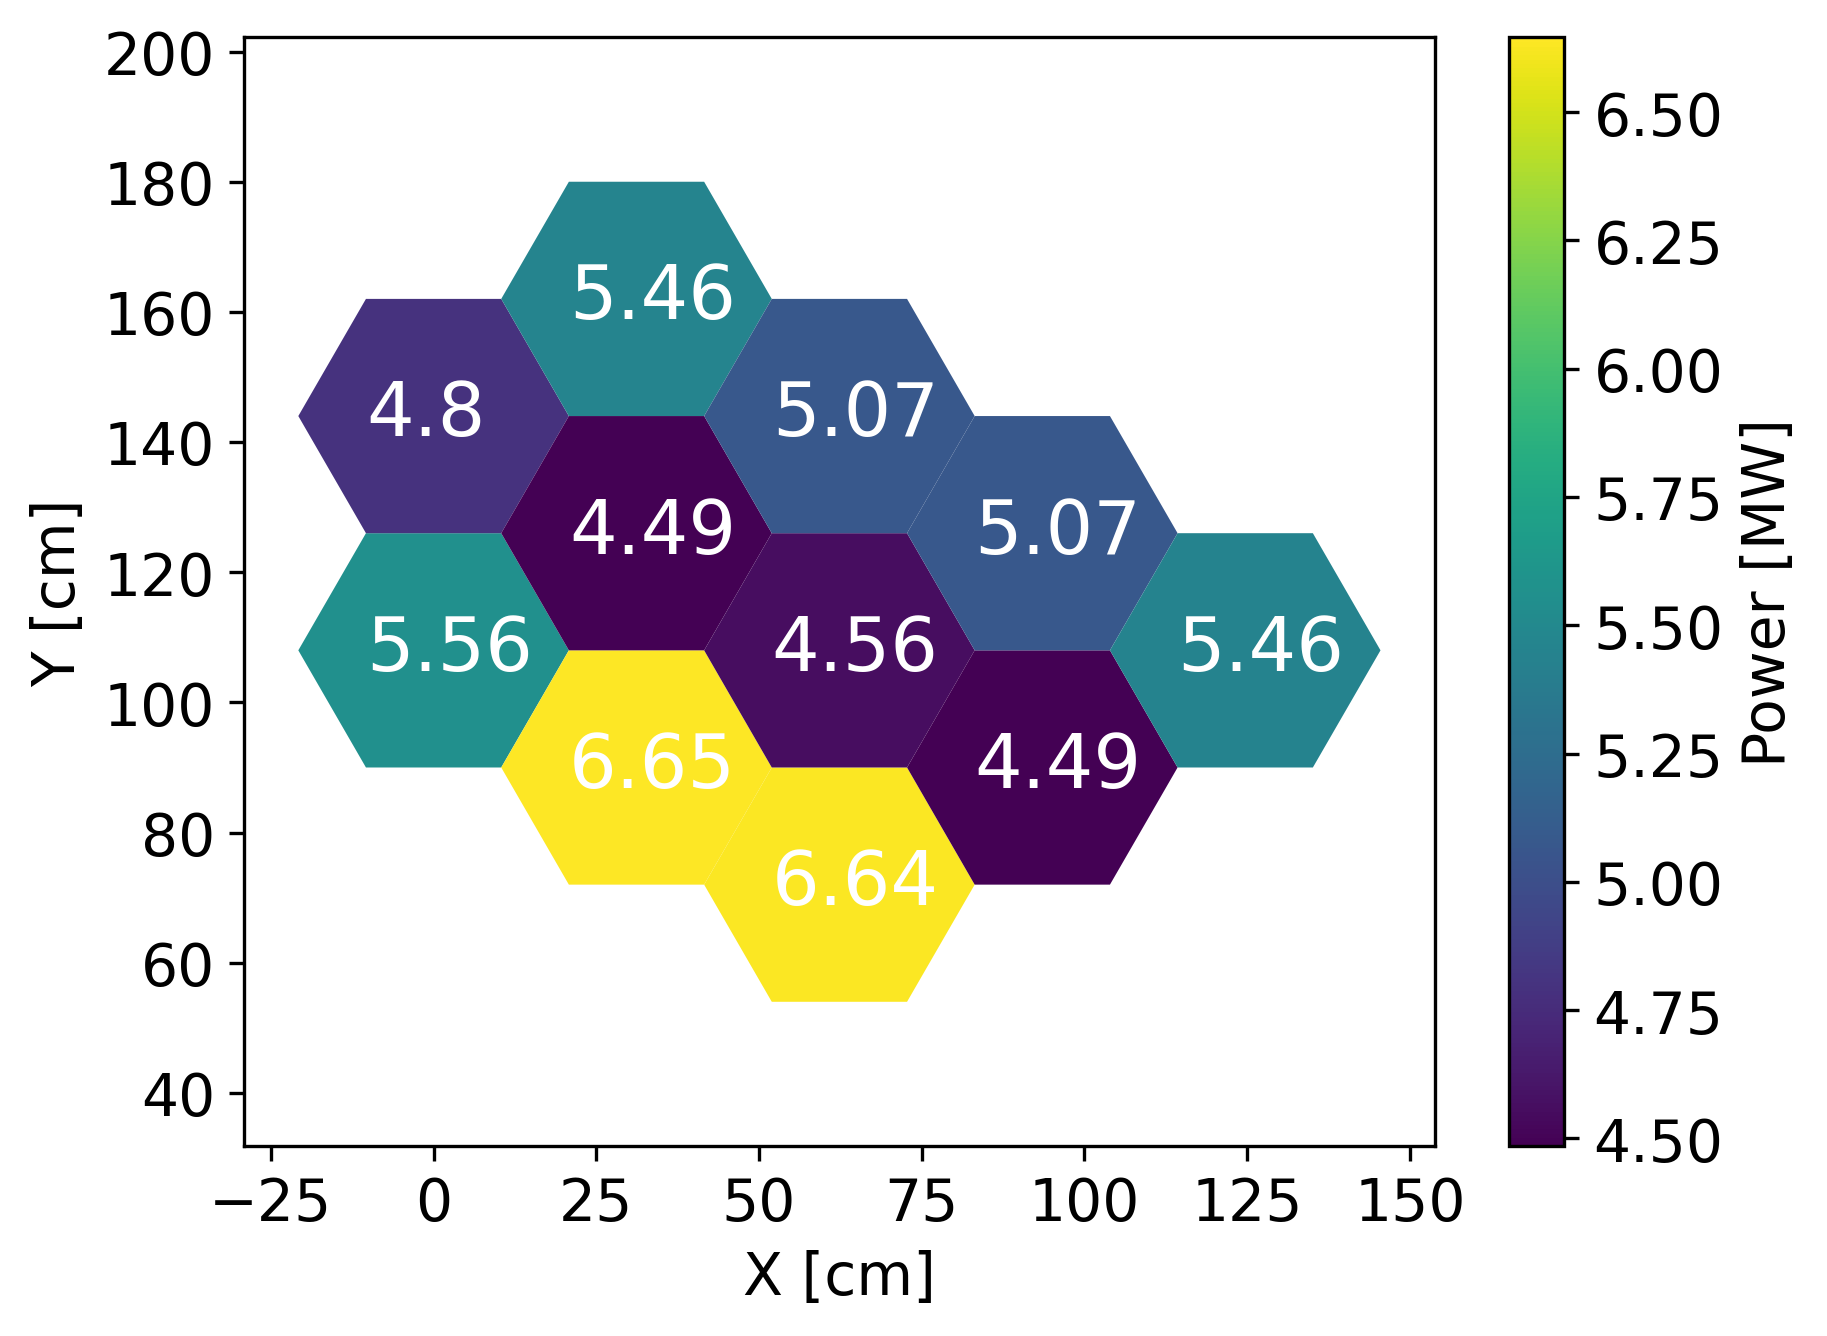
\includegraphics[width=0.45\textwidth]{figures-neutronics/serpent26G-600-power}
    }
    \subfloat[Moltres radial power distribution.]{
        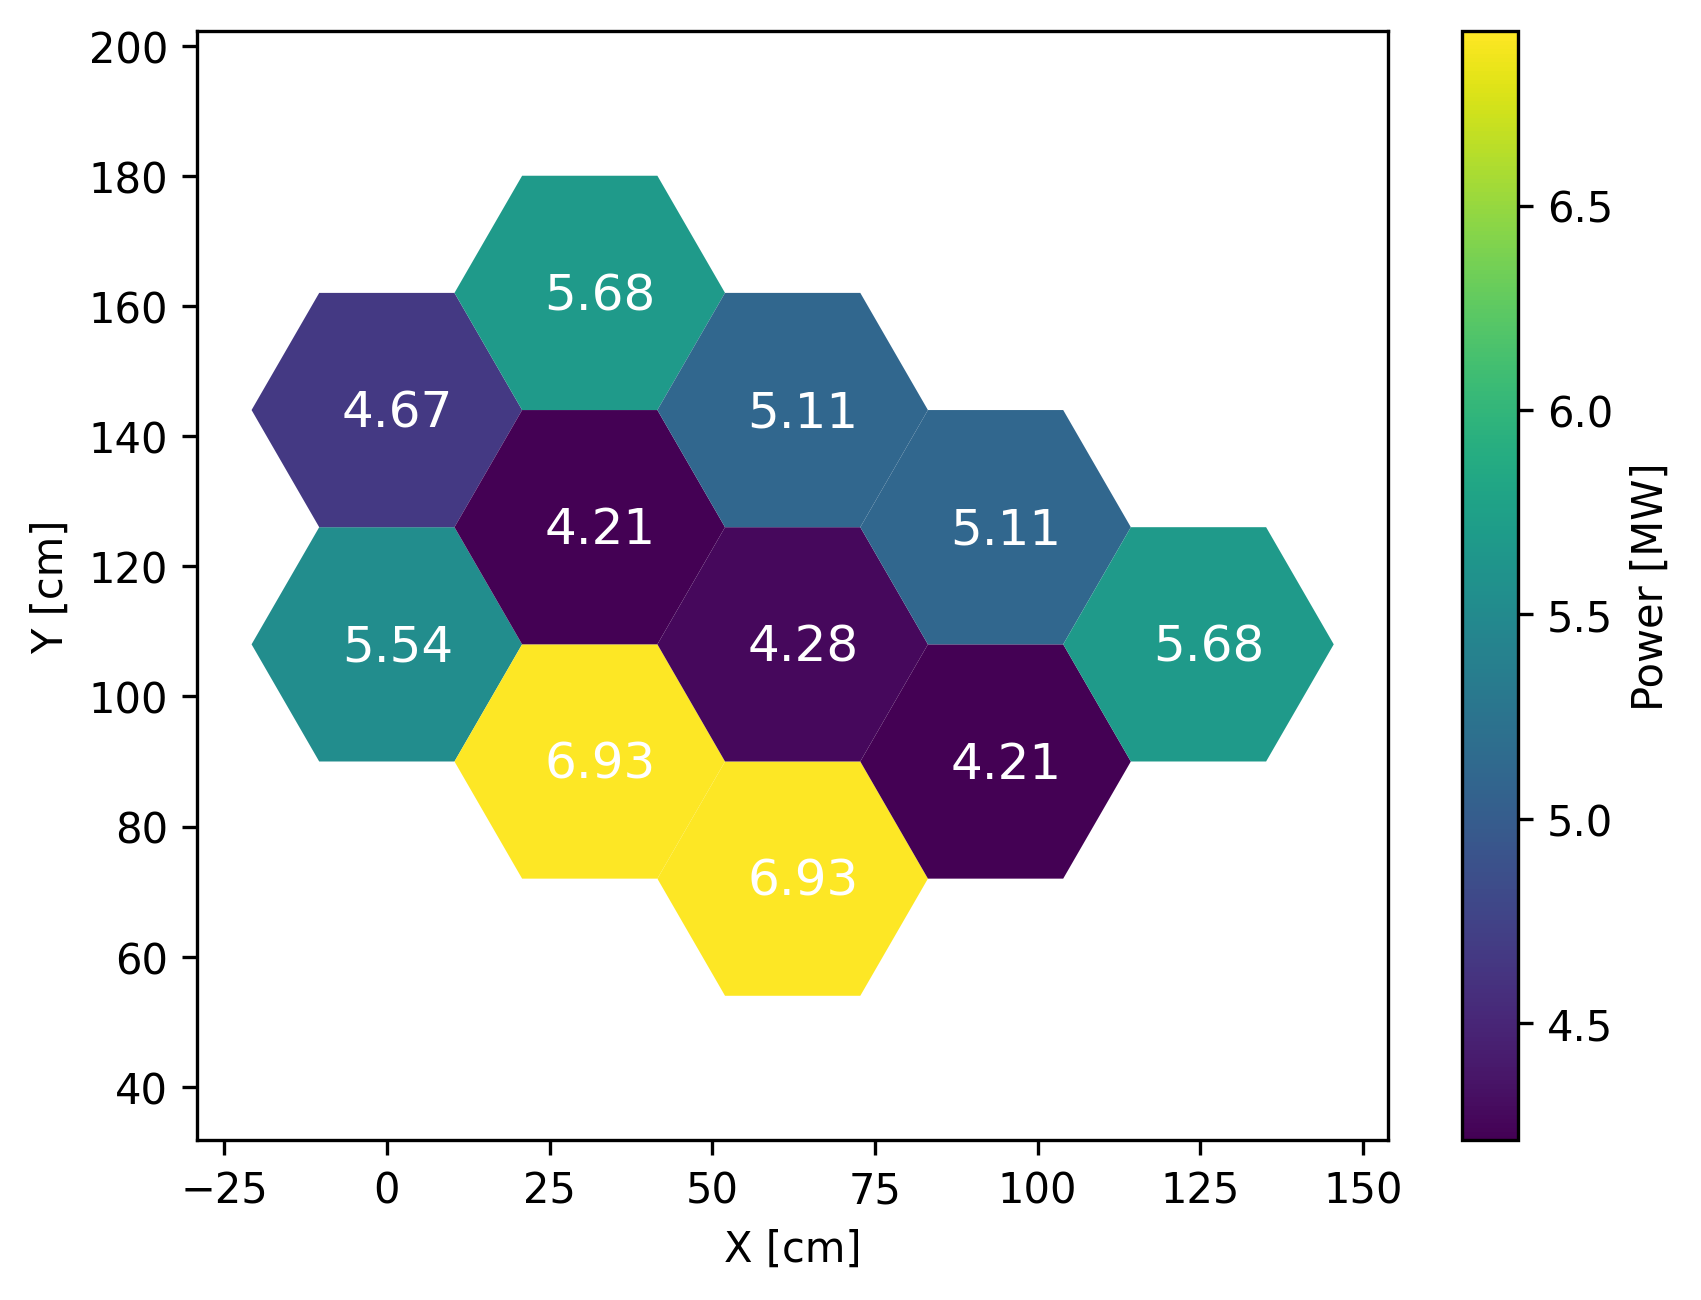
\includegraphics[width=0.45\textwidth]{figures-neutronics/3D-fullcore-600-15Gd-power}
    }
	\hfill
	\caption{Comparison of the MHTGR-350 radial power distribution at 600 K calculated by Serpent and Moltres.}
	\label{fig:fullcore-600-power}
\end{figure}

%Power distribution at 1200K
\begin{figure}[htbp!]
	\centering
    \subfloat[Serpent radial power distribution.]{
        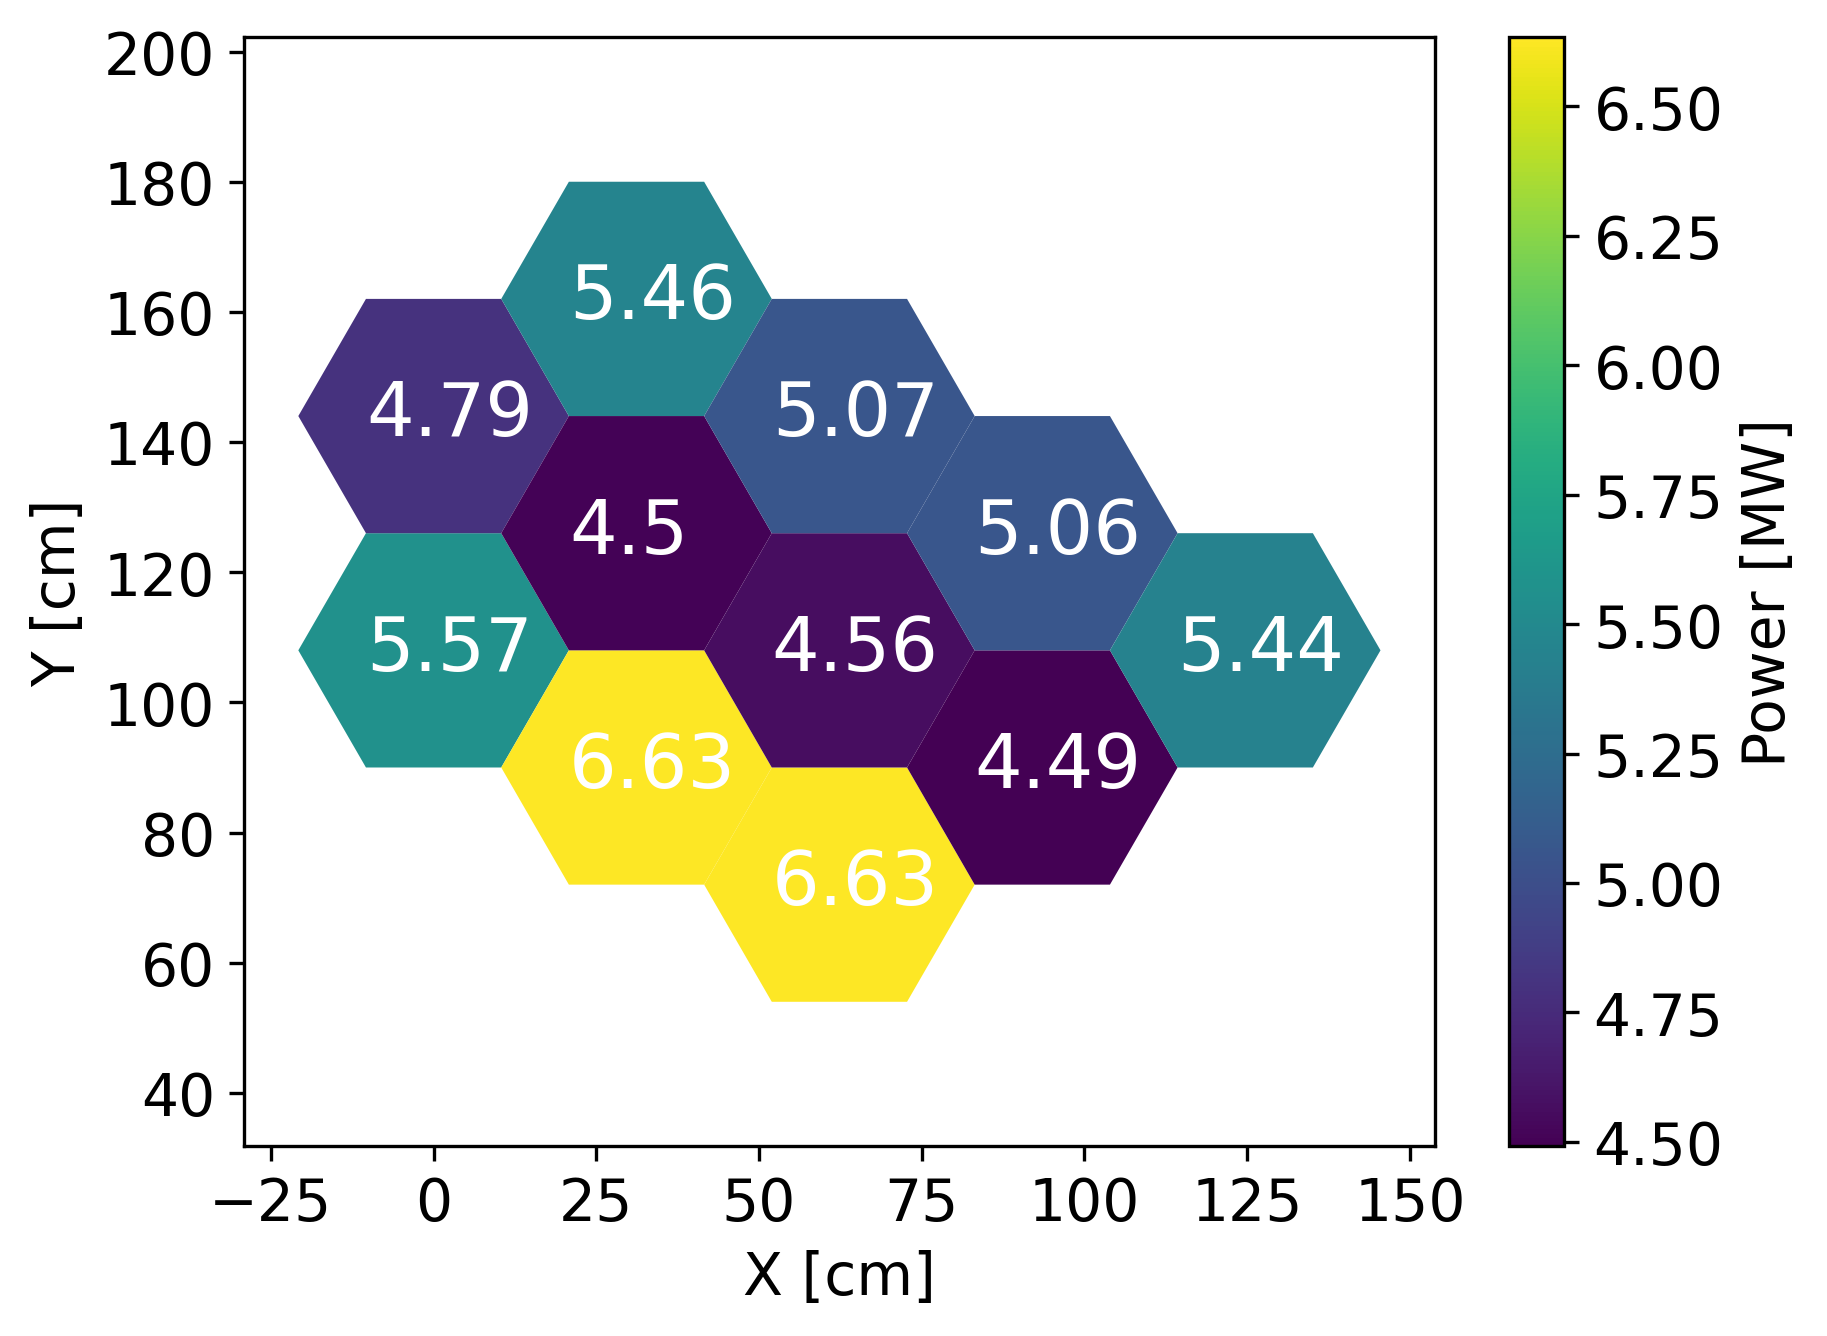
\includegraphics[width=0.45\textwidth]{figures-neutronics/serpent26G-1200-power}
    }
    \subfloat[Moltres radial power distribution.]{
        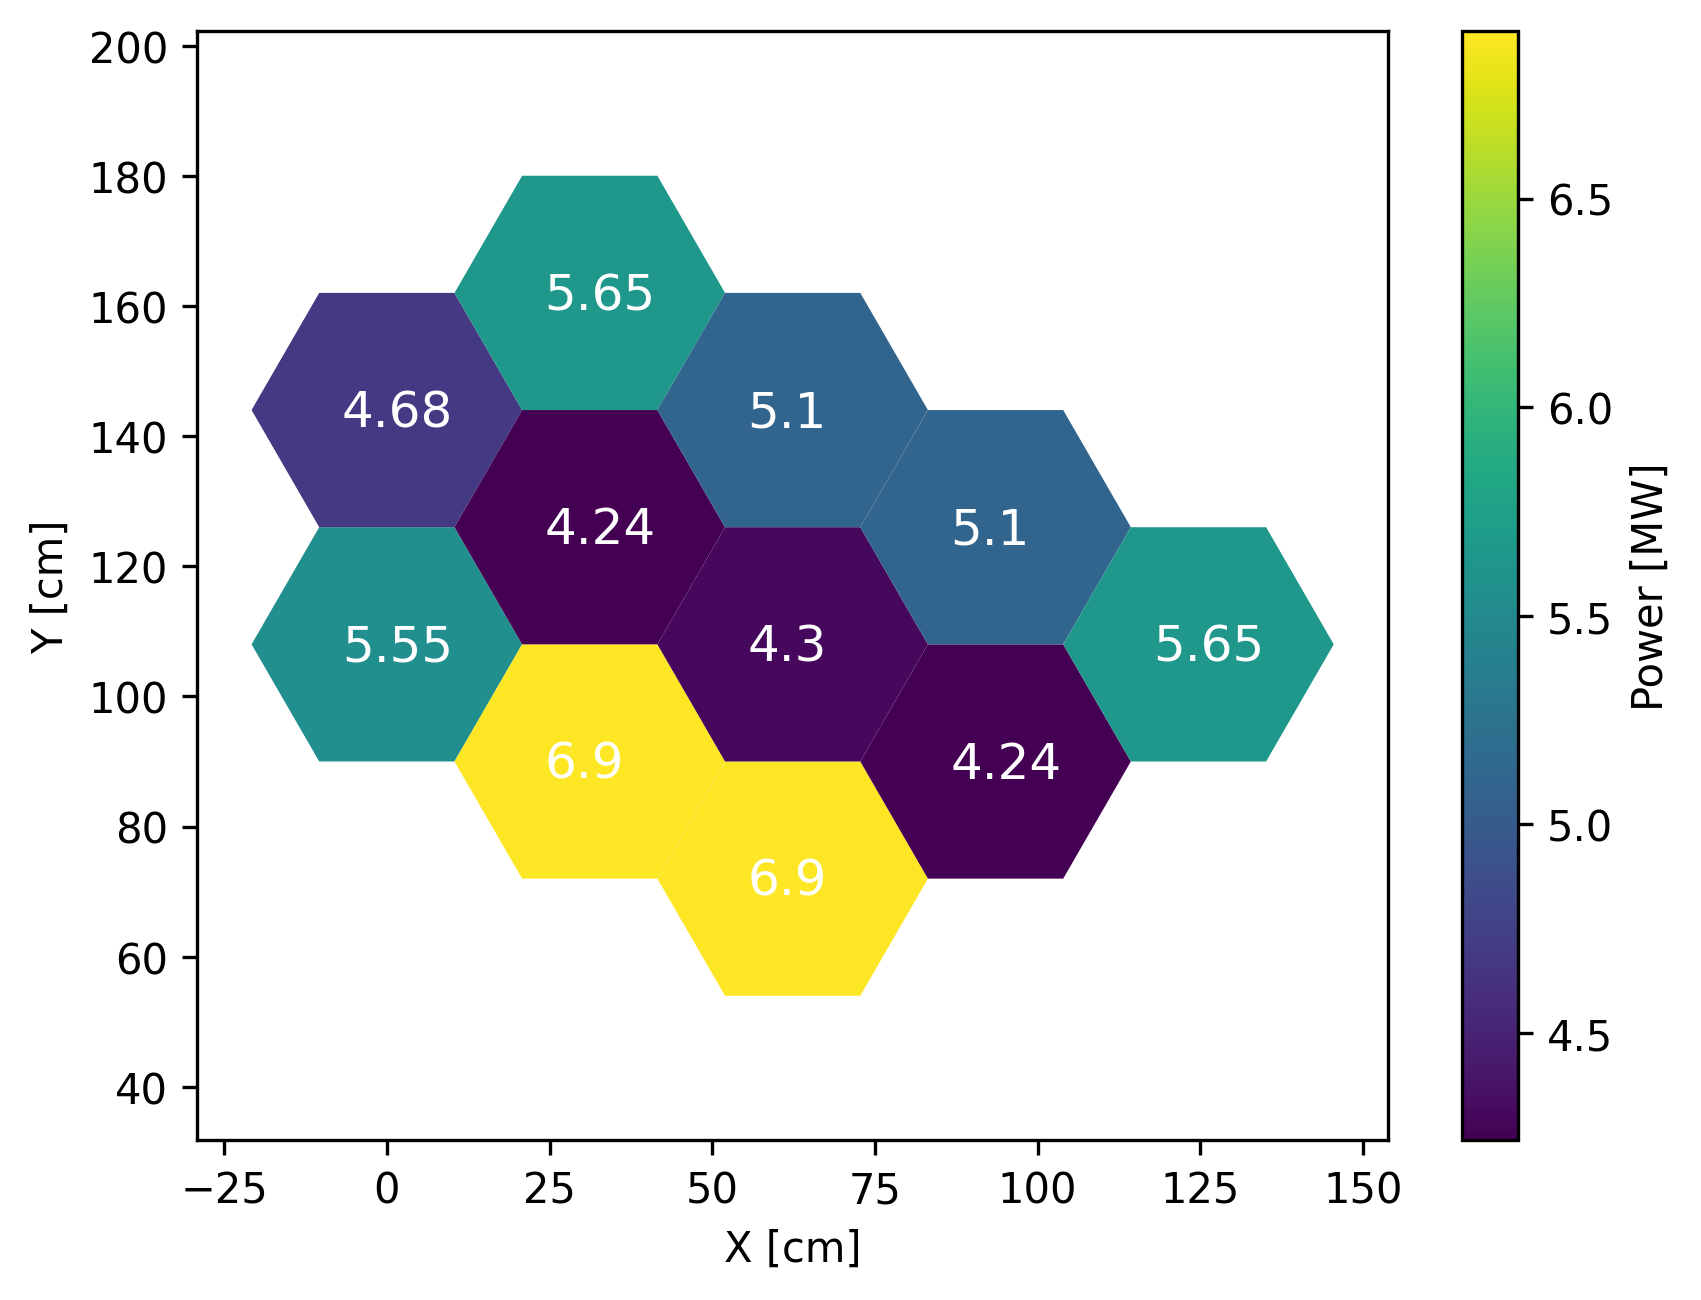
\includegraphics[width=0.45\textwidth]{figures-neutronics/3D-fullcore-1200-15Gc-power}
    }
	\hfill
	\caption{Comparison of the MHTGR-350 radial power distribution at 1200 K calculated by Serpent and Moltres.}
	\label{fig:fullcore-1200-power}
\end{figure}

% Fluxes
We placed axial and radial flux detectors in arbitrary regions of the reactor to compare the fluxes, Figure \ref{fig:fullcore-detectors} shows their locations.
Both the Serpent and Moltres radial detector's axial location was the middle of the active core's height.
Note that the flux in Serpent is an average over the fuel column's volume, while the flux in Moltres is the point-wise flux over the fuel column's centerline.
The Serpent radial detector's volume had a 2$^{\circ}$-angle and a fuel assembly's height.
Moltres ran the calculations for 15 energy groups and collapsed the results into three groups to facilitate the results' visualization.
Figures \ref{fig:fullcore-600-axial1} and \ref{fig:fullcore-600-radial1} show the axial and radial fluxes at 600K.
The axial flux shapes are similar, but Figure \ref{fig:fullcore-600-axial1} shows that the fast and epithermal axial fluxes in Moltres are larger, while the axial thermal flux is smaller.
The axial epithermal and thermal fluxes are closer in magnitude in the active core in Serpent's simulation.
In Figure \ref{fig:fullcore-600-radial1}, Serpent fluxes present some 'noise.'
A higher number of generations per cycle in Serpent simulations or using a detector with a larger volume would eliminate this.
Additionally, the radial flux in Serpent reveals the location of the burnable poisons in the fuel assemblies.
This diffusion simulation fails to capture such localized effects as the group constants are homogeneous in the fuel assembly.
The radial fast flux in Moltres is larger, while the radial epithermal and thermal fluxes have almost the same magnitudes.
Figures \ref{fig:fullcore-1200-axial1} and \ref{fig:fullcore-1200-radial1} display the fluxes at 1200K, which differ from the 600K case.
Still, we observe the same behavior for both axial and radial fluxes.
Overall, Moltres and Serpent fluxes are comparable in magnitude and shape.

%Detectors
\begin{figure}[htbp!]
	\centering
    \subfloat[Flux detectors in Serpent model.]{
        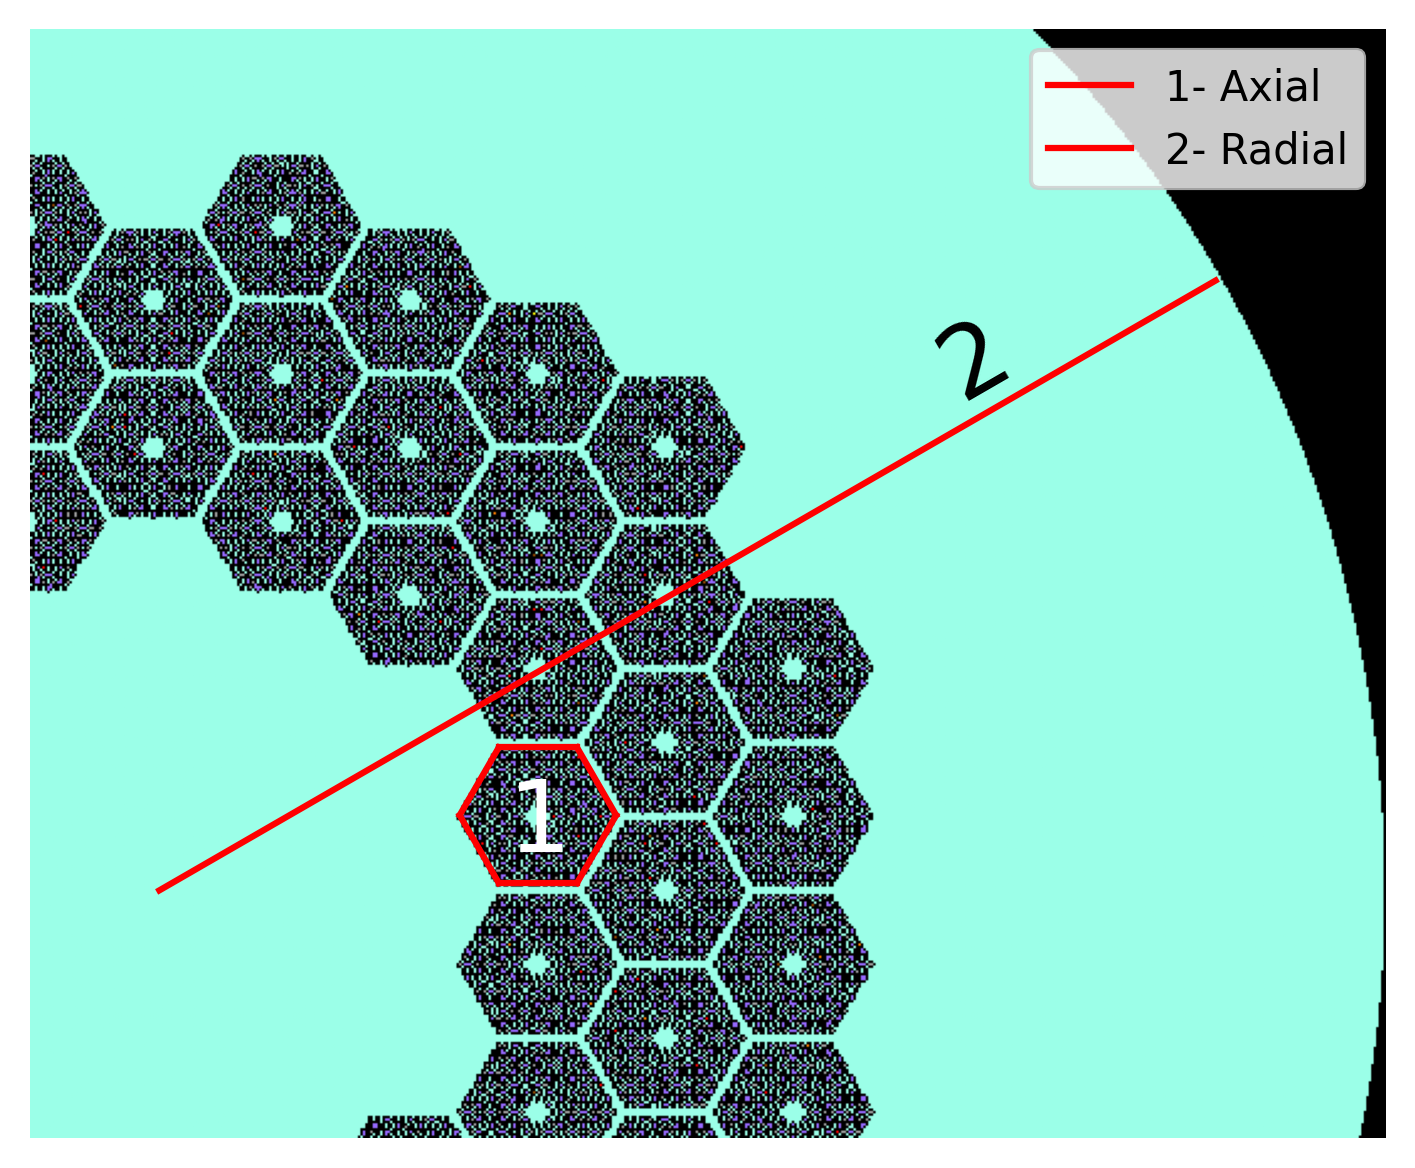
\includegraphics[width=0.52\textwidth]{figures-neutronics/oecd-fullcore-detectorsC}
    }
    \subfloat[Flux detectors in Moltres model.]{
        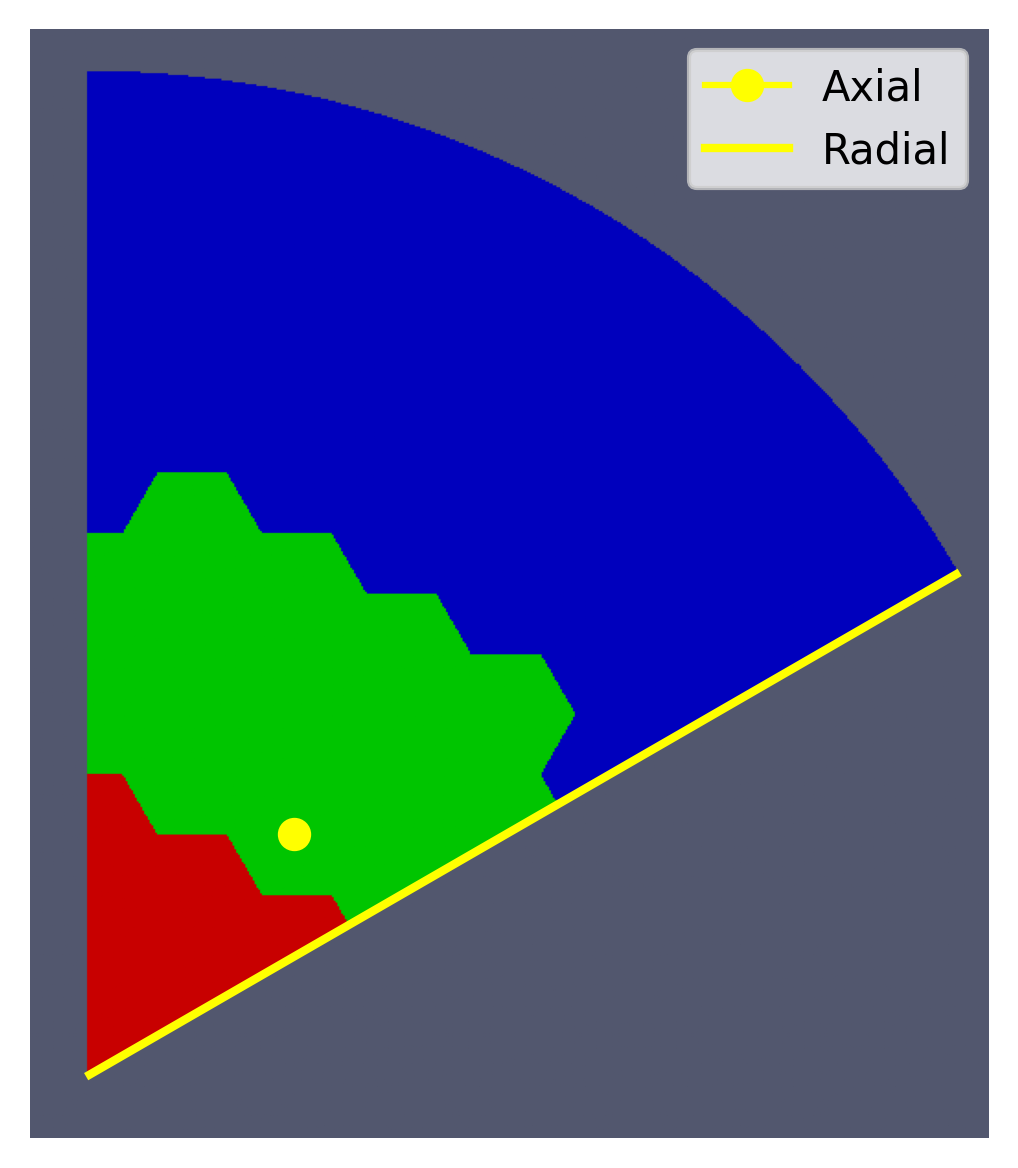
\includegraphics[width=0.37\textwidth]{figures-neutronics/3D-fullcore-60-detectors2}
    }
	\hfill
	\caption{Axial view of the flux detector locations.}
	\label{fig:fullcore-detectors}
\end{figure}

% Axial flux1 at 600K
\begin{figure}[htbp!]
	\centering
    \subfloat[Serpent axial detector flux.]{
        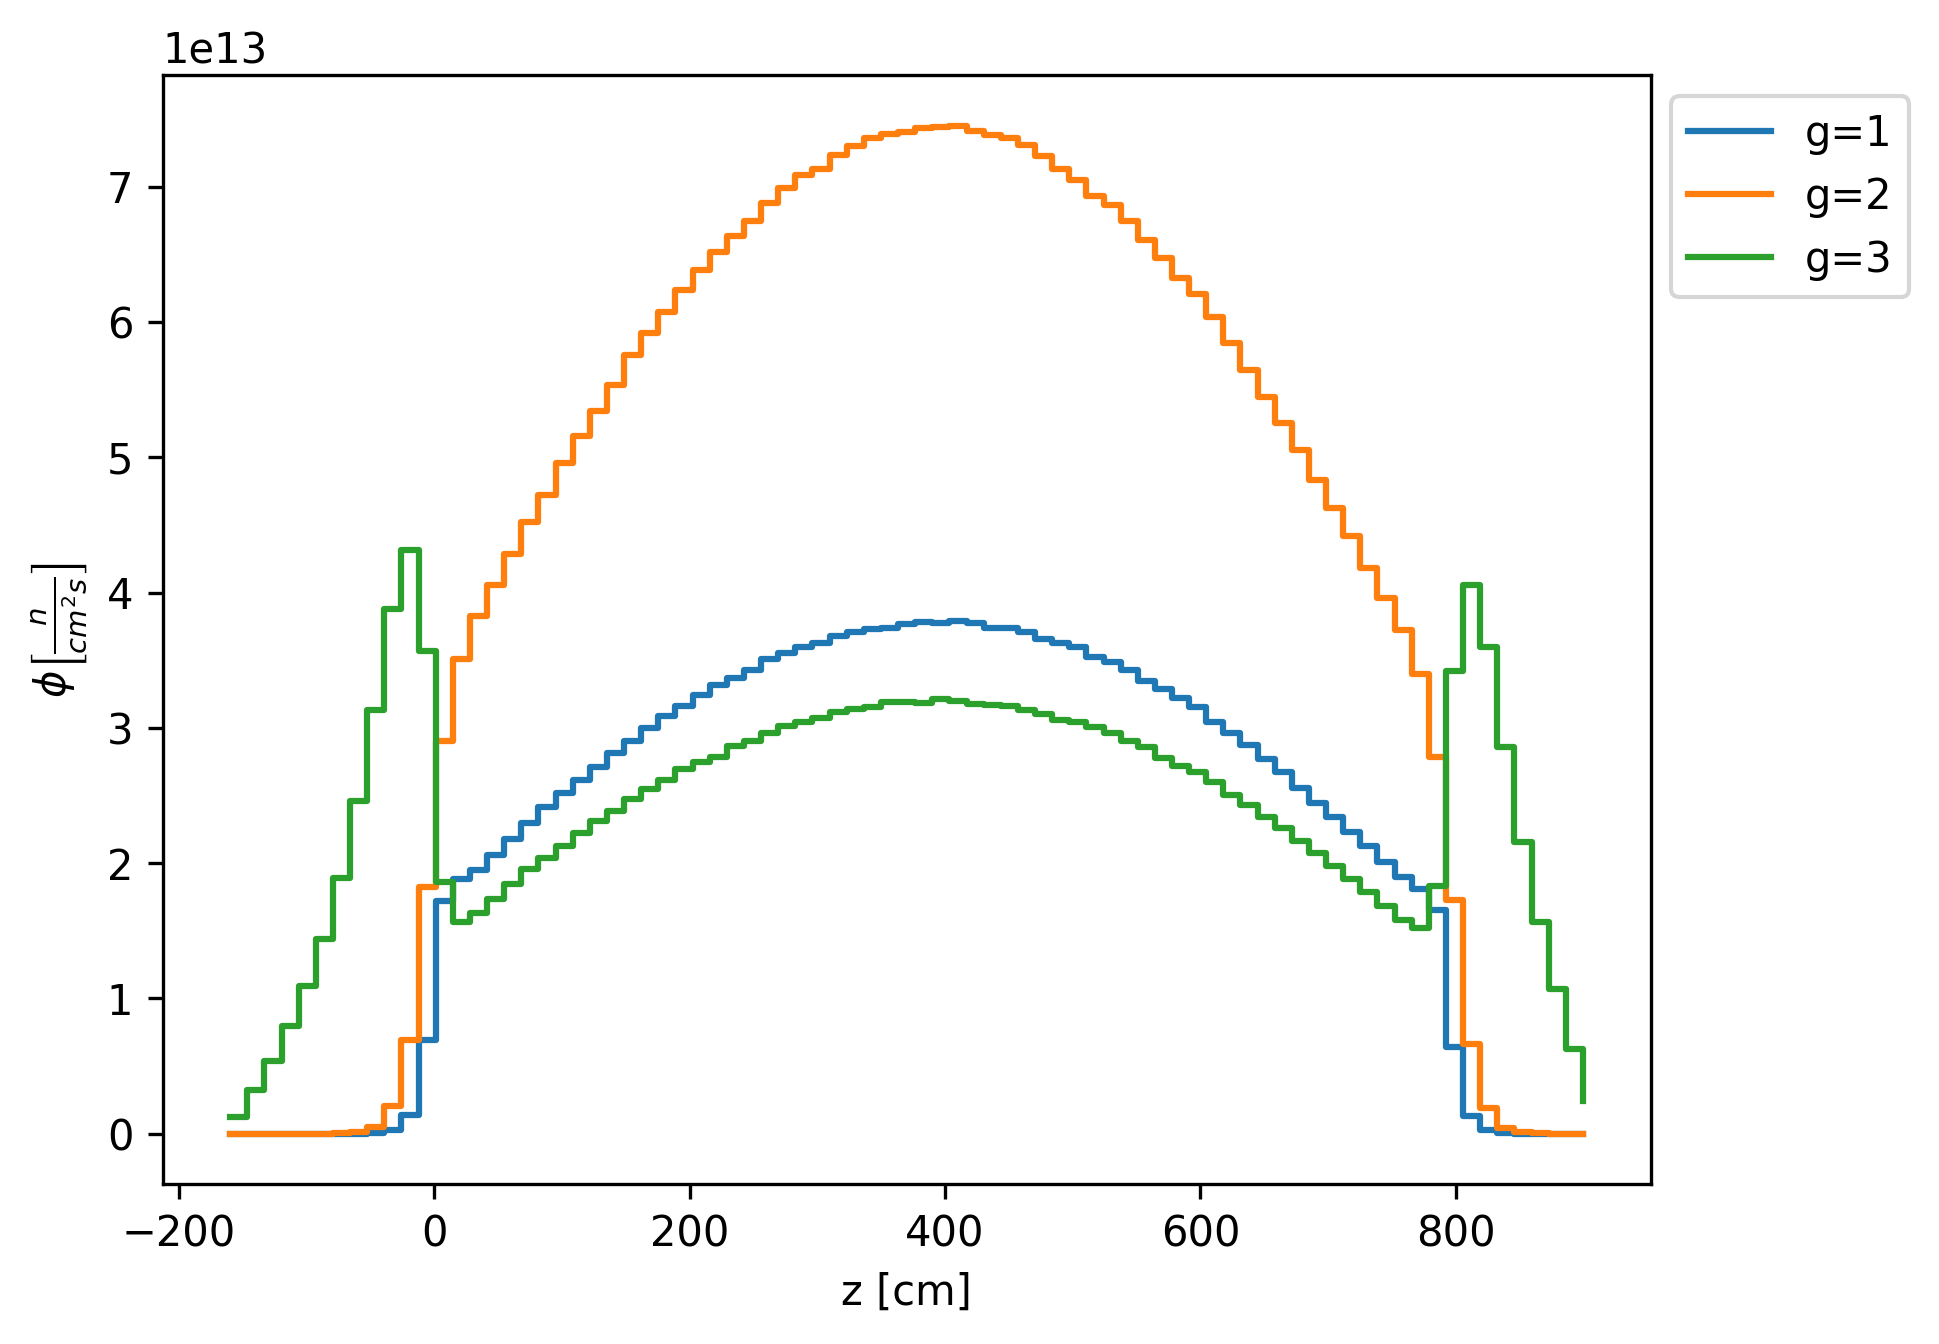
\includegraphics[width=0.45\textwidth]{figures-neutronics/serpent26G-600-collapse-Axial1}
    }
    \subfloat[Moltres axial detector flux.]{
        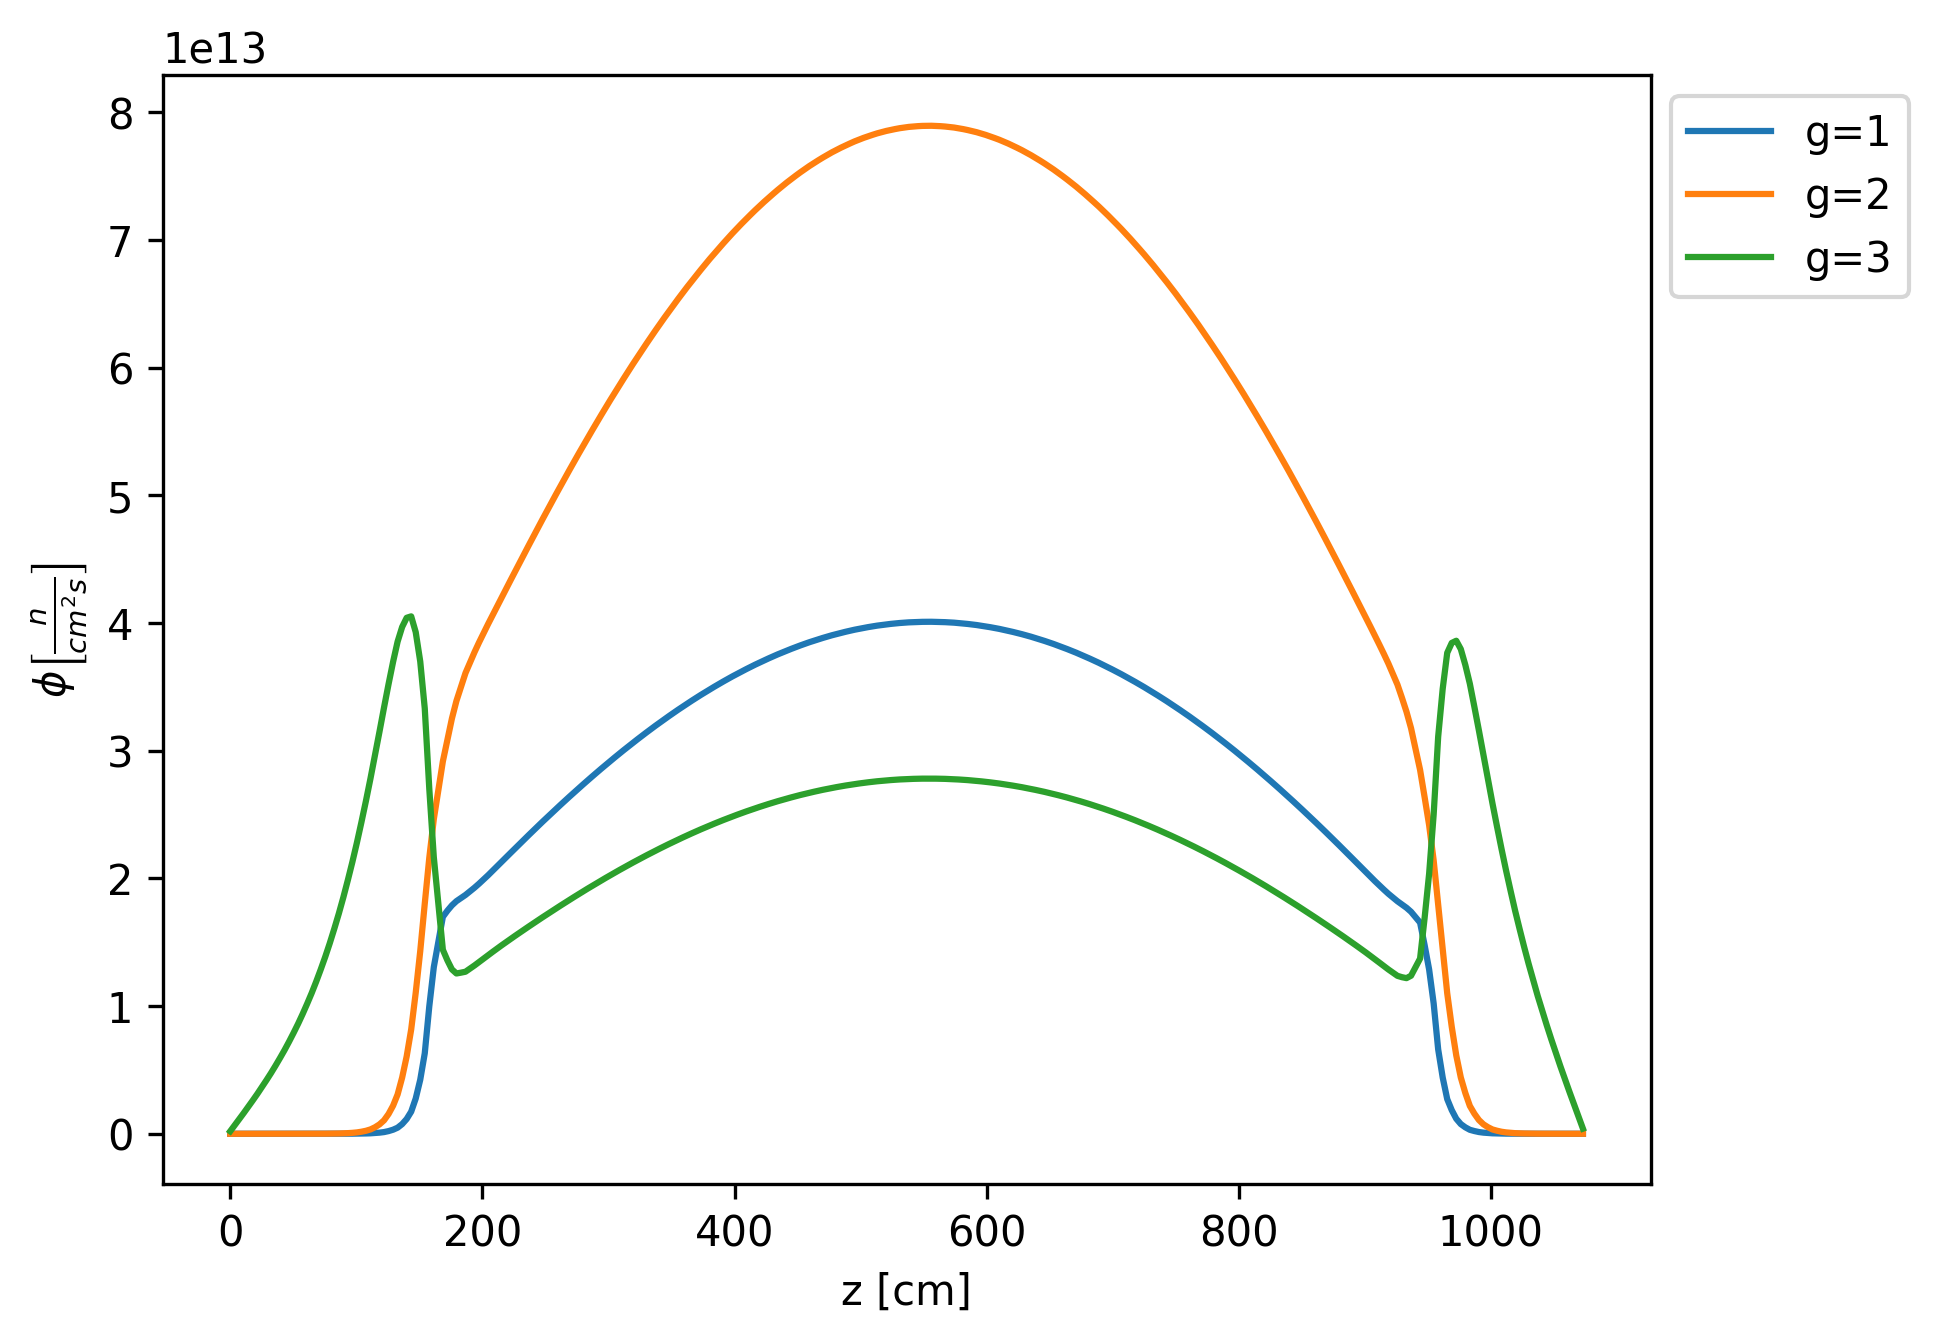
\includegraphics[width=0.45\textwidth]{figures-neutronics/3D-fullcore-600-15Gd-axial1}
    }
	\hfill
	\caption{Comparison of the axial detector flux calculated by Serpent and Moltres at 600 K.}
	\label{fig:fullcore-600-axial1}
\end{figure}

%Radial flux at 600 K
\begin{figure}[htbp!]
	\centering
    \subfloat[Serpent radial detector flux.]{
        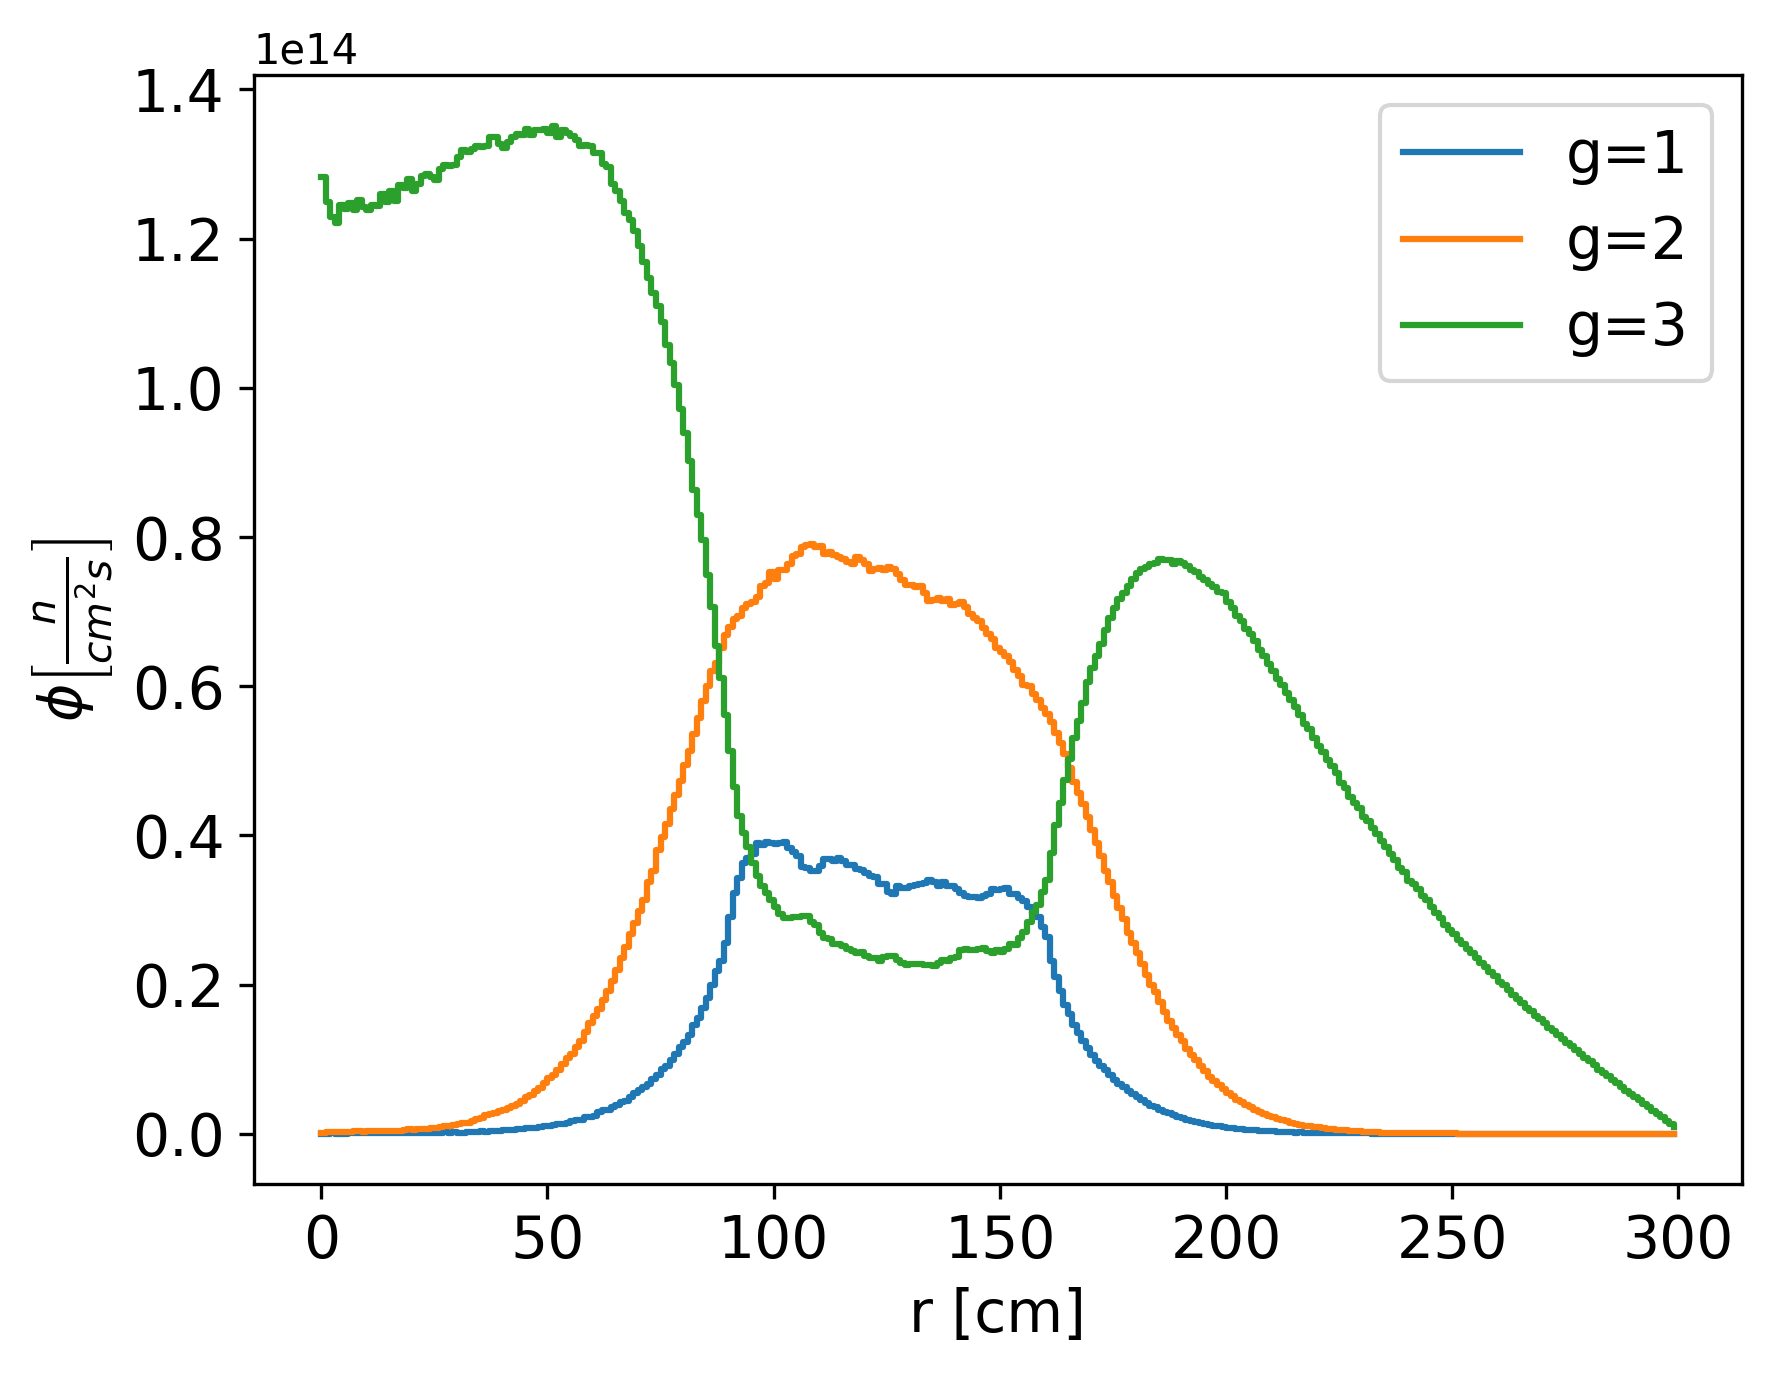
\includegraphics[width=0.45\textwidth]{figures-neutronics/serpent26G-600-collapse-Radial}
    }
    \subfloat[Moltres radial detector flux.]{
        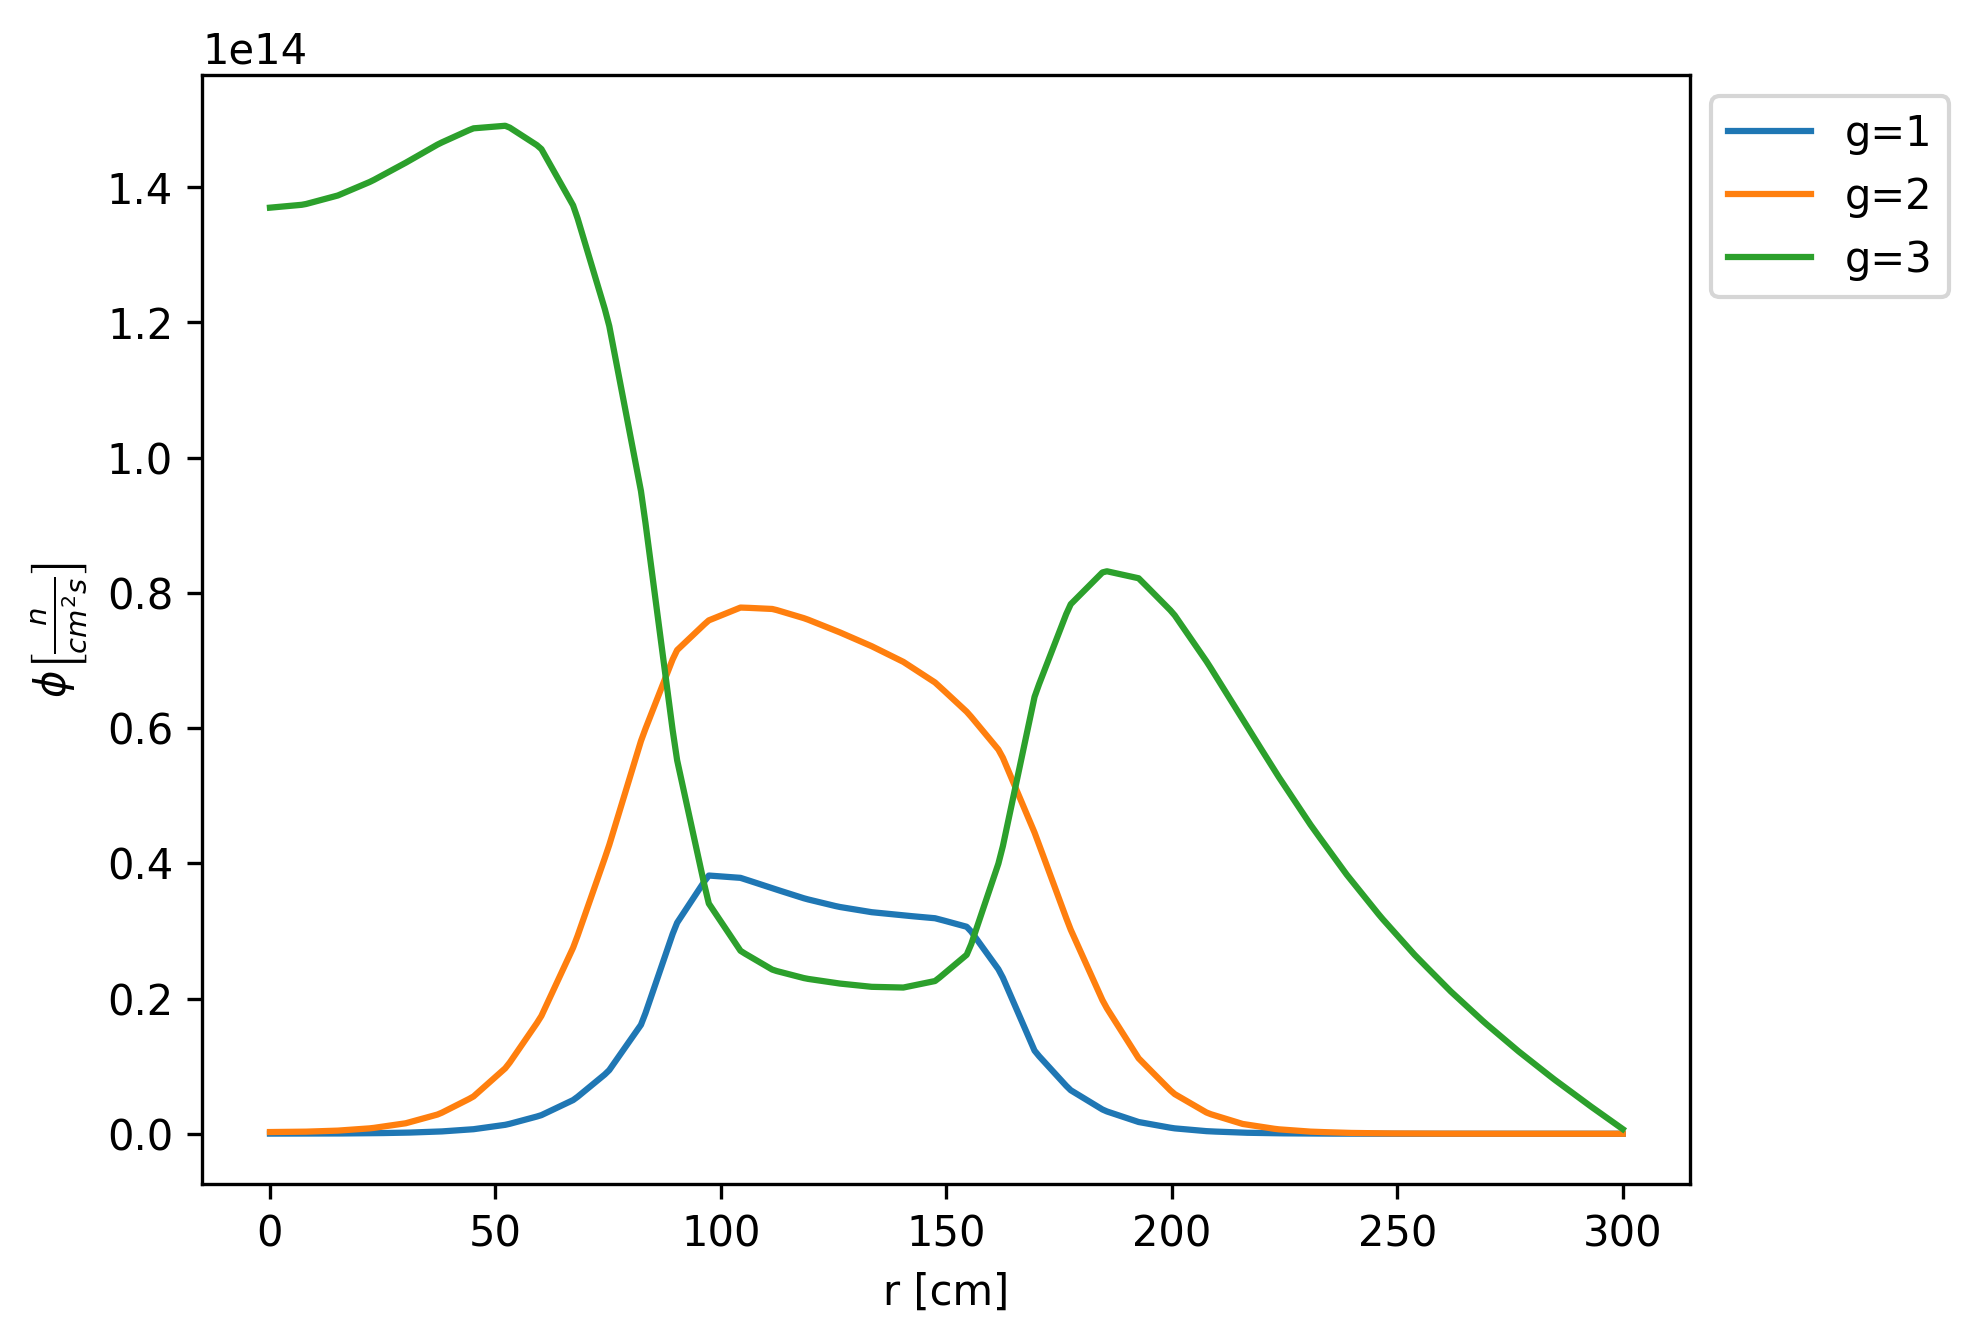
\includegraphics[width=0.45\textwidth]{figures-neutronics/3D-fullcore-600-15Gd-radial1}
    }
	\hfill
	\caption{Comparison of the radial detector flux calculated by Serpent and Moltres at 600 K.}
	\label{fig:fullcore-600-radial1}
\end{figure}

% Axial flux1 at 1200K
\begin{figure}[htbp!]
	\centering
    \subfloat[Serpent axial detector flux.]{
        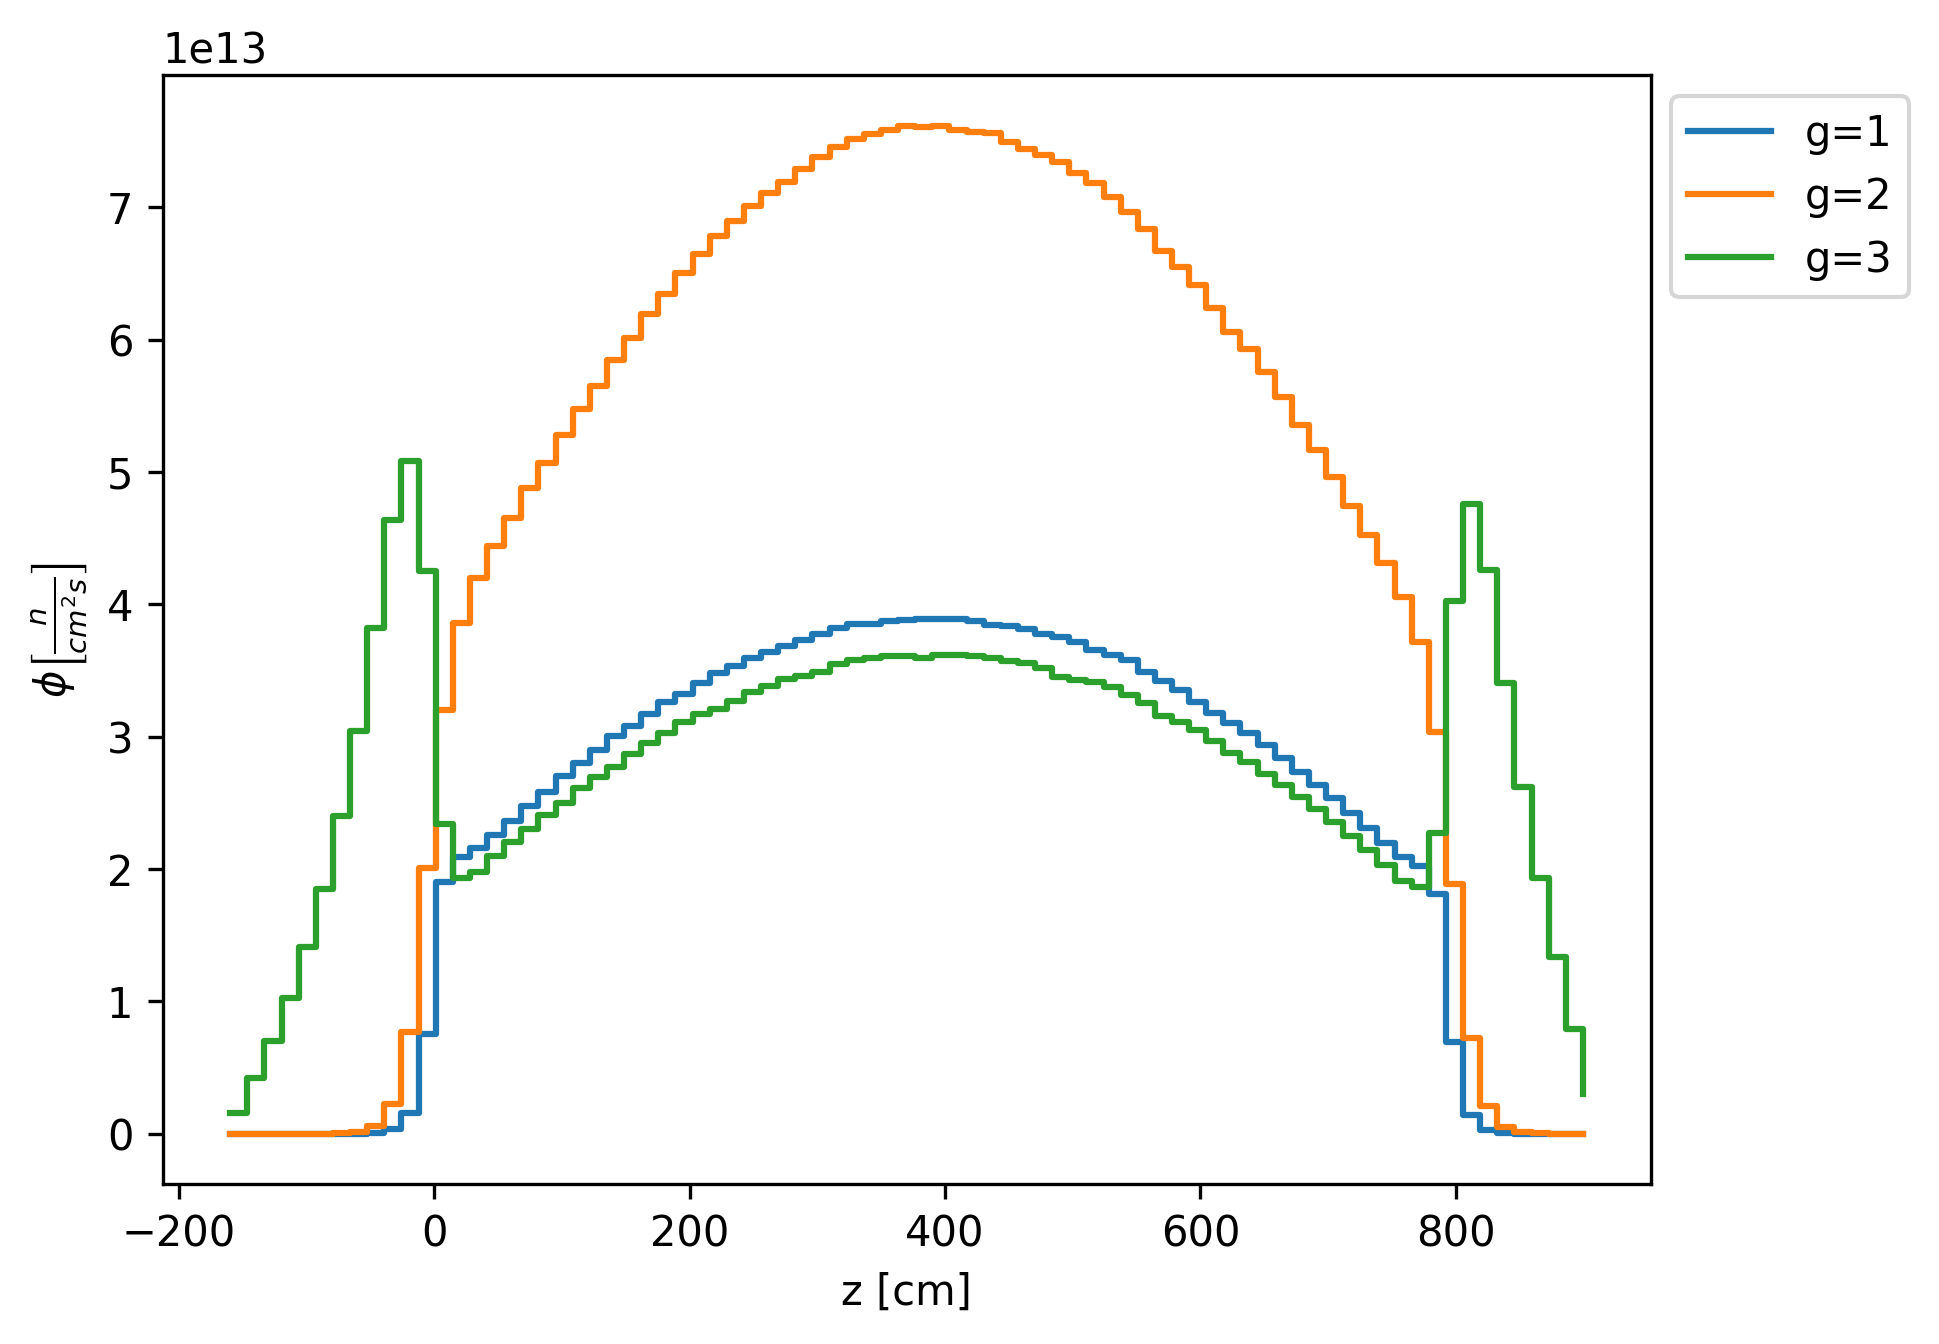
\includegraphics[width=0.45\textwidth]{figures-neutronics/serpent26G-1200-collapse-Axial1}
    }
    \subfloat[Moltres axial detector flux.]{
        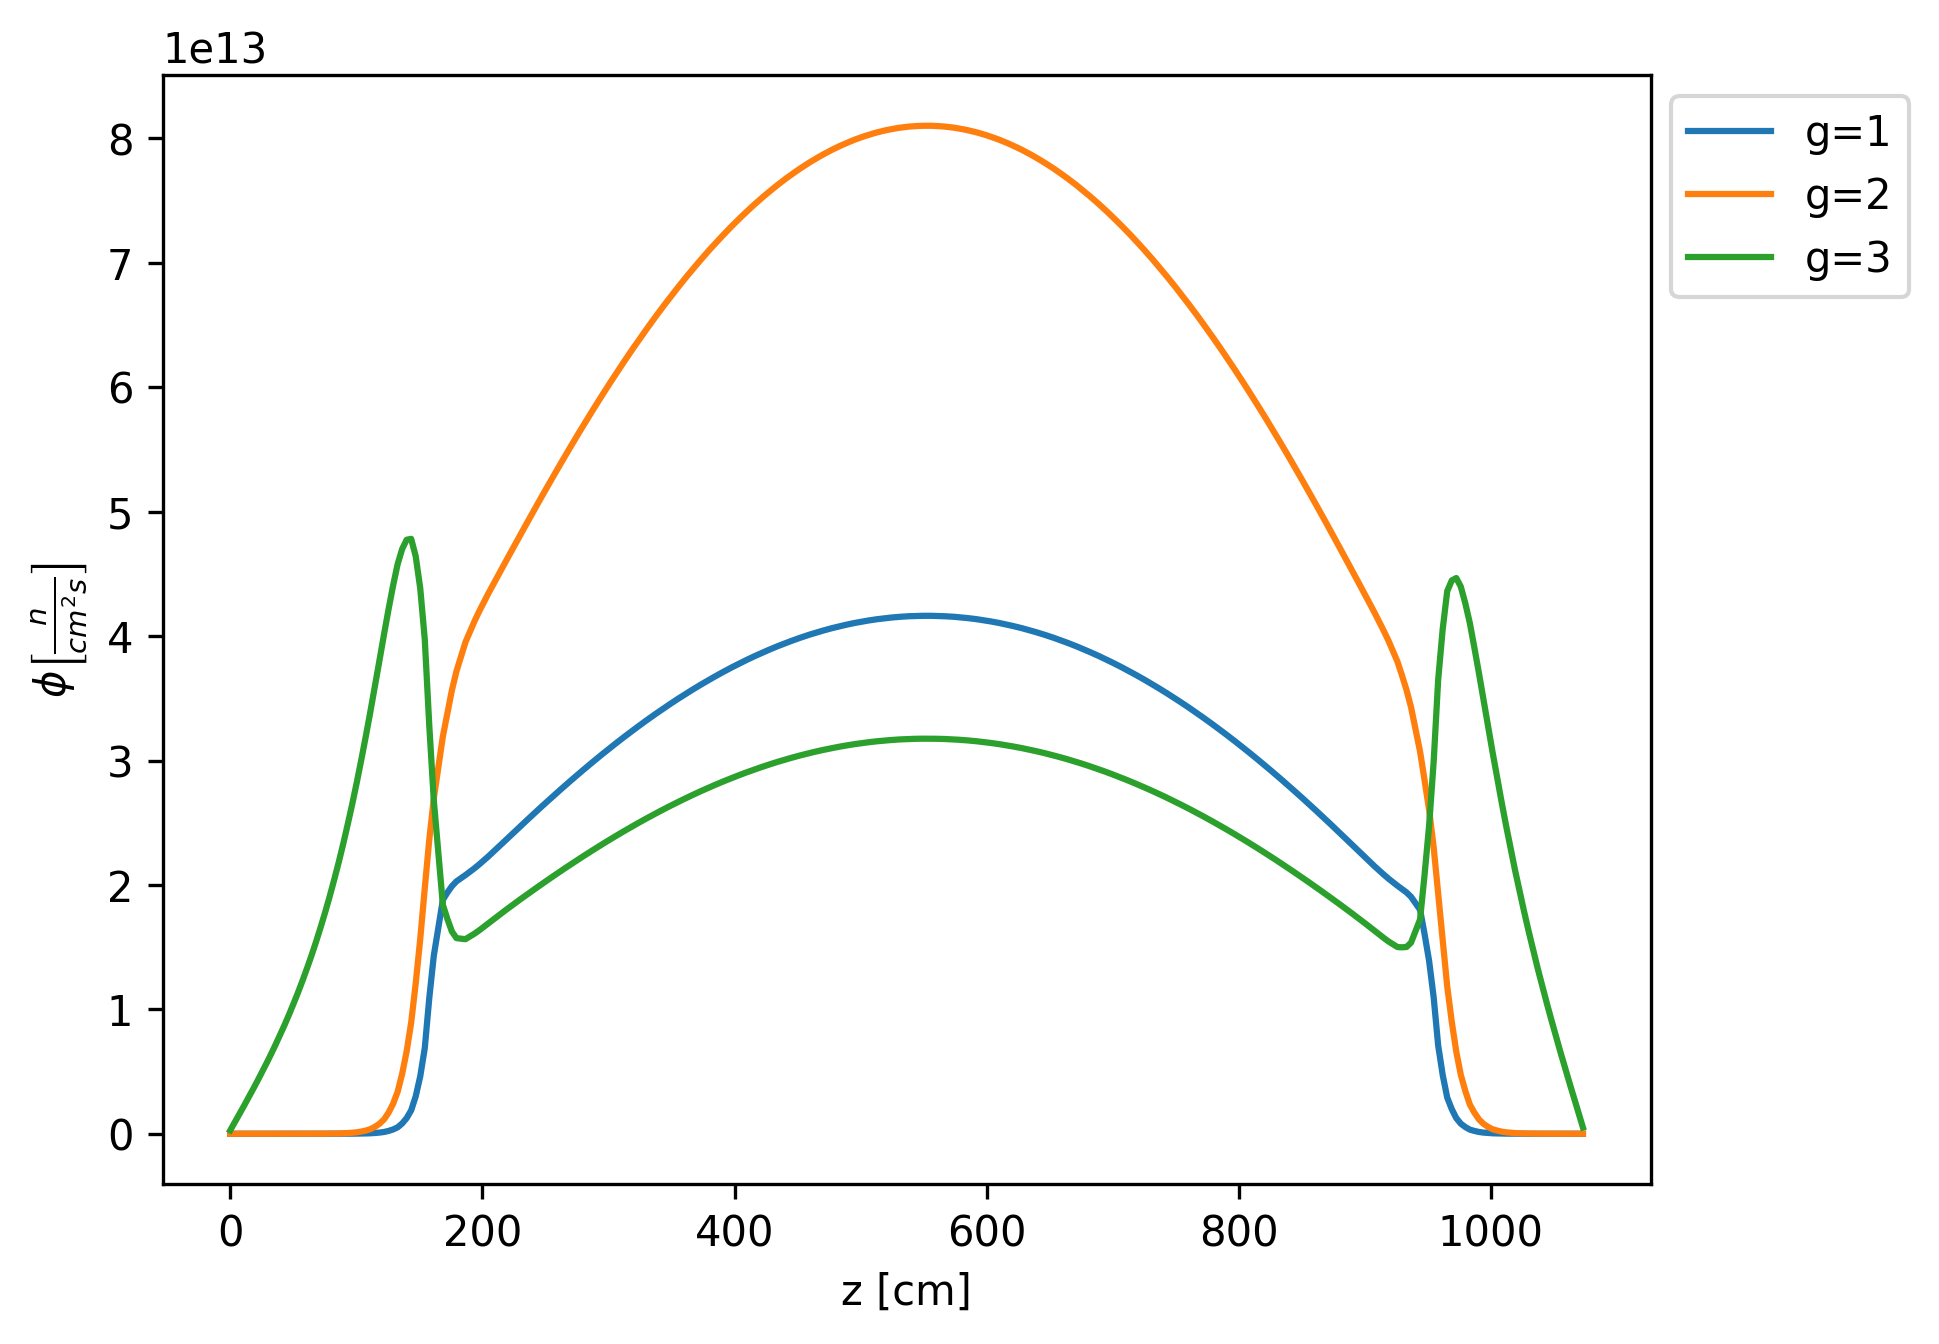
\includegraphics[width=0.45\textwidth]{figures-neutronics/3D-fullcore-1200-15Gc-axial1}
    }
	\hfill
	\caption{Comparison of the axial detector flux calculated by Serpent and Moltres at 1200 K.}
	\label{fig:fullcore-1200-axial1}
\end{figure}

%Radial flux at 1200 K
\begin{figure}[htbp!]
	\centering
    \subfloat[Serpent radial detector flux.]{
        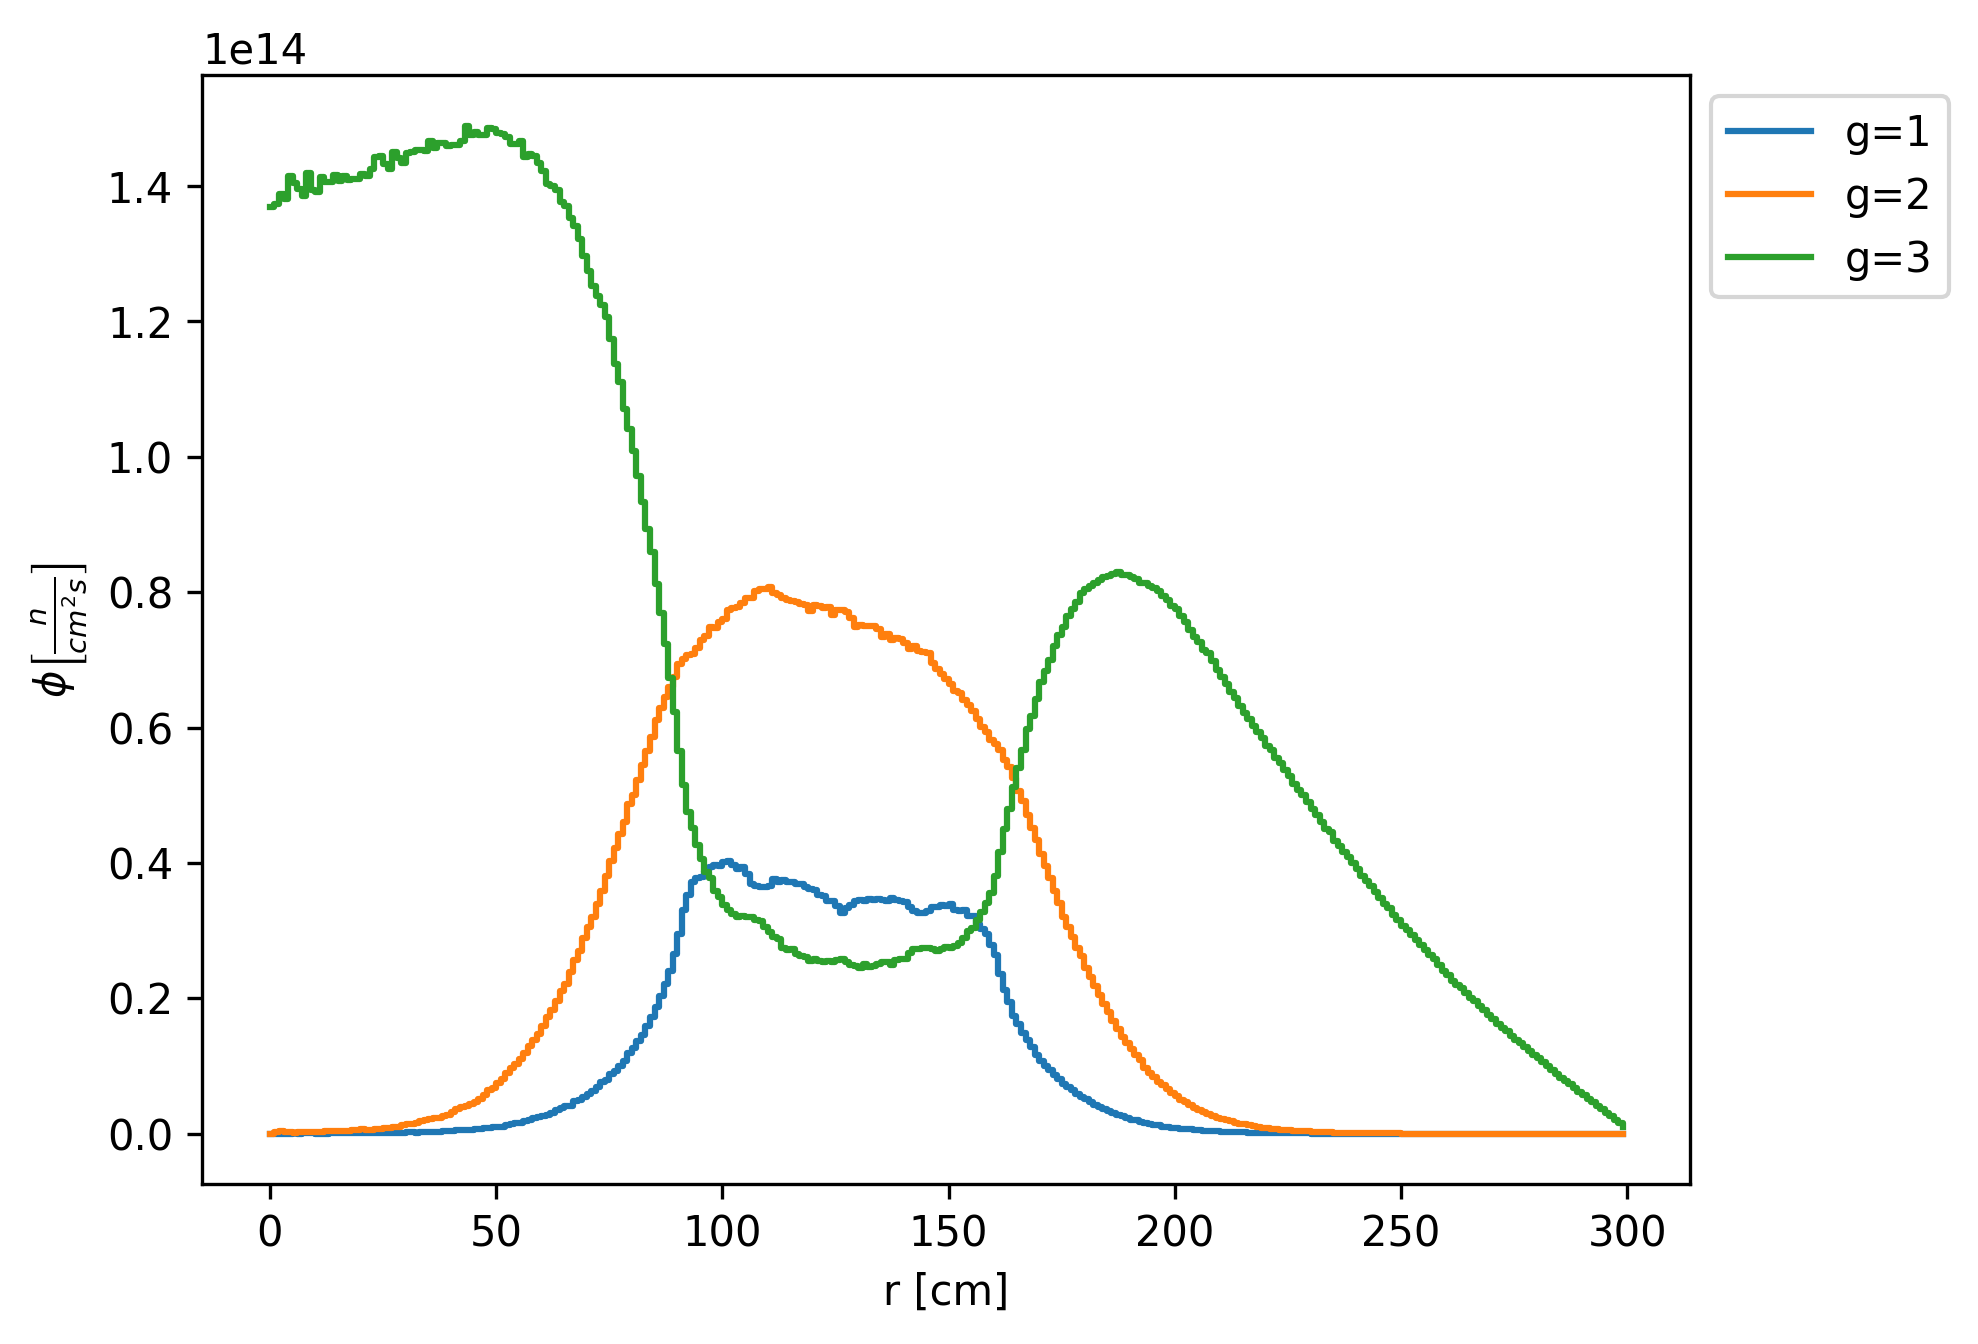
\includegraphics[width=0.45\textwidth]{figures-neutronics/serpent26G-1200-collapse-Radial}
    }
    \subfloat[Moltres radial detector flux.]{
        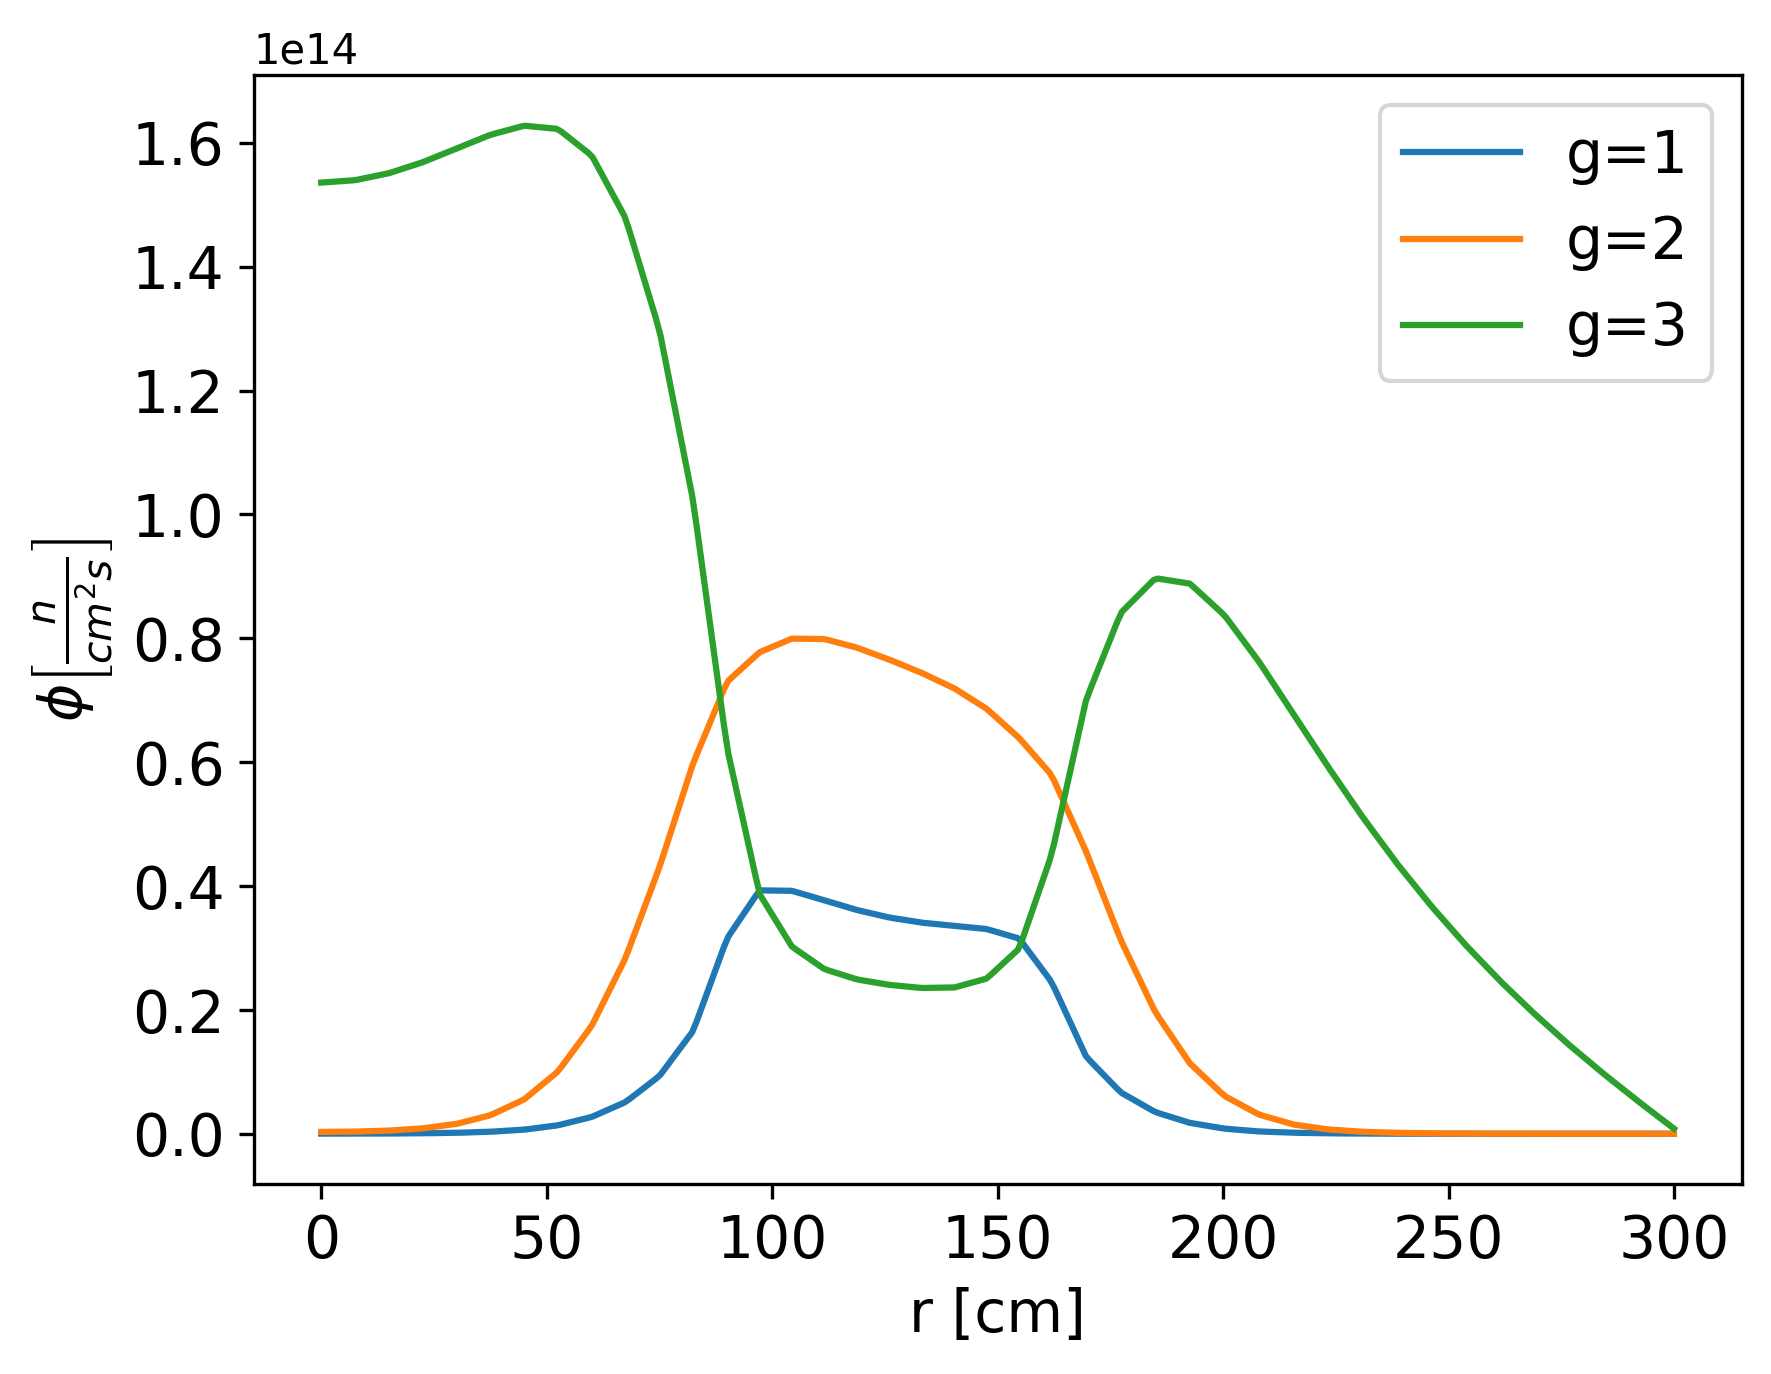
\includegraphics[width=0.45\textwidth]{figures-neutronics/3D-fullcore-1200-15Gc-radial1}
    }
	\hfill
	\caption{Comparison of the radial detector flux calculated by Serpent and Moltres at 1200 K.}
	\label{fig:fullcore-1200-radial1}
\end{figure}


\section{OECD/NEA MHTGR-350 Benchmark: Phase I Exercise 1}
\label{sec:ph1e1}

% Exercise description
This section discusses Phase I Exercise 1 of the OECD/NEA MHTGR-350 Benchmark conducted with Moltres and compares the results with those already published \cite{oecd_nea_coupled_2020}.
The benchmark specifies the group constants required to conduct the exercise, ensuring a common dataset among various benchmark participants and allowing stand-alone neutronic comparison without thermal-fluids feedback.
The exercise requests the reporting of the global parameters: $K_{eff}$, control rod worth ($\Delta \rho_{CR}$), axial offset ($AO$), and the power distribution map \cite{oecd_nea_benchmark_2017}.
Equations \ref{eq:controlrod} and \ref{eq:ao} define $\Delta \rho_{CR}$ and $AO$
\begin{align}
    \Delta \rho_{CR} &= \frac{k_{eff, out}-k_{eff, in}}{k_{eff, out}k_{eff, in}} \label{eq:controlrod}
    \intertext{where}
    \Delta \rho_{CR} &= \mbox{control rod worth} [-] \notag \\
    k_{eff, out} &= \mbox{eigenvalue with \gls{CR} out (at position z=911.7 cm)} [-] \notag \\
    k_{eff, in} &= \mbox{eigenvalue with \gls{CR} in (at position z=99 cm)} [-] \notag
		\intertext{and}
    AO &= \frac{P_{top}-P_{bottom}}{P_{top}+P_{bottom}} \label{eq:ao}
    \intertext{where}
    AO &= \mbox{axial offset } [-] \notag \\
    P_{top} &= \mbox{total power produced in the top half core } [W] \notag \\
    P_{bottom} &= \mbox{total power produced in the bottom half core } [W]. \notag
\end{align}

The Moltres simulation modeled $1/3^{rd}$ of the reactor, shown in Figure \ref{fig:bench-mesh}.
The model included the bottom and top reflectors
Two hundred and thirty-two hexagonal subdomains comprised the core, for which the benchmark provides group constants.
% Table \ref{tab:mac-region} lists the six macroscopic regions that we can differentiate in the model.
The simulations required two meshes: one for the CR out and one for the CR in.
The simulation with the CR out had 2.7 $\times 10^5$ \glspl{DoF} per energy-group, and a total of 7.0 $\times 10^6$ DoFs.
The simulation with the CR in had 2.3 $\times 10^5$ \glspl{DoF} per energy-group, and a total of 5.9 $\times 10^6$ DoFs.
The Moltres simulations obeyed an eigenvalue convergence tolerance of 1$\times$10$^{-8}$.

\begin{figure}[htbp!]
	\centering
	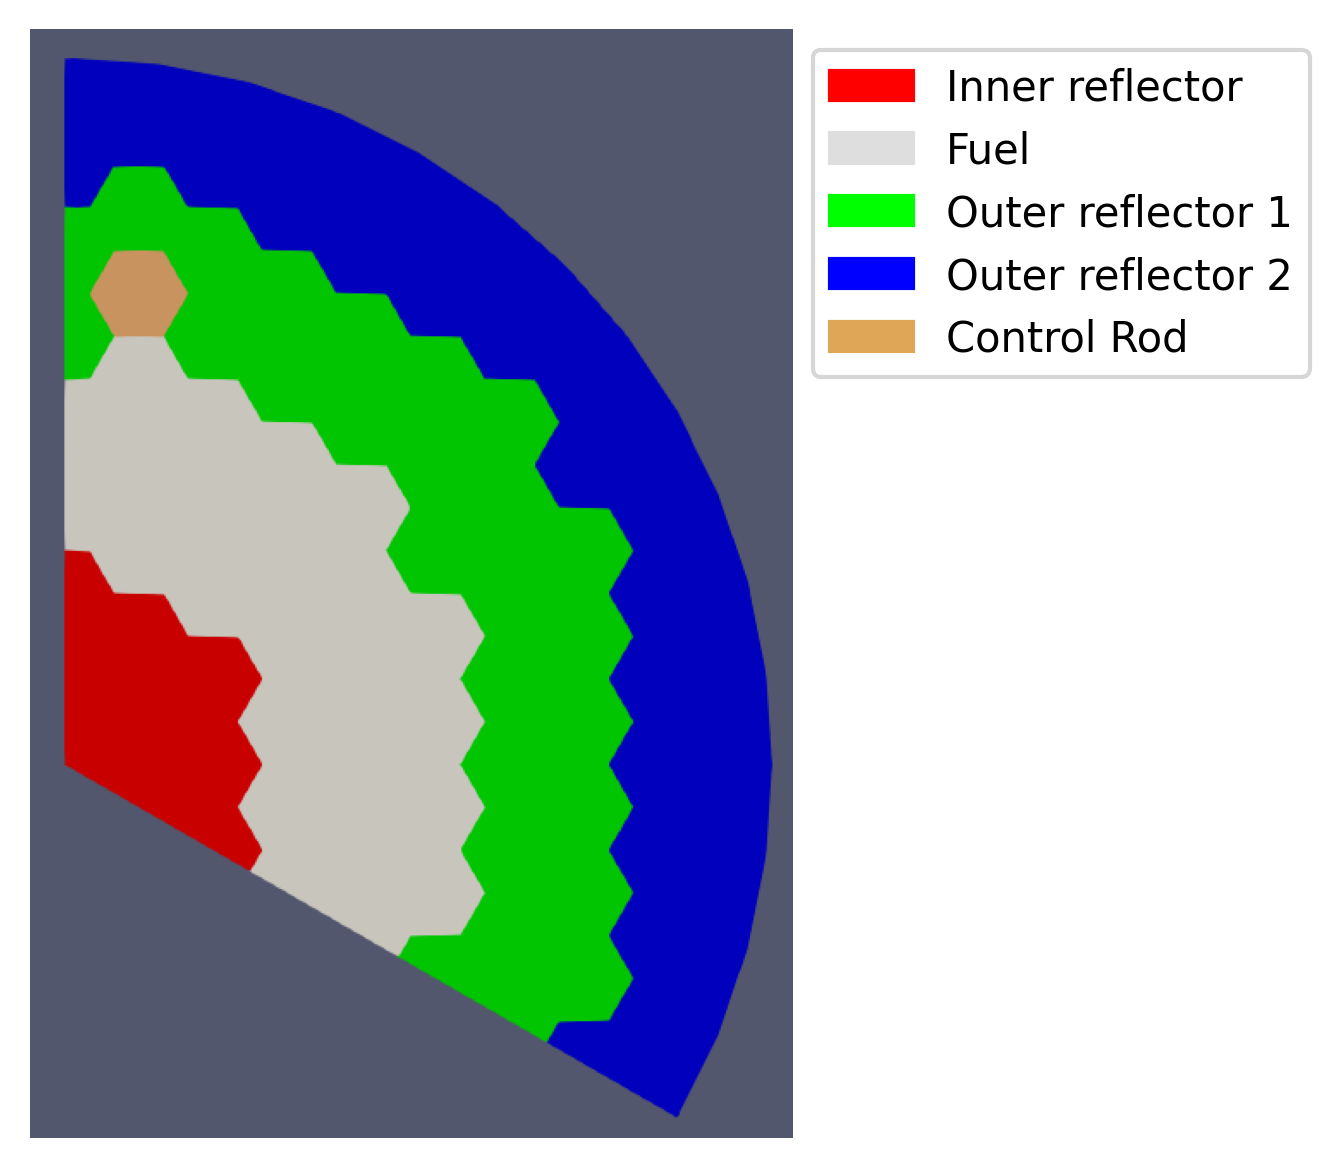
\includegraphics[width=0.55\linewidth]{figures-neutronics/oecd-fullcore-legend}
	\hfill
	\caption{Moltres model, $1/3^{rd}$ section of the MHTGR-350.}
	\label{fig:bench-mesh}
\end{figure}

% \begin{table}[htbp!]
%   \centering
%   \caption{Macroscopic regions .}
%   \label{tab:mac-region}
%   \begin{tabular}{@{}l c}
%   \toprule
%   Macroscopic region    & Subdomains     \\
%   \midrule
%   Fuel              & 1 to 220      \\
%   Bottom reflector  & 221 to 224    \\
%   Inner reflector   & 225           \\
%   Outer reflector   & 226-227       \\
%   Top reflector     & 228 to 231    \\
%   Control Rod       & 232           \\
%   \bottomrule
%   \end{tabular}
% \end{table}

The benchmark exercise specifies the group constants and a map with their location.
The benchmark definition used DRAGON-4 \cite{marleau_user_2016} to obtain the group constants from a full block configuration.
The dataset contains 26 energy groups.
Because the benchmark group constant format differs from the Moltres format, I made a Python script to handle the differences as part of this thesis.
The benchmark specifies the following group constants: $\Sigma_g^t$, $D_g$, $\nu\Sigma_g^f$, $\Sigma_g^f$, $\chi_g^t$, and $\Sigma_{g'\rightarrow g}^s$ (see equation \ref{eq:diffusion-eig}).

The benchmark exercise sets periodic \glspl{BC} on the sides of the geometry; however, a memory issue did not allow for implementing those BCs in our 26-group Moltres input file.
We approximated the periodic BC with the reflective BC.
Section \ref{sec:bench-bcs} discusses further the use of periodic and reflective BCs.

% 4.33 h and 4.11 h
On average, the simulations took 4.22 hours using 1024 cores.
Table \ref{tab:globalparam} shows the main results.
These include: Moltres predicting a \gls{Keff} larger than the reference result, a reactivity disparity of 99 pcm, Moltres yielding a smaller control rod worth (difference being 312 pcm), and the axial offset for the Moltres simulation being 4$\%$ higher than the reference result.
We attribute the discrepancies to the use of the reflective BCs instead of the periodic BCs.
Once again, Section \ref{sec:bench-bcs} discusses further the use of periodic and reflective BCs.

\begin{table}[htbp!]
  \centering
  \caption{Global parameters.}
  \begin{tabular}{lcc}
  \toprule
  Parameter 	&  Benchmark  &  Moltres    \\
  \midrule
  k$_{eff, out}$ 	&  1.06691    &  1.06804    \\
  $\Delta \rho_{CR}$ [pcm]  & 822.1 	& 509.8 \\
  AO        	&  0.168      &  0.1753     \\
  \bottomrule
  \end{tabular}
  \label{tab:globalparam}
\end{table}

Figure \ref{fig:axialpower} shows the radially averaged axial power distribution.
Figure \ref{fig:radialpower} shows the axially averaged radial power distribution.
In both figures, Moltres' values are similar to the reference results.
Moltres' power distribution in the inner ring is larger.
The differences are within 0.25 W/cm$^3$.

\begin{figure}[htbp!]
	\centering
    \subfloat[Moltres result.]{
        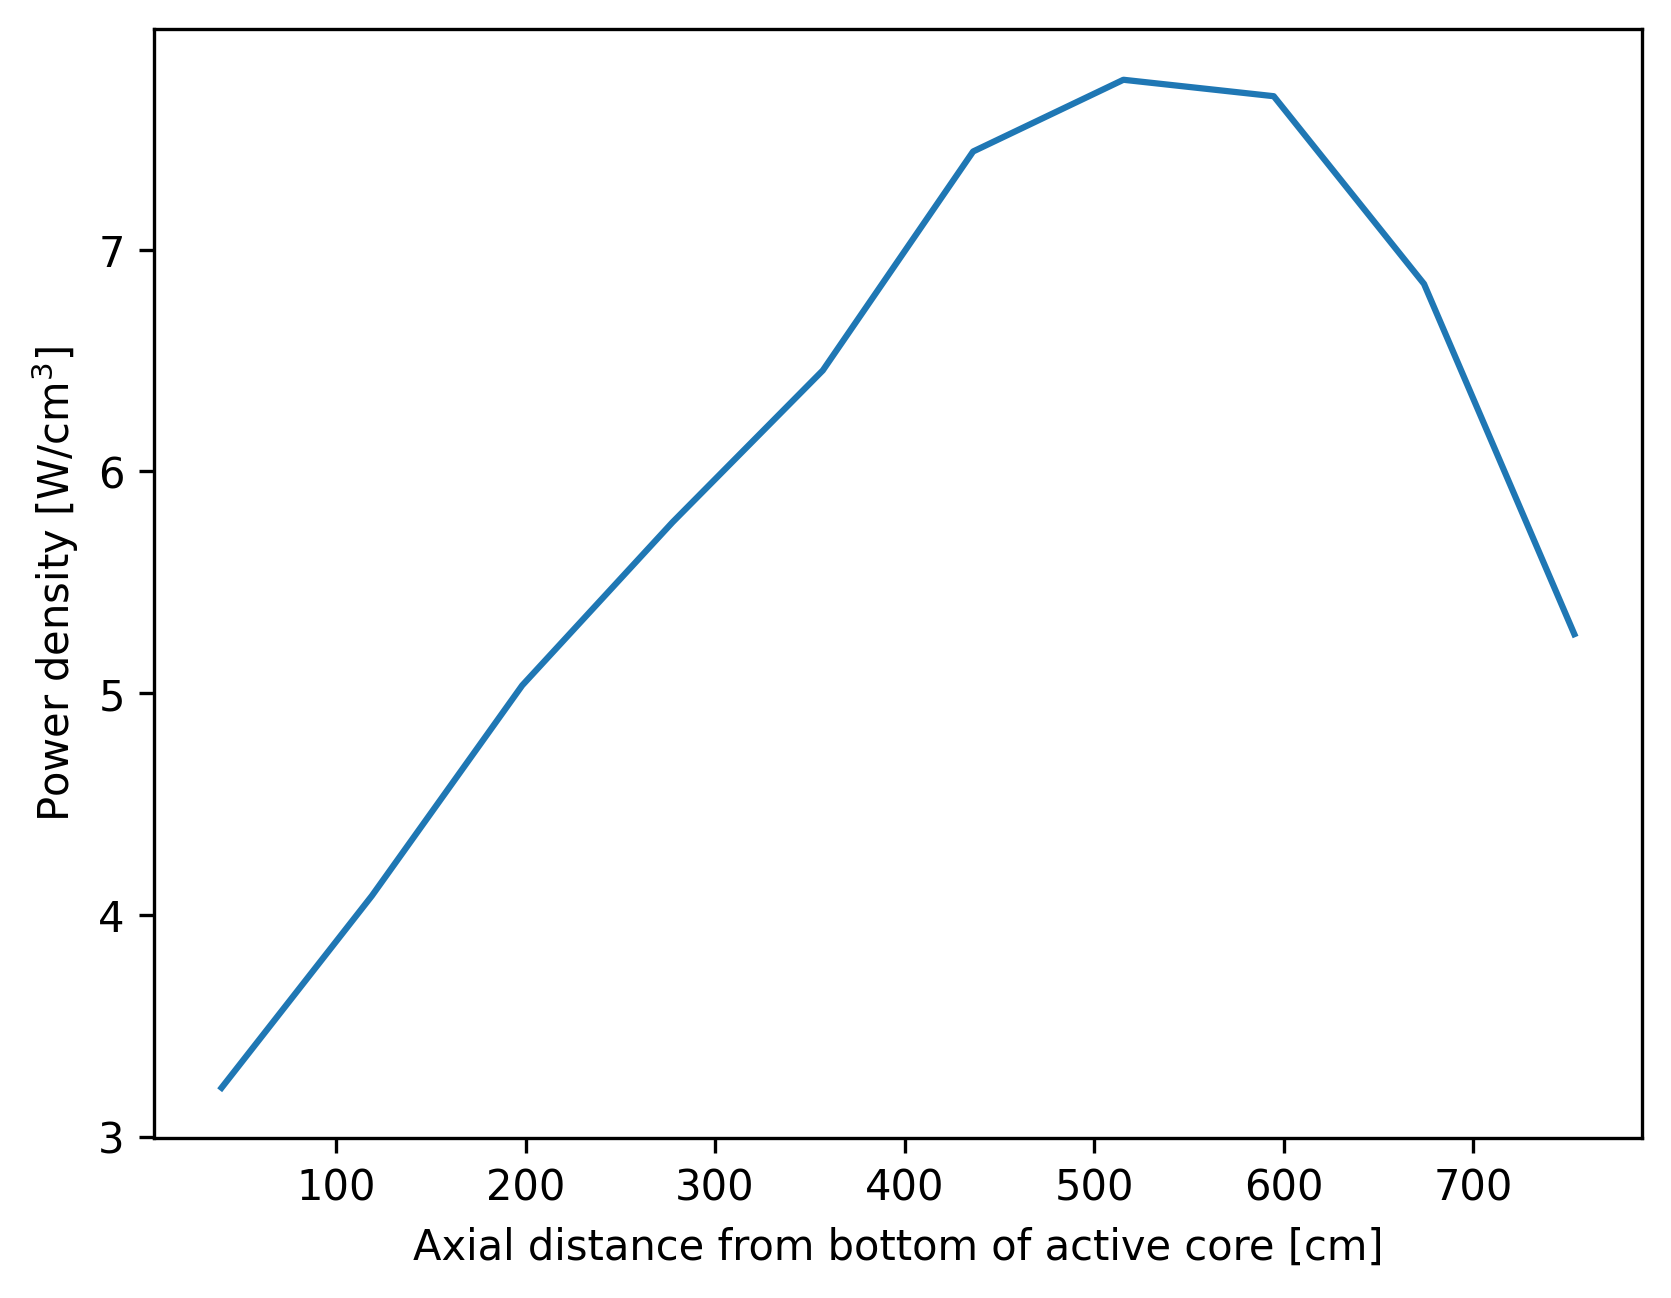
\includegraphics[width=0.42\textwidth]{figures-neutronics/3D-fullcore26G-axialpower}
    }
    \subfloat[Benchmark result. Image reproduced from \cite{oecd_nea_coupled_2020}.]{
        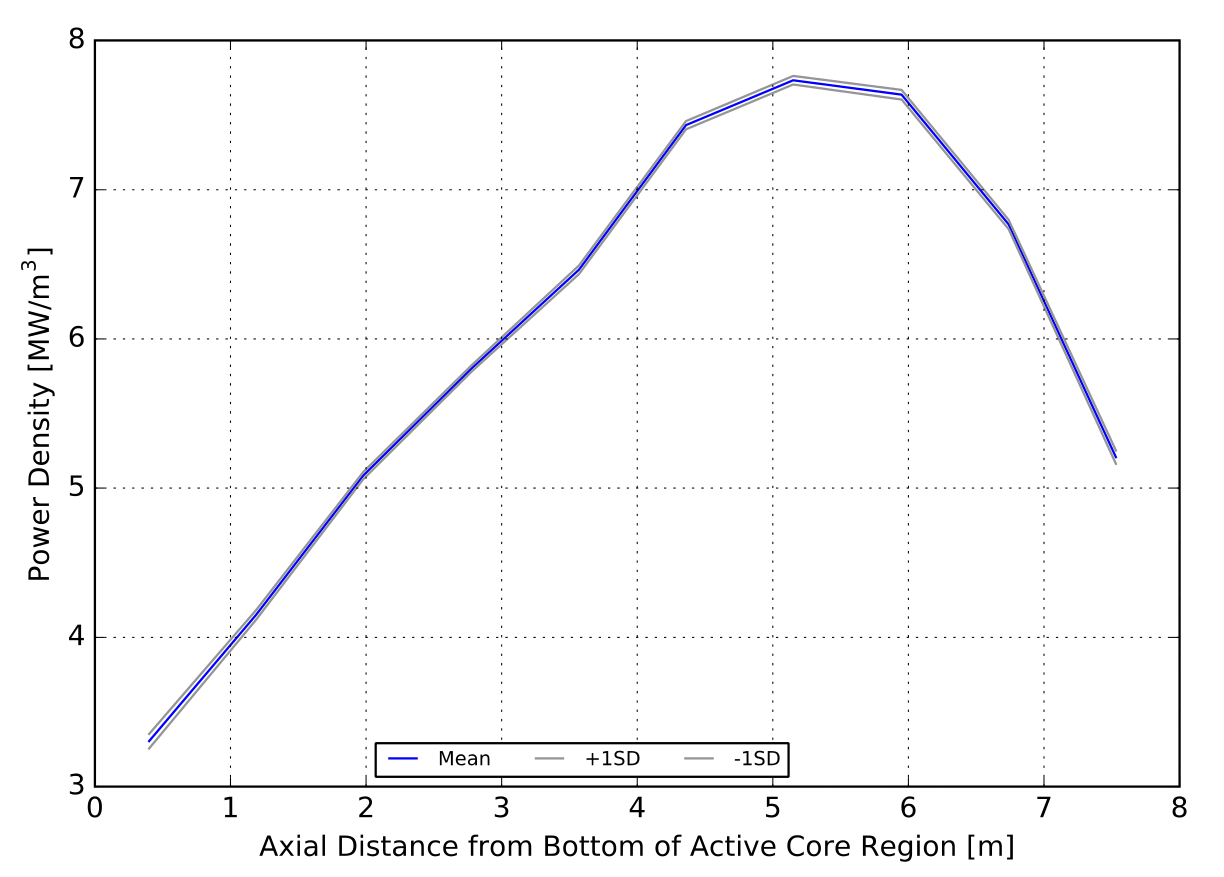
\includegraphics[width=0.47\textwidth]{figures-neutronics/benchmark-axialpower}
    }
	\hfill
	\caption{Comparison between the radially averaged axial power distribution calculated by Moltres and the benchmark published result \cite{oecd_nea_coupled_2020}.}
	\label{fig:axialpower}
\end{figure}

\begin{figure}[htbp!]
	\centering
    \subfloat[Moltres result.]{
        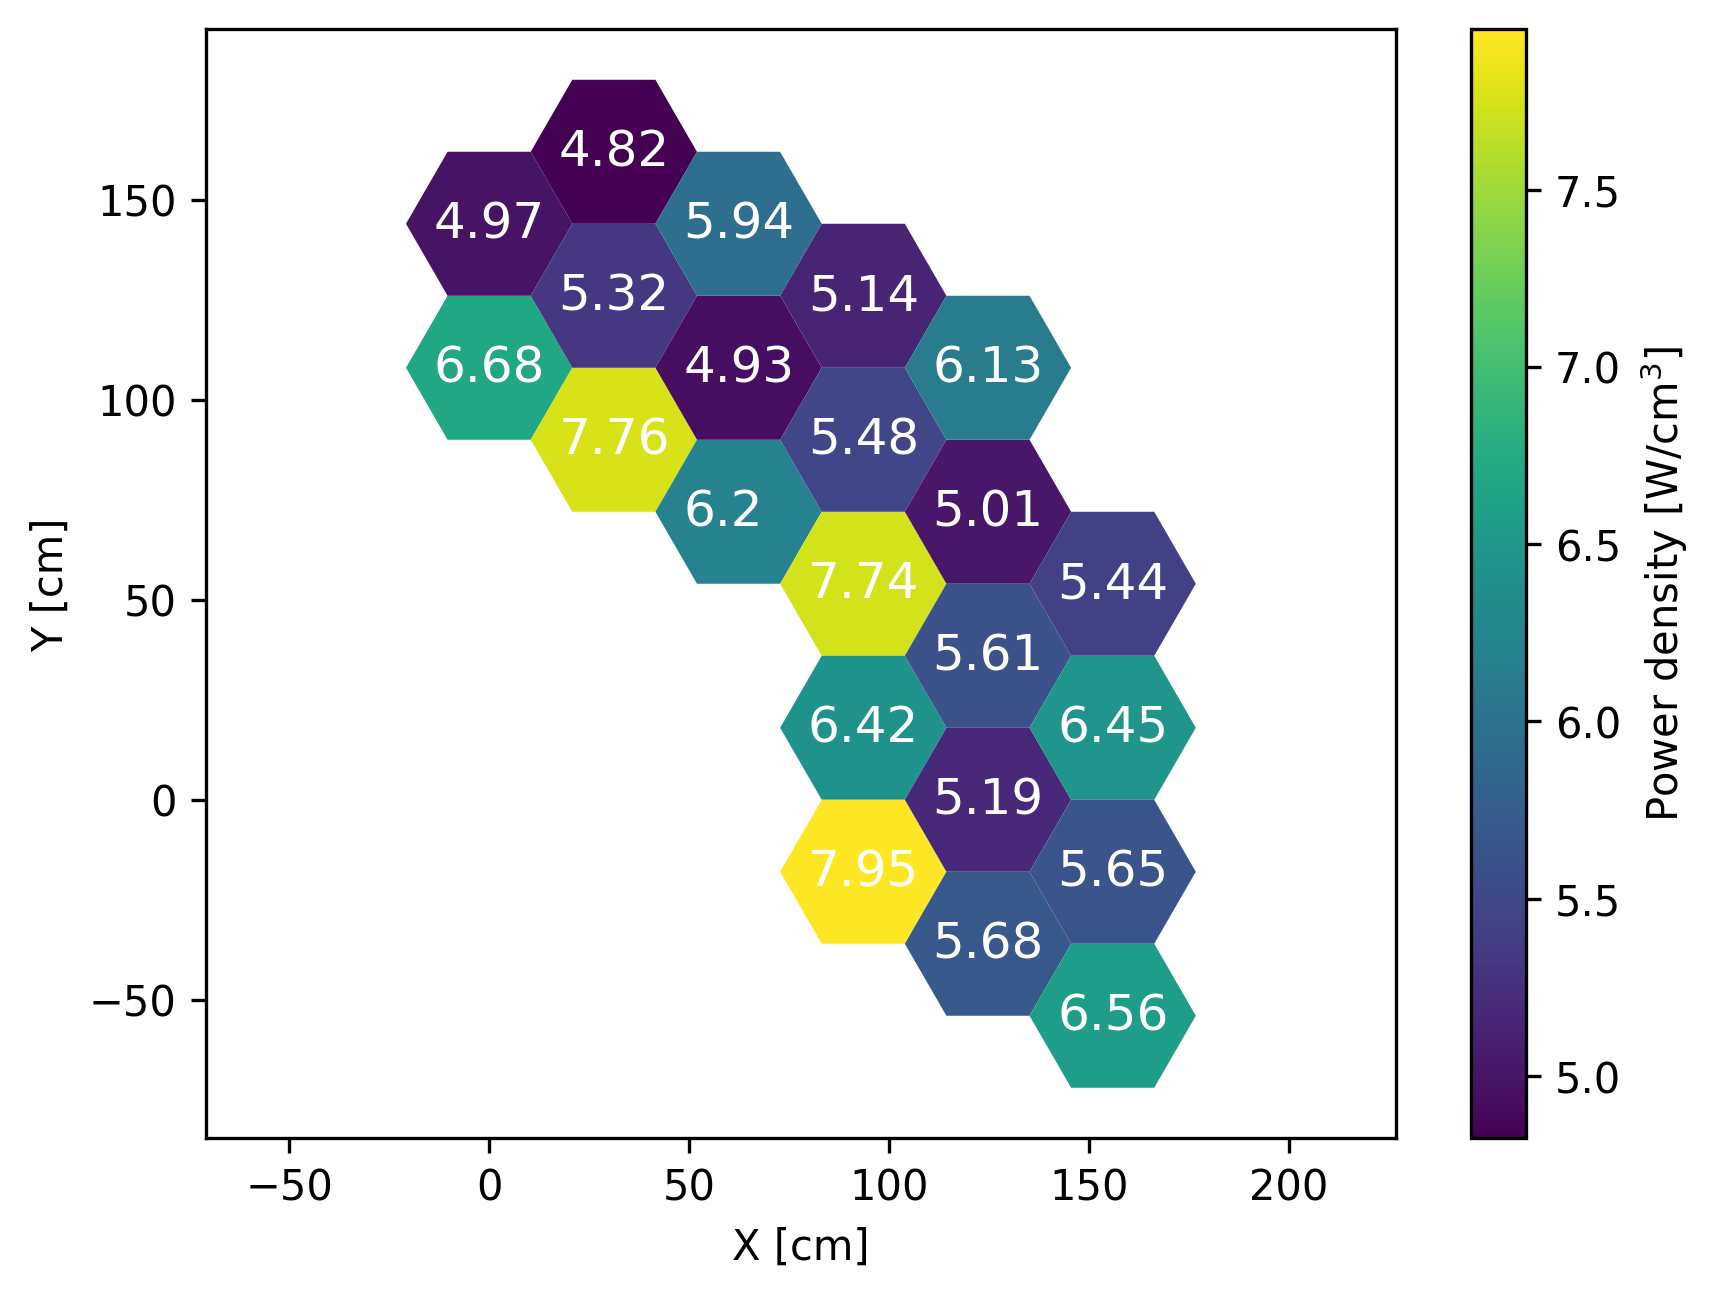
\includegraphics[width=0.47\textwidth]{figures-neutronics/3D-fullcore26G-radialpower}
    }
    \subfloat[Benchmark result. Image reproduced from \cite{oecd_nea_coupled_2020}.]{
        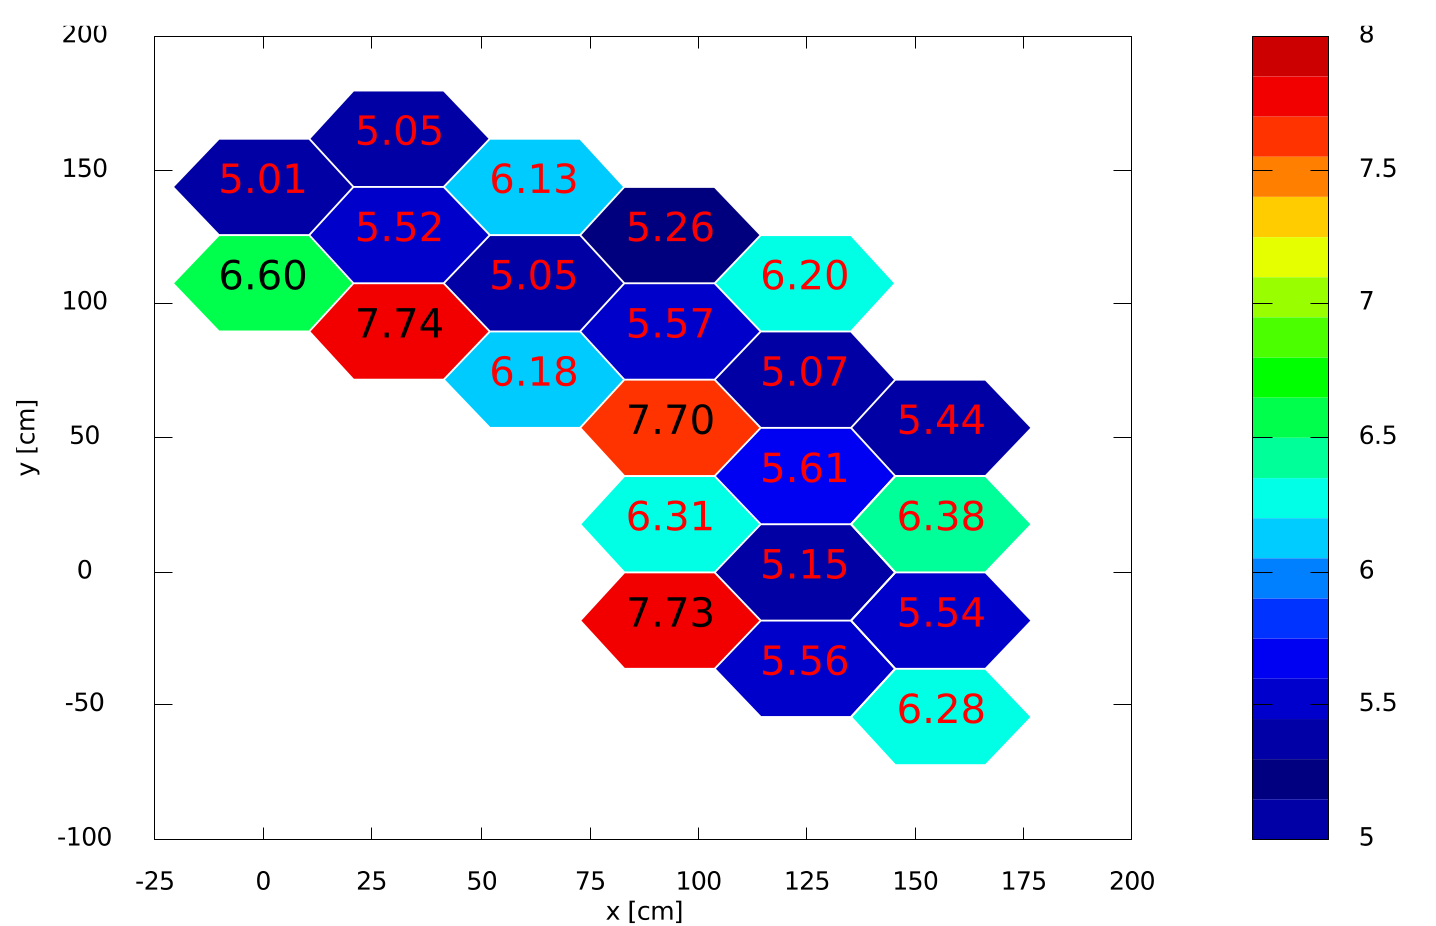
\includegraphics[width=0.42\textwidth, height=6.2cm]{figures-neutronics/benchmark-radialpower}
    }
	\hfill
  \caption{Comparison between the axially averaged radial power distribution calculated by Moltres and the benchmark published result \cite{oecd_nea_coupled_2020}.}
  \label{fig:radialpower}
\end{figure}

\subsection{Periodic vs Reflective Boundary Conditions}
\label{sec:bench-bcs}

In the last section, we observed deviations in Moltres results.
This section will analyze the discrepancies that the reflective \gls{BC} approximation may have introduced.
As the previous section mentioned, the simulation's memory requirements restrict the use of periodic BCs.
To reduce the memory requirements, we collapsed the group constants to a smaller number of energy groups.
We simulated two cases: one that uses a 3-group structure and one that uses a 6-group structure (see Table \ref{tab:energygroups}).

The simulations required two meshes each: one for the CR out and one for the CR in.
The 3-group simulation had 6.2 $\times 10^4$ DoFs per energy-group (total of 1.9 $\times 10^5$ DoFs) and 6.2 $\times 10^4$ DoFs per energy-group (total of 1.8 $\times 10^5$ DoFs) for the CR out and CR in cases, respectively.
The 6-group simulation had 1.7 $\times 10^4$ DoFs per energy-group (total of 1.0 $\times 10^5$ DoFs) and 1.9 $\times 10^4$ DoFs per energy-group (total of 1.1 $\times 10^5$ DoFs) for the CR out and CR in cases, respectively.
We highlight that the 6-group simulation had to use a coarser mesh; otherwise, it would not run.
This fact confirms the suspicion that the simulation's memory requirements prevent it from running.

We ran simulations with periodic and reflective boundary conditions for both cases and compared their results, as seen in Table \ref{tab:benchmark-bc}.
k$_{eff}$ rises with the reflective BC.
With the CR out, the raise is small.
However, with the CR in, the increase is considerable.
The combined effect of both increases leads to a decrease in the control rod worth.
The BC approximation barely affects the axial offset.

\begin{table}[htbp!]
  \centering
  \caption{Global parameter comparison for different types of BCs.}
  \begin{tabular}{clcccc}
  \toprule
  Energy groups       & Type of BCs & k$_{eff, out}$ & k$_{eff, in}$ & $\Delta \rho_{CR}$ [pcm] & AO \\
  \midrule
  \multirow{2}{*}{3}  & Periodic     & 1.07571		& 1.06776		& 692.6		& 0.237		\\
                      & Reflective   & 1.07586	  & 1.07021   & 490.5		& 0.237	  \\ \hline
  \multirow{2}{*}{6}  & Periodic     & 1.07182		& 1.06356		& 724.3	  & 0.185  	\\
                      & Reflective   & 1.07197   	& 1.06610 	& 513.3		& 0.186		\\  
  \bottomrule
  \end{tabular}
  \label{tab:benchmark-bc}
\end{table}

\section{Conclusions}
\label{sec:neutr-conc}

% Preliminary studies: homogeneous vs heterogeneous isotopic distribution
The preliminary studies focused on several aspects of the simulations.
The first aspect was the effect of distributing the fuel compact isotopes homogeneously in the Serpent model.
The results showed that the homogenization of the fuel compact isotopes decreased the multiplication factor considerably, and that the heterogeneous calculation took 28$\%$ longer.
Additionally, the homogeneous distribution appeared not to have a substantial impact on the group constants.
However, the multiplication factor's considerable difference suggested that the combined effect of the group constants’ small variations was significant.
Although explicit modeling of the TRISO particles is time-consuming, it is necessary.

% Preliminary studies: homogeneous vs heterogeneous diffusion simulation
The next section studied the problem set-up in Moltres.
Moltres uses a heterogeneous diffusion solver, making it applicable to reactor technologies that allow for heterogeneous diffusion calculations.
In this work, we aimed to use Moltres to solve prismatic HTGRs.
Nevertheless, the diffusion approximation fails to properly model regions where the mean free path is comparable to the region's dimensions.
The presence of helium in the prismatic HTGR fuel assembly challenges some of the diffusion theory assumptions.
Based on this discussion, we adapted the input group constants to carry out a homogeneous diffusion calculation using Moltres.

% Serpent-Moltres: Fuel column
Focusing on a fuel column of the MHTGR-350, we investigated the effects of the energy group structure on the diffusion calculations.
We considered four operational cases: a fuel column without burnable poisons and a fuel column with burnable poisons, both cases at 600K and 1200K.
Serpent obtained the homogenized group constants of the fuel column.
Then, Moltres took such constants as input along with a three-dimensional mesh defining the core geometry.
The first study compared the Moltres-derived axial flux to Serpent-derived axial flux.
Overall, the axial fluxes were close in shape and magnitude.
A different study focused on the effects of the energy group structure on the \gls{Keff}.
The number of energy groups did not affect the accuracy of the Moltres eigenvalue calculations.
We also compared the $L_2$-norm of the axial flux relative difference in the active core using various energy group structures.
For the four operational cases, increasing the number of energy groups improved the accuracy.
Additionally, we presented the simulation's computational expense for the different number of energy groups.
The simulation time and memory requirement rose by increasing the number of energy groups.
Finally, we analyzed the impact of using different 15-group structures on the $L_2$-norm of the axial flux relative error.
We chose $15d$ as the best-performing energy group structure.

% Serpent-Moltres: Full-core
Based on the fuel column analysis results, we compared Moltres full-core results with Serpent reference results.
We considered two operational cases: 600K and 1200K.
Serpent obtained the homogenized group constants of the different regions of the reactor, and again, Moltres took such constants as input along with a three-dimensional mesh.
The first analysis compared the Serpent and Moltres eigenvalues --- Moltres results were bigger, but the overall differences were less than 300 pcm.
The second analysis compared the radial power distributions from both codes.
These results showcased the symmetry of the problem.
Reducing the problem size by half, other simulations could reduce their computational expense.
For the most part, Moltres radial power distribution showed proximity to the Serpent's result.
We also compared Moltres and Serpent fluxes in two directions (axial and radial) in arbitrary core regions.
The axial fluxes showed small discrepancies, mostly in their magnitude.
The radial fluxes were close in shape and magnitude; however, the radial flux in the diffusion calculation failed to capture the flux variation near the burnable poisons.
Overall, the fluxes were similar.

% OECD-Benchmark
The simulation capabilities for prismatic HTGRs have not reached state of the art of LWRs.
This development delay motivated OECD/NEA to define a benchmark, which uses the MHTGR-350 as the reference design, to carry out code-to-code comparisons.
We conducted Phase I Exercise 1 with Moltres, using the group constants defined by the benchmark.
The group constants have a 26-energy group structure, and the exercise sets periodic \glspl{BC} on the sides of the geometry.
The simulation's high memory requirements have challenged such implementation in Moltres.
To circumvent this, we approximated the periodic \gls{BC} with a reflective BC.
Two out of three global parameters exhibited good agreement with the reference results; however, the control rod worth presented a large discrepancy, a consequence of the BC approximation.
Reducing the problem's size by collapsing the group constants to 3 and 6-energy groups, we compared the \gls{Keff} using the periodic and reflective BCs.
A reflective BC for the \gls{CR} out case did not substantially impact the \gls{Keff}, but the BC choice for the CR in case had a significant effect.
The combined effect of the approximation led to a large error in the CR worth, while it had only a small influence on the axial offset.

\chapter{Thermal-Hydraulics}
MMR
Outlet Temperature: 630$^{\circ}$C
Power Density: 1.24 $W/cm^3$
\cite{usnc_mmr_2019}


Analysis with three axial power profiles.
A- Continuous cosine profile.
B- Discontinuous and uniform.
C- Axial power profile at EOC of the equilibrium core.
Sharp drops due to non fuel zones at the interfaces between the fuel blocks (graphite plugs and seats). Plugs and seats of 2 cm thickness located at the top and bottom positions of the fuel blocks.
\cite{tak_practical_2012}

\chapter*{Appendix}
\section{Verification of the thermal-fluids model}
\label{appendix:ver}

The analytical solution of this problem is
\begin{align}
    T_c (r, z) &= T_{in} + \frac{q_{ave} R_f^2 L}{2 \rho c_p v \pi R_c^2} \left[ 1 + cos \left( \frac{\pi}{L} z \right) \right] \\
    T_3(z) &= T_c(z) + \frac{q_{ave} \pi}{2} sin \left( \frac{\pi}{L} z \right) R_f^2 \frac{ln(R_i/R_m)}{2 k_i} \\
    T_2(z) &= T_3(z) + \frac{q_{ave} \pi}{2} sin \left( \frac{\pi}{L} z \right) R_f^2 \frac{ln(R_m/R_g)}{2 k_m} \\
    T_1(z) &= T_2(z) + \frac{q_{ave} \pi}{2} sin \left( \frac{\pi}{L} z \right) R_f^2 \frac{ln(R_g/R_f)}{2 k_g} \\
    T_f (r=0, z) &= T_1(z) + \frac{q_{ave} \pi}{2} sin \left( \frac{\pi}{L} z \right) R_f^2 \frac{1}{4 k_f} \\
    T_f (r, z=L/2) &= \frac{q_{ave}}{4 k_f} \left(R_f^2 - r^2\right) + T_1 (z=L/2) \\
    T_g (r, z=L/2) &= \frac{T_1 (z=L/2)-T_2 (z=L/2)}{ln (R_f/R_g)} ln (r/R_g) + T_1(z=L/2) \\
    T_m (r, z=L/2) &= \frac{T_2 (z=L/2)-T_3 (z=L/2)}{ln (R_g/R_m)} ln (r/R_m) + T_2(z=L/2) \\
    T_i (r, z=L/2) &= \frac{T_3 (z=L/2)-T_c (z=L/2)}{ln (R_m/R_i)} ln (r/R_i) + T_3(z=L/2) \\
    T_c (r, z=L/2) &= T_c(z=L/2)
    \intertext{where}
    T_{c} &= \mbox{bulk coolant temperature} \notag \\
    T_{in} &= \mbox{inlet coolant temperature} \notag \\
    q_{ave} &= \mbox{average power density} \notag \\
    R_f &= \mbox{fuel compact radius} \notag \\
    L &= \mbox{fuel column height} \notag \\
    \rho &= \mbox{helium density} \notag \\
    c_p &= \mbox{helium heat capacity} \notag \\
    v &= \mbox{average helium velocity} \notag \\
    R_c &= \mbox{coolant channel radius} \notag \\
    R_g &= \mbox{gap radius} \notag \\
    R_m &= \mbox{moderator radius} \notag \\
    R_i &= \mbox{film radius} \notag \\
    k_f &= \mbox{fuel compact thermal conductivity} \notag \\
    k_g &= \mbox{gap thermal conductivity} \notag \\
    k_m &= \mbox{moderator thermal conductivity} \notag \\
    k_i &= \mbox{film thermal conductivity} = h R_i ln(R_i/R_m) \notag
\end{align}


\backmatter

\bibliographystyle{apalike}
\bibliography{bibliography}

\end{document}
\endinput
%%
%% End of file
